\chapter{Experimental Results and Discussion}
\label{sec:results}

\todo[inline]{Update plots.}
\todo[inline]{More results.}

We evaluated the in chapter \ref{chapter:alphalinkage} proposed algorithms with the in chapter \ref{chapter:datasets} discussed datasets aiming to find new subcategories for the text data and to generate better clusterings overall. The quality of the clusterings was calculated with the in chapter \ref{chapter:costfunctions} explained cost functions.

\section{Algorithm Selection}

In general we evaluate two different types of experiments that apply for most of the datasets. Only for the synthetic dataset, we evaluate the data distribution shown in figure \ref{fig:disksrings}.

\paragraph{Batch Data Experiments.} In the first one, we evaluate certain data batches, i.e. we subsample the $n$-th set of points in sorted order for each of the target classes. To generalize the experiments for larger datasets, we average over multiple batches. In our experiments, we evaluate all distinct combinations of $k$ classes, e.g. for multiple datasets we have 10 target classes and use 5 labels for our experiments, i.e. we evaluate all $10 \choose 5$ combinations to cover all possible label subsets.

\paragraph{Randomized Experiments.} In the other setting, we select the points for certain classes by random. Averaging over a large number of clustering instances allows us to cover a major fraction of the dataset. To clusters a subset of the target classes, we also select the classes by random. Overall, in case both experimental settings agree, we know that the results are generalized well for the underlying data distribution.

\paragraph{Synthetic Experiments.} Here we generated 1,000 clustering instances by random given the data distribution shown in section \ref{chapter:datasets}, i.e. all instances contain four classes, two rings and two disks. In figure \ref{fig:syntheticexperiments} we observe that all three linkage strategies perform very similarly. Only single linkage does slightly better with an error below $25\%$ while both average and complete linkage are above $25\%$. Interpolating between single and linkage (a) leads to significantly lower errors ($4.2\%$), where interpolating between average and complete linkage (b) does not lead to improvements. As this example motivates interpolating between single and complete linkage, we elaborate this setting further. Figure \ref{fig:syntheticexperiments} (c) shows that single linkage does very well identifying the two rings, while it tends to combine the two disk-shaped clusters in a quite early step. On the other hand, complete linkage does very well clustering the two disks, but it tends to combine the two rings (see figure \ref{fig:syntheticexperiments} (d)).

\begin{figure}[h]
\centering
\begin{minipage}{.45\textwidth}
  \centering
  \subcaptionbox{Interpolating between single and complete linkage justifies our motivation for the synthetic experiments as it reduces the error from $23.65\%$ to $4.21\%$.}
  {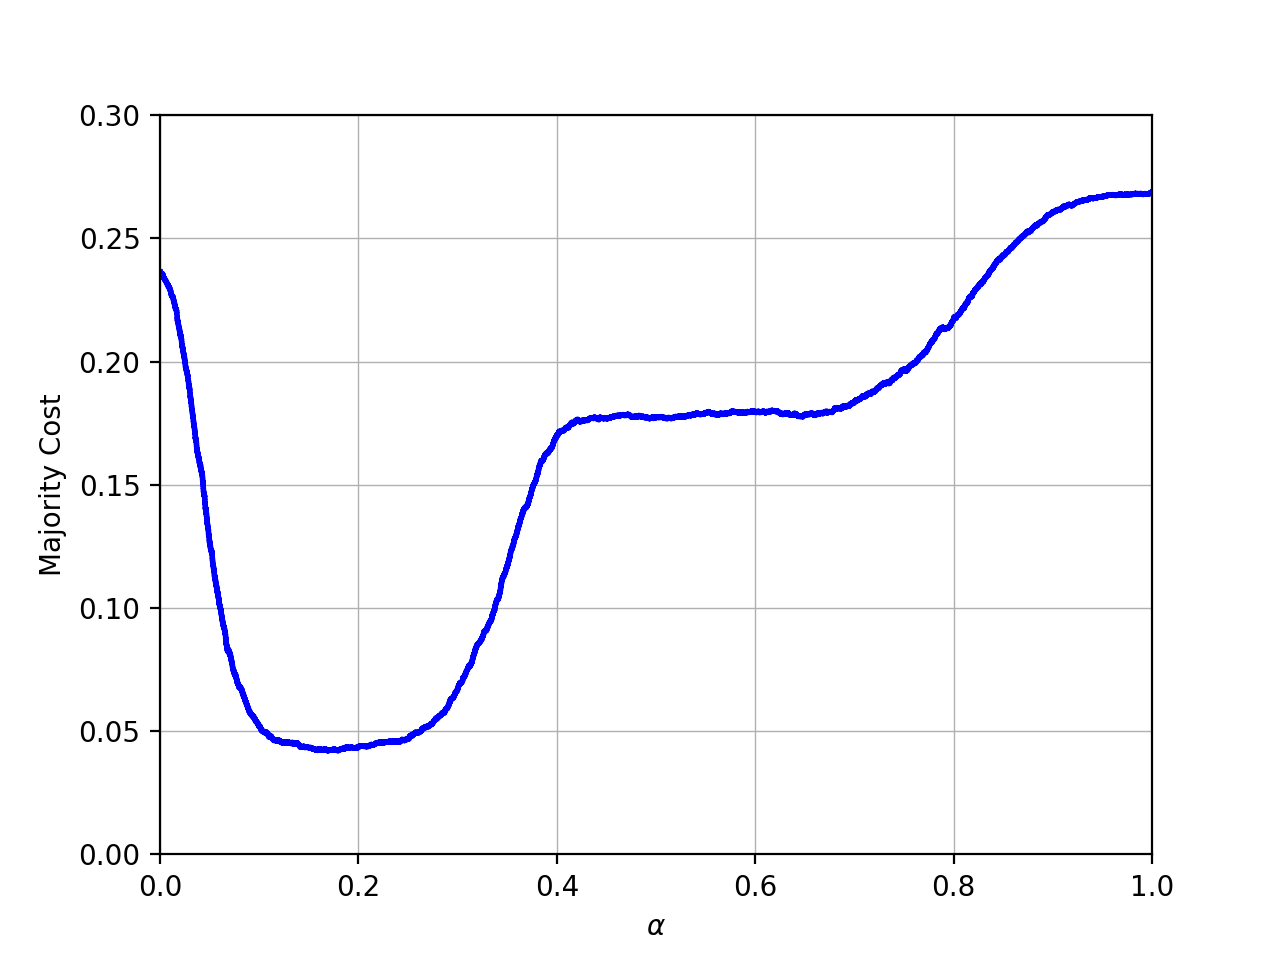
\includegraphics[width=\linewidth]{plots/ringsanddiskssc}}
\end{minipage}\qquad
\begin{minipage}{.45\textwidth}
  \centering
  \subcaptionbox{In comparison, interpolating between average and complete linkage does not lead to improvements. The error stays mostly constant around $26\%$.}
  {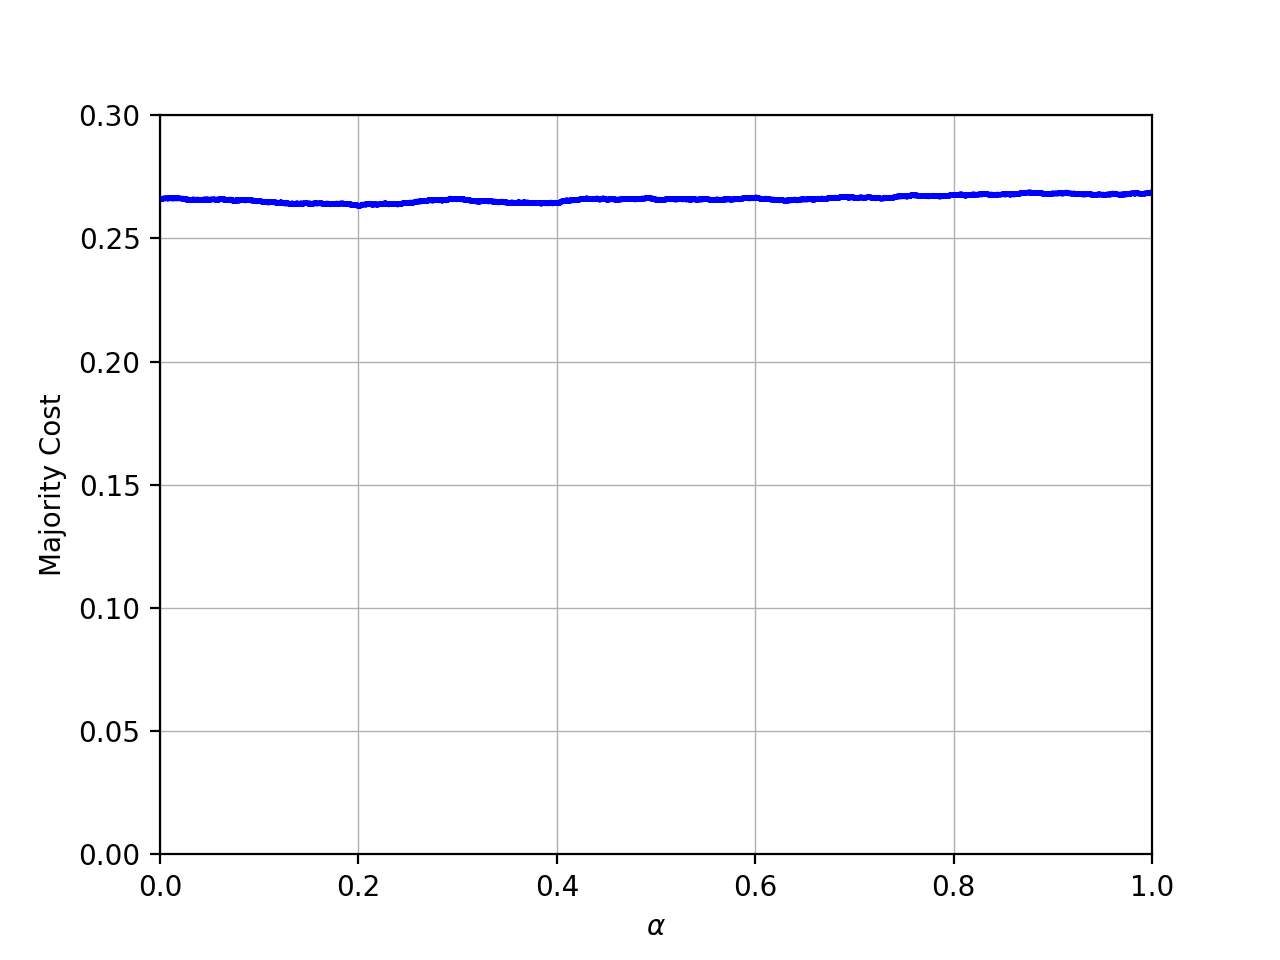
\includegraphics[width=\linewidth]{plots/ringsanddisksac}}
\end{minipage}
\begin{minipage}{.45\textwidth}
  \centering
  \subcaptionbox{Single linkage does well for the rings, however it cannot recognize the clusters in the two disks.}
  {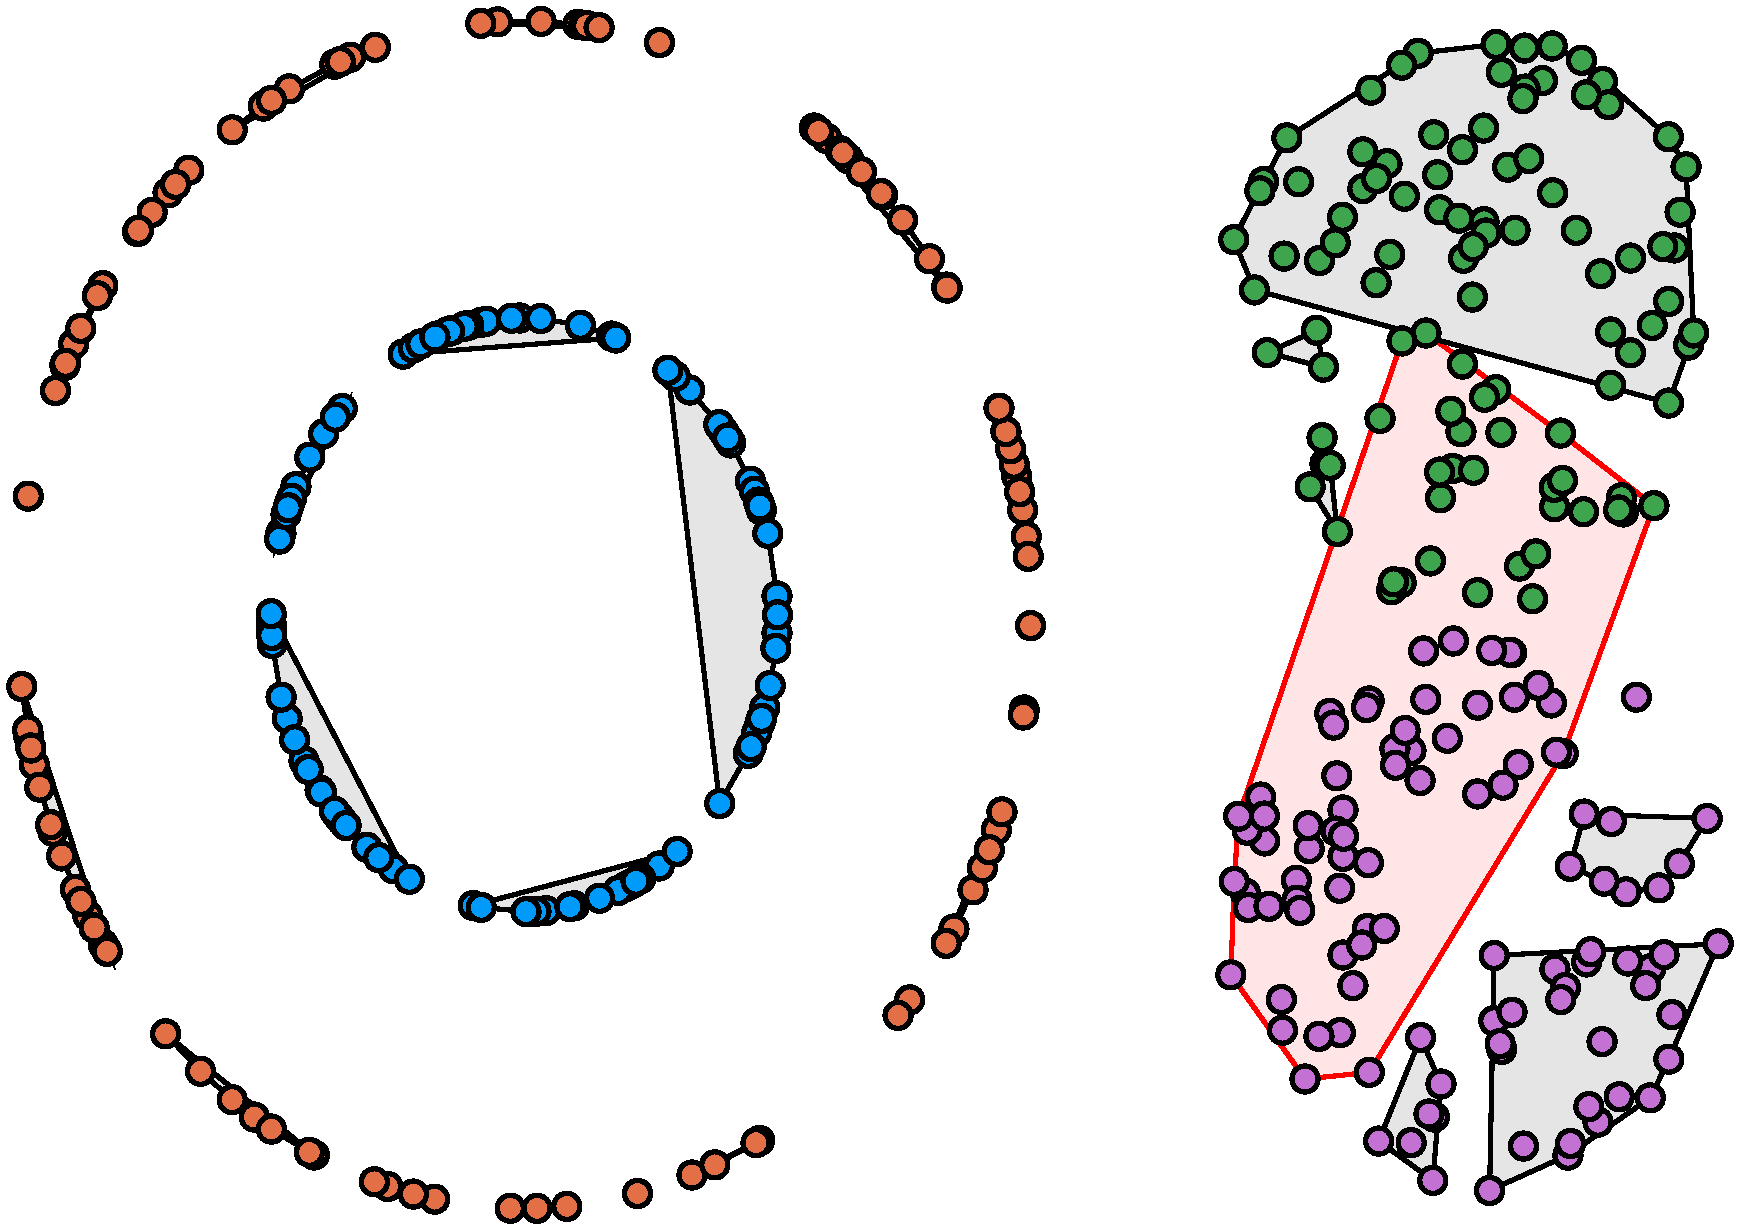
\includegraphics[width=\linewidth]{plots/single_linkage_370}}
\end{minipage}\qquad
\begin{minipage}{.45\textwidth}
  \centering
  \subcaptionbox{Complete linkage does well recognizing the disks, but it fails to correctly identify the rings.}
  {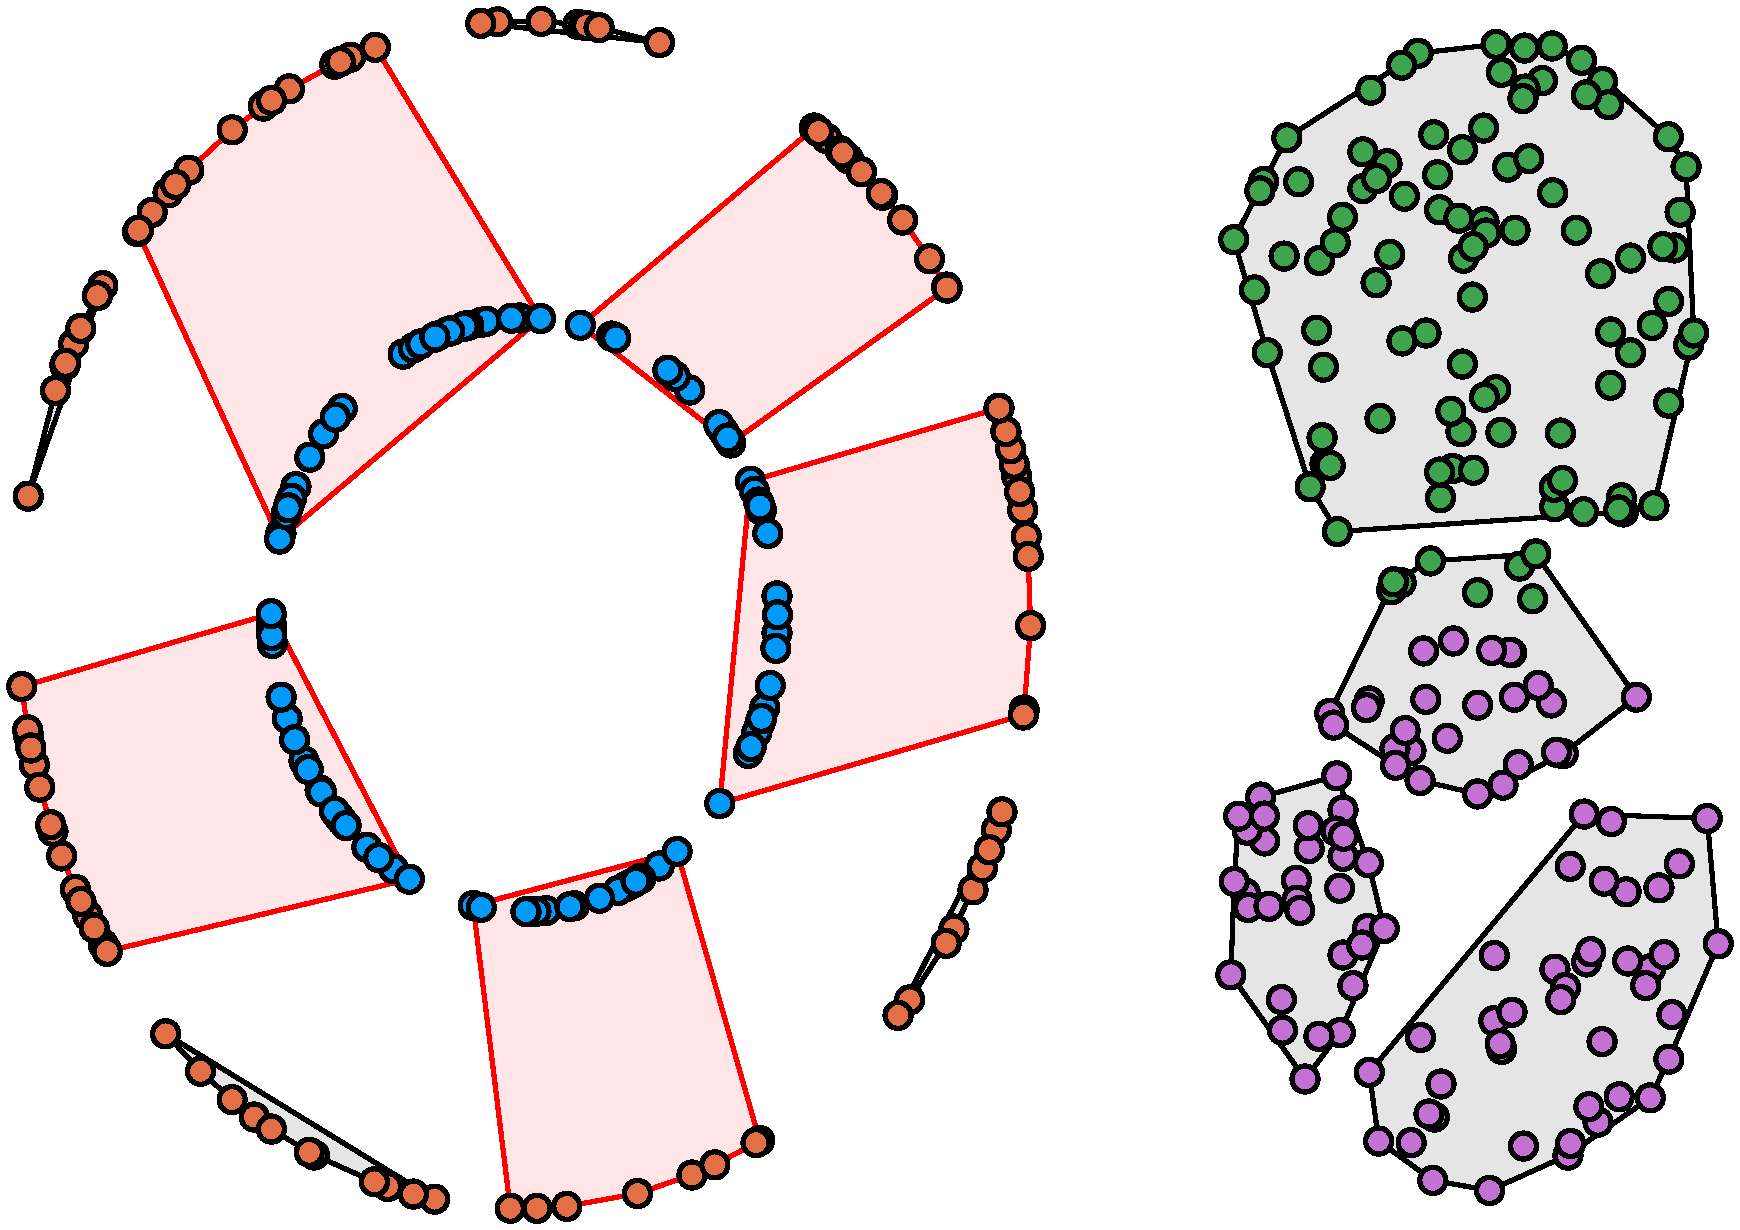
\includegraphics[width=\linewidth]{plots/complete_linkage_389}}
\end{minipage}
\caption{%
  %
  Clustering the synthetic data leads to great improvements when interpolating between single and complete linkage. We observe that single linkage is able to identify the rings very well while complete linkage recognizes the disks. A weighted combination of both is able to plot the overall data very well, while average linkage and complete linkage perform almost identically.
  }
  %
\label{fig:syntheticexperiments}
\end{figure}

\paragraph{NELL Experiments.} In order to find new subclusters for the NELL data, we cluster each of the 32 main categories seperately. This results in 32 different clustering tasks, where we compare the results of each clustering task with the target labels using the majority distance function. We will receive a cost function $cost(\alpha)$, that shows us for which value of $\alpha$ the resulting clusterings are good, for each category. By averaging all cost functions, we know for which values of $\alpha$ the $\alpha$-linkage performs well in general. Beside having a value of $\alpha$ that can be used for other clustering tasks, the experiments also give different representation levels of clusters that are discussed in section. First, we started evaluating all tasks with a maximum of 250 points per task. Figure \ref{fig:nellresults} shows the result for all three different interpolation strategies.

\begin{figure}[h]
\centering
\begin{minipage}{.3\textwidth}
  \centering
  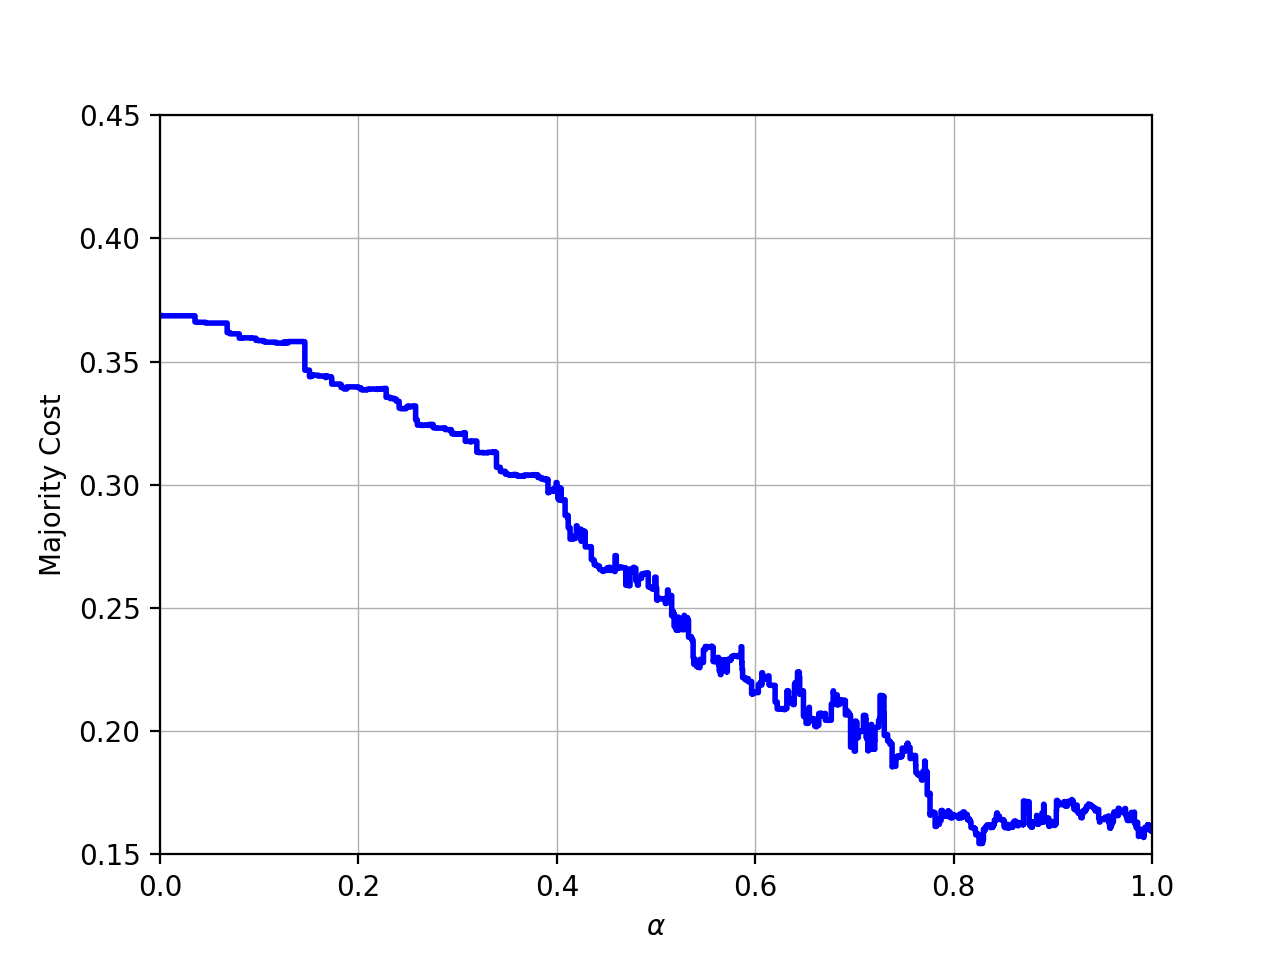
\includegraphics[width=\linewidth]{plots/nell_sc}
\end{minipage}
\begin{minipage}{.3\textwidth}
  \centering
  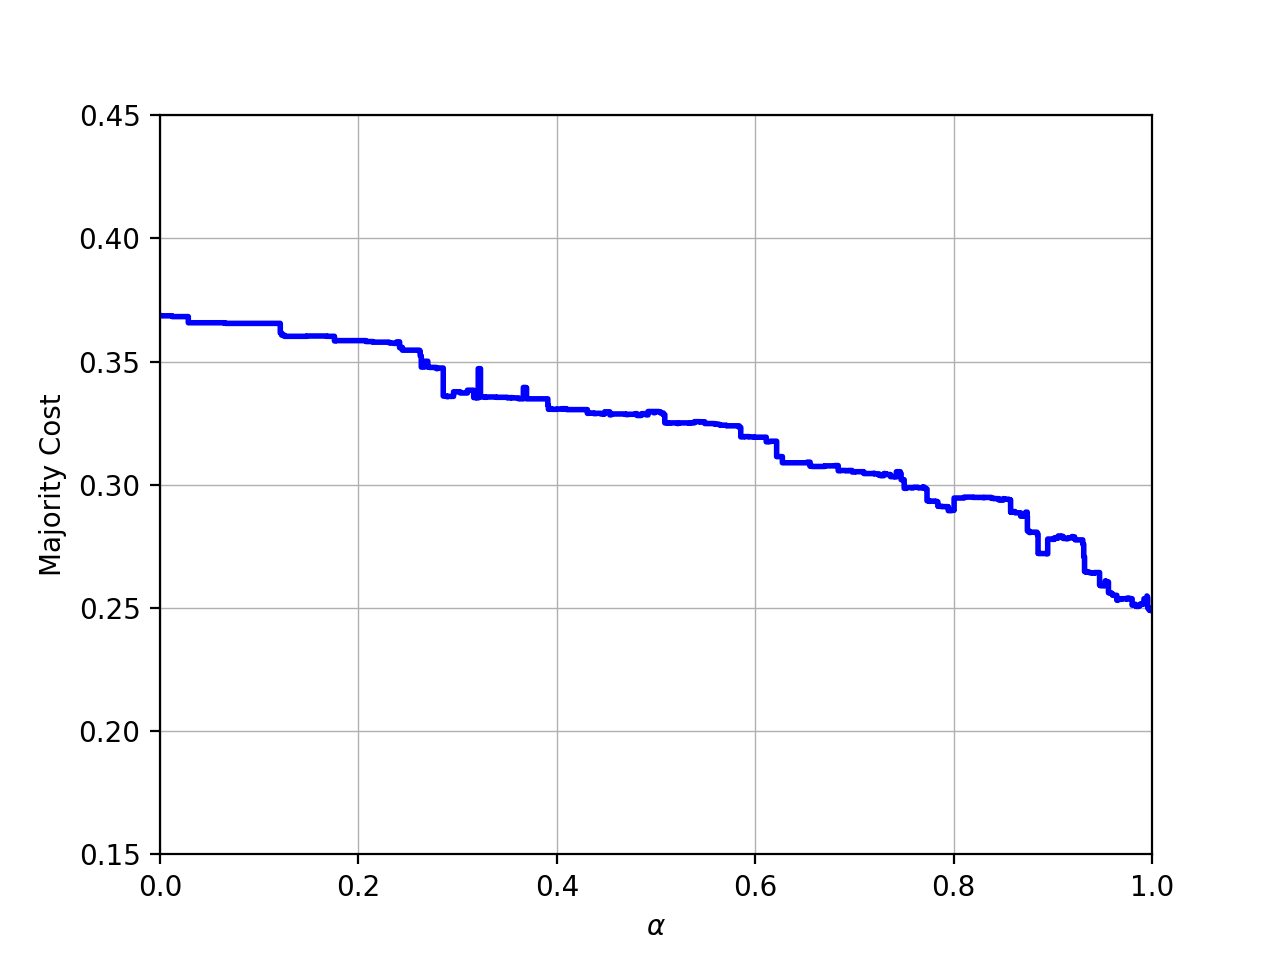
\includegraphics[width=\linewidth]{plots/nell_sa}
\end{minipage}
\begin{minipage}{.3\textwidth}
  \centering
  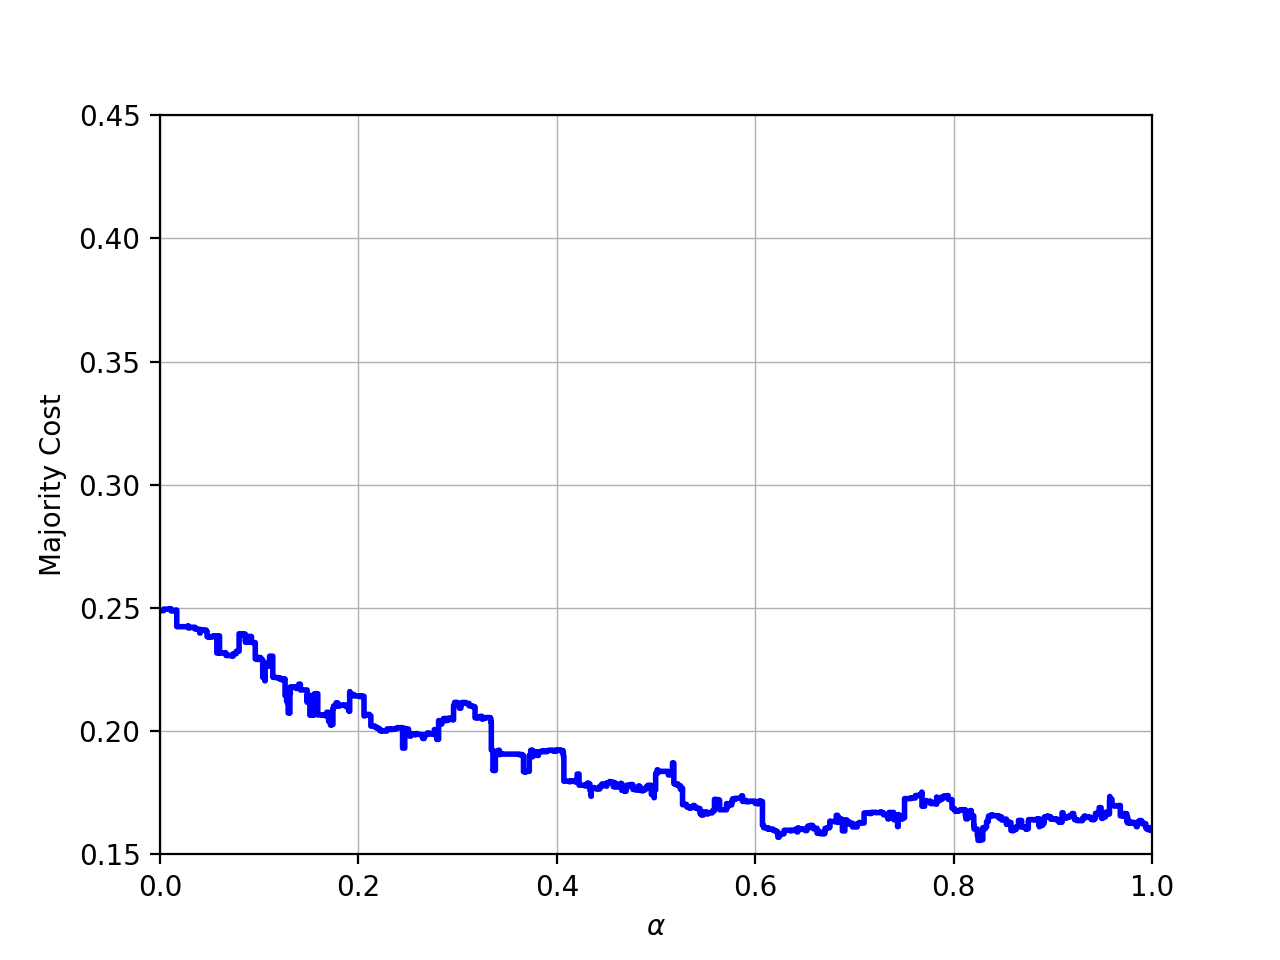
\includegraphics[width=\linewidth]{plots/nell_ac}
\end{minipage}
\caption{$\alpha$-linkage using 250 points for each clustering instance gives minor improvements for the NELL data when clustering between single and complete (left) and average and complete linkage (right). As complete linkage performs best of our input strategies, interpolating between single and average linkage (middle) does not lead to improvements.}
\label{fig:nellresults}
\end{figure}

We see minor improvements when clustering between single and complete and average and complete linkage. On the other hand, interpolating between single and average linkage did not lead to any improvement. In order to evaluate the results further, we have a closer look at the curves and see that the overall improvement we get is $0.53\%$, a reduction from $15.9725\%$ (complete linkage) to $15.4422\%$ ($\alpha_{SC}(0.826)$) as shown in table \ref{table:nellresults}. An interesting observation is that while single linkage performs very poor overall, interpolating between single and complete linkage gives a better improvement than interpolating between average and complete linkage. To evaluate these experiments we are using the Majority Distance, as for such a large number of target clusters calculating the Hamming distance is not efficient. 

\begin{table}[h]
    \centering
    \begin{tabular}{|l | l|}
    \hline
    Strategy & Majority Cost\\ \hline
    Single Linkage & 0.36871\\
    Average Linkage & 0.248913\\
    Complete Linkage & 0.159725\\
    \cellcolor{green!50}$\alpha_{SC}(0.826)$ & \cellcolor{green!50}0.154422\\
    $\alpha_{AC}(0.826)$ & 0.155697\\\hline
    \end{tabular}
    \caption{Our proposed algorithm reduces the NELL cost by $\Delta cost = 0.53\%$ when using a maximum of 250 points for each class.}
    \label{table:nellresults}
\end{table}

As the algorithm became a lot more efficient during this work, we scaled up the algorithms to use 1,000 instead of 250 points per class. Figure \ref{fig:nellresults1000} shows that in general the error is slightly higher. This is because our experiments contain more different classes. Overall, we again see slight improvements that are shown in table \ref{table:nell1000}. Compared to the previous experiments, the improvements were a bit bigger ($1.2078\%$ leading to an error of $16.6742\%$), however the overall curves look very similar. In this setting, we also evaluated the parameter advising for the first 10 parameters $\alpha^*$ (see figure \ref{fig:nell1000top10}).

\begin{figure}[h]
\centering
\begin{minipage}{.45\textwidth}
  \centering
  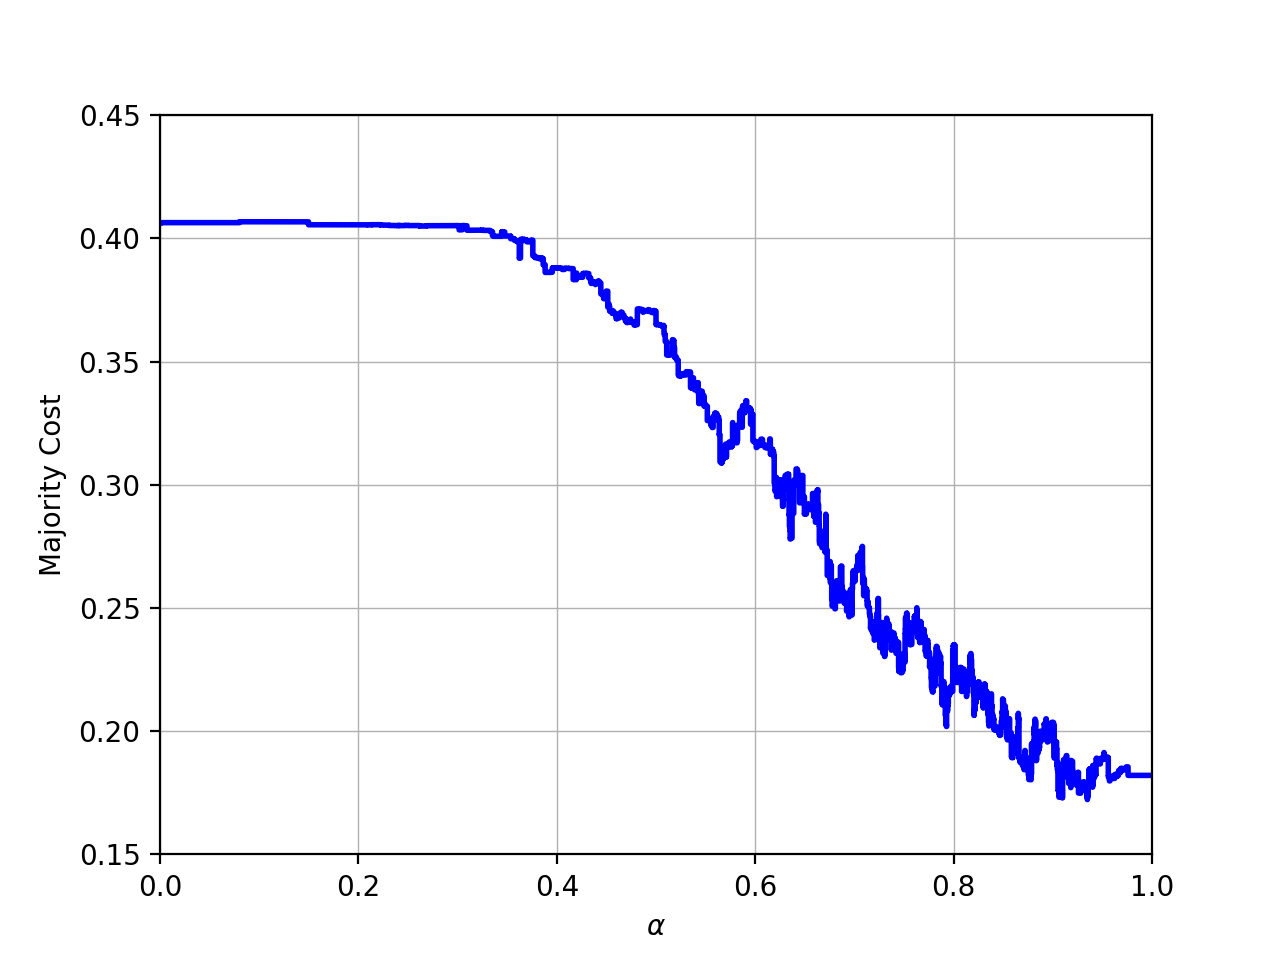
\includegraphics[width=\linewidth]{plots/nell_sc_1000}
\end{minipage}
\begin{minipage}{.45\textwidth}
  \centering
  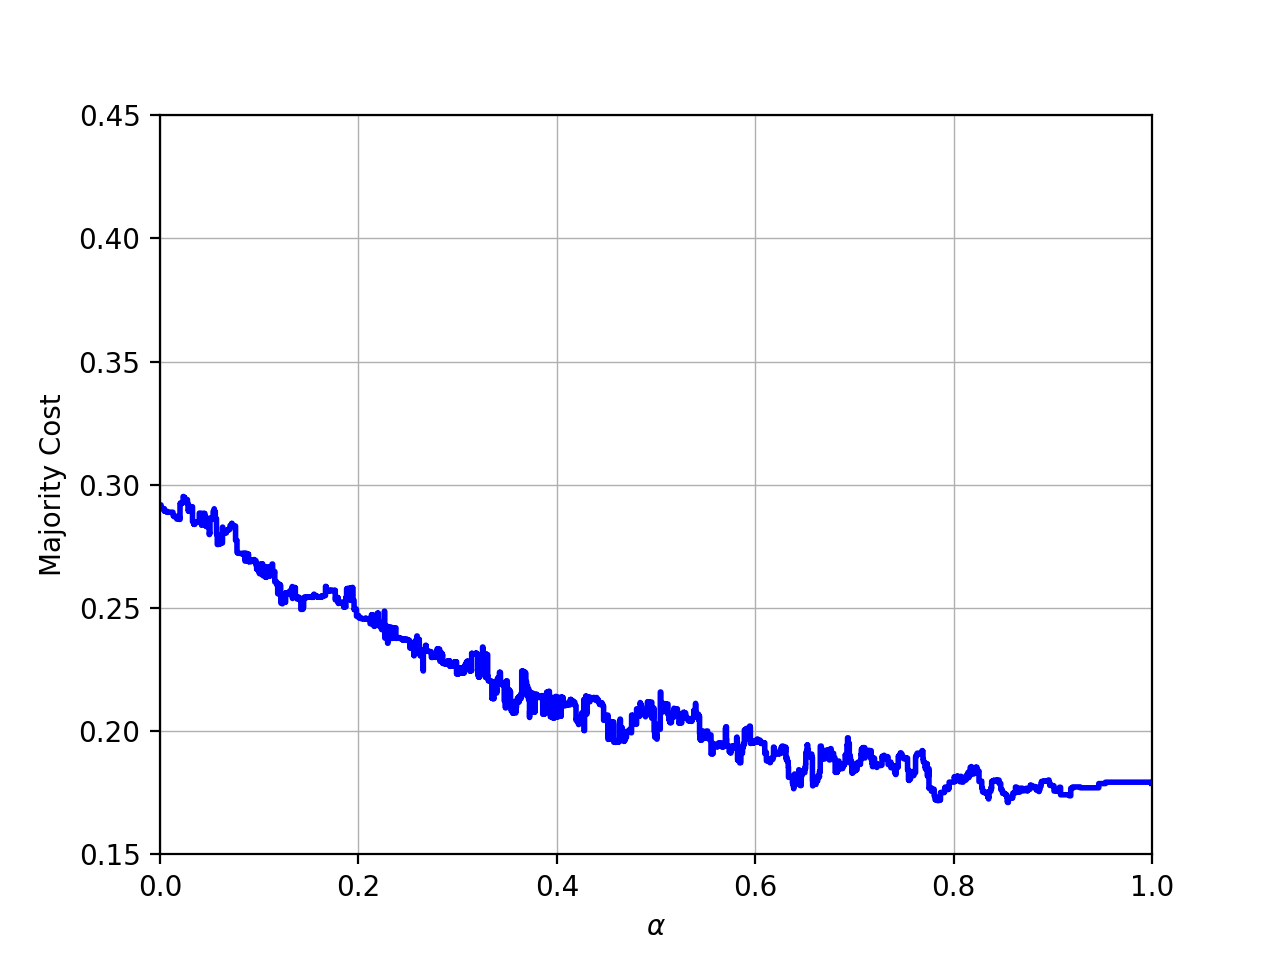
\includegraphics[width=\linewidth]{plots/nell_ac_1000}
\end{minipage}
\caption{$\alpha$-linkage using 1000 points for each clustering instance gives minor improvements for the NELL data when clustering between single and complete (left) and average and complete linkage (right).}
\label{fig:nellresults1000}
\end{figure}

\begin{table}[h]
    \centering
    \begin{tabular}{|l | l|}
    \hline
    Strategy & Majority Cost\\ \hline
    Single Linkage & 0.36871\\
    Average Linkage & 0.291202\\
    Complete Linkage & 0.17882\\
    \cellcolor{green!50}$\alpha_{SC}(0.918)$ & \cellcolor{green!50}0.166742\\
    $\alpha_{AC}(0.855)$ & 0.171083\\\hline
    \end{tabular}
    \caption{Our proposed algorithm reduces the NELL cost by $\Delta cost = 1.2078\%$ when using a maximum of 1000 points for each class.}
    \label{table:nell1000}
\end{table}

\begin{figure}[h]
\centering
\begin{minipage}{.45\textwidth}
  \centering
  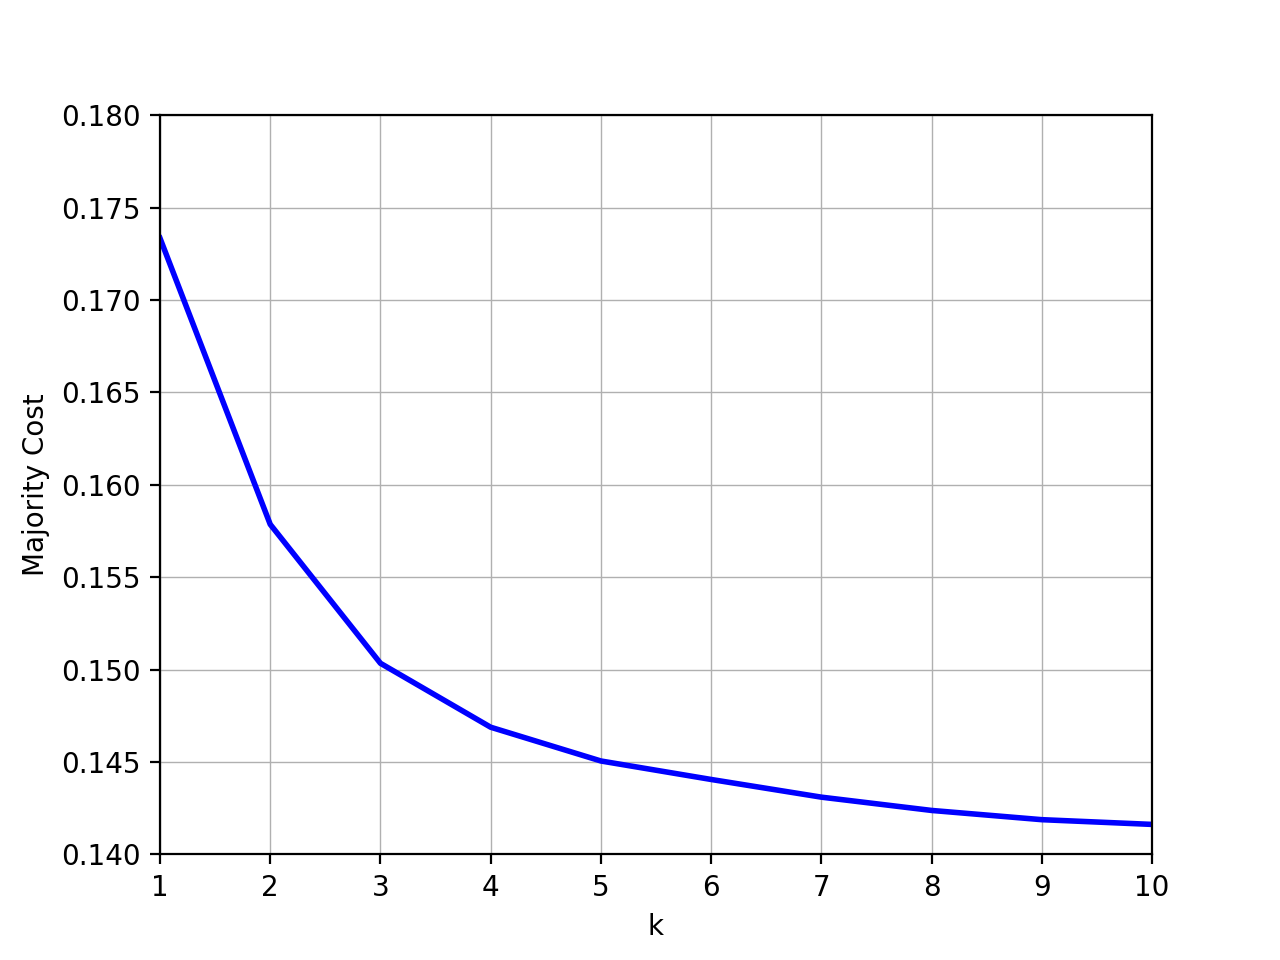
\includegraphics[width=\linewidth]{plots/nell_sc_1000_top10}
\end{minipage}
\begin{minipage}{.45\textwidth}
  \centering
  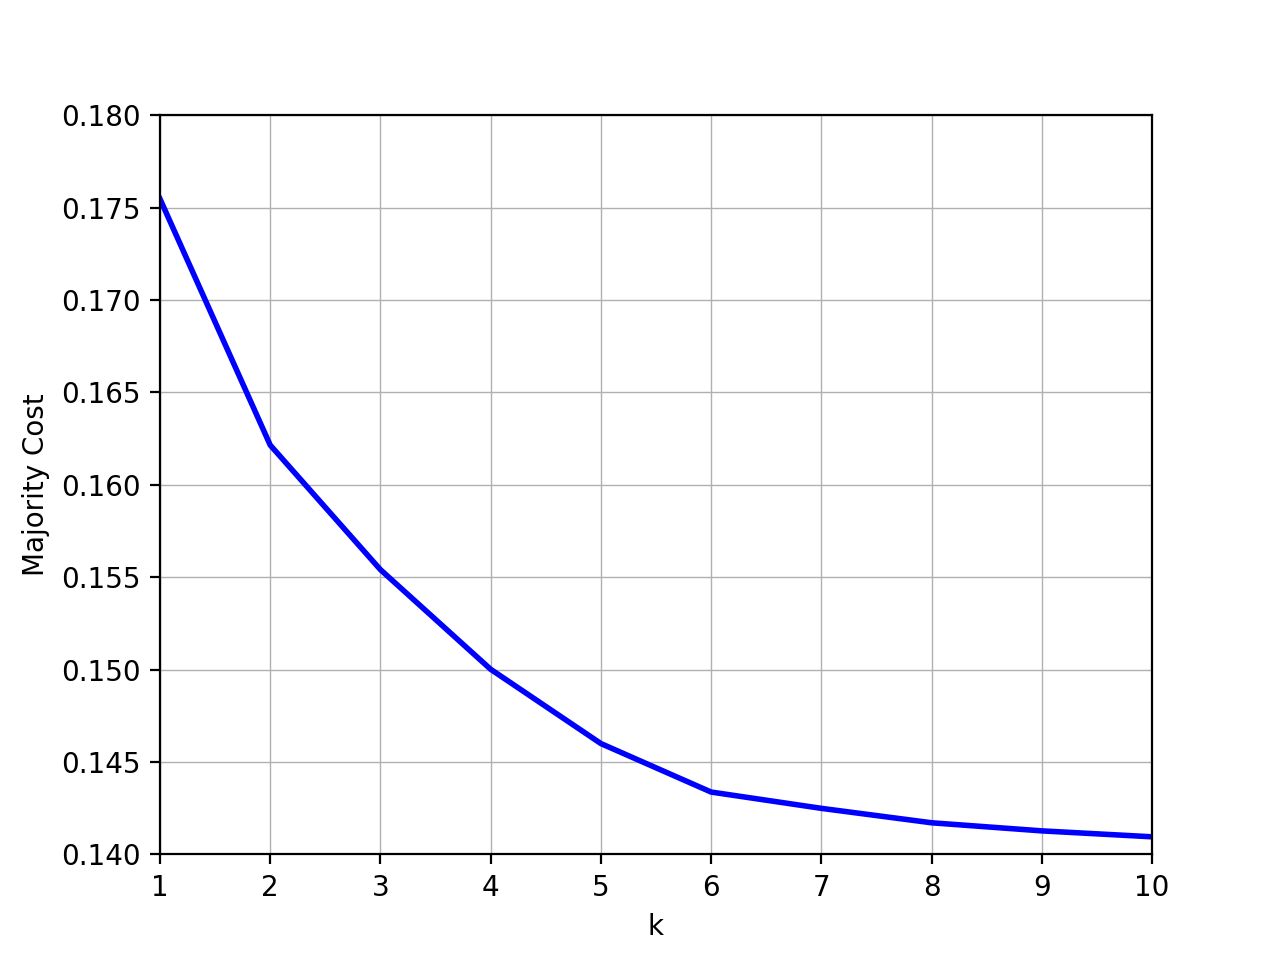
\includegraphics[width=\linewidth]{plots/nell_ac_1000_top10}
\end{minipage}
\caption{$\alpha$-linkage using 1000 points for each clustering instance gives minor improvements for the NELL data when clustering between single and complete (left) and average and complete linkage (right).}
\label{fig:nell1000top10}
\end{figure}

Also, we evaluated the corresponding clusters. As $\alpha$-linkage uses agglomerative hierarchical clustering, we can extract clusters at different levels starting with each noun phrase as its own cluster. Tables \ref{tbl:rooms}, \ref{tbl:clothing} and \ref{tbl:kitchenitems} show some examples for discovered categories.

\begin{table}[H]
  \makebox[\textwidth][c]{
  \small
  \begin{tabular}{cccc}
    \hline\hline
    \textbf{Luxury Room} & \textbf{Bathroom} & \textbf{Guest Room} & \textbf{Suite} \\ \hline
    spacious living room & large ensuite bathroom & elegant rooms & luxurious suites\\
    comfortable living room & spacious marble bathroom & three guest rooms & one bedroom suites\\
    guest room & one bathroom & large guest rooms & spacious suites\\
    lounge room & full bathroom & deluxe guest rooms & deluxe suites\\
    living room & upstairs bathroom & guests rooms & guest suites\\
    superior room & large bathroom & spacious air conditioned rooms & bedroom suites\\
    sleeping room & ensuite bathroom & furnished guest rooms & whirlpool suites\\
    main bedroom & elegant bathroom & comfortable guest rooms & three suites\\
    \hline
  \end{tabular}
  }
  \caption{Proposed Subcategories for ``Office Building Room''.}
  \label{tbl:rooms}
\end{table}

\begin{table}[H]
  \makebox[\textwidth][c]{
  \small
  \begin{tabular}{ccccc}
    \hline\hline
    \textbf{Shoes} & \textbf{Uniform/Costume} & \textbf{Pants} & \textbf{Casual} & \textbf{Specialized} \\ \hline
    shoes & costume & kneepants & stocking cap & long stockings\\
    high heel shoes & work uniforms & baggy pants & workout clothes & wide brimmed hat\\
    sensible shoes & outfits & loose fitting pants & casual clothes & casual wear\\
    old shoes & period costume & slacks & baseball caps & black stockings\\
    pointe shoes & folk costumes & black shorts & skull caps & wear socks\\
    dark shoes & halter top & special clothing & ball caps & high heels\\
    spira shoes & period costumes & white shorts & evening clothes & surf wear\\
    mens shoes & costumes & underpants & ball cap & wear gloves\\
    \hline
  \end{tabular}
  }
  \caption{Proposed Subcategories for ``Clothing''.}
  \label{tbl:clothing}
\end{table}

\begin{table}[H]
  \makebox[\textwidth][c]{
  \small
  \begin{tabular}{cccc}
    \hline\hline
    \textbf{Stove/Oven} & \textbf{Machines} & \textbf{Bowls} & \textbf{Baking Sheets} \\ \hline
    full size stove & cookie cutters & large mixing bowl & oiled baking sheet\\
    full size cooker & automatic washing machine & large serving bowl & rimmed baking sheet\\
    red hot stove & washing machine & small bowl & large baking sheet\\
    plastic jug & bread machine & single bowl & small baking sheet\\
    toaster & cookie cutter & separate bowl & prepared baking sheet\\
    greased baking dish & coffee machine & shallow bowl & ungreased baking sheet\\
    wood burning pizza oven & cooking spray & separate mixing bowl & hot plate\\
    ceramic top stove & coffee grinder & large bowl & greased baking sheet\\
    \hline
  \end{tabular}
  }
  \caption{Proposed Subcategories for ``Kitchen Item''.}
  \label{tbl:kitchenitems}
\end{table}

In addition to using the original features, we also use the word embeddings and the bag-of-contexts representations to evaluate these experiments.

\todo[inline]{Add experiments for new features.}

\paragraph{MNIST Experiments.} For the MNIST images, we evaluate both describes experimental settings with combinations of five out of the ten target classes. In addition to using the raw pixel features. To cluster the data, we set up $10 \choose 5$ $= 252$ different experiments by selecting all combinations of five out of the ten labels. In order to do so in efficient time, we subsample the dataset to 200 points for each label, so one experiment will cluster 1000 points. First, we evaluated the results for both average to complete and single to complete linkage for several batches. Note that we do not discuss the interpolation between single to average linkage in this and the following paragraphs, as experiments did not lead to improvements. First, we show the experiments for the six first batches $b_i, i \in \{0, 1, 2, 3, 4, 5\}$ for interpolating between single and complete linkage.

\begin{figure}[h]
\centering
\begin{minipage}{.3\textwidth}
  \centering
  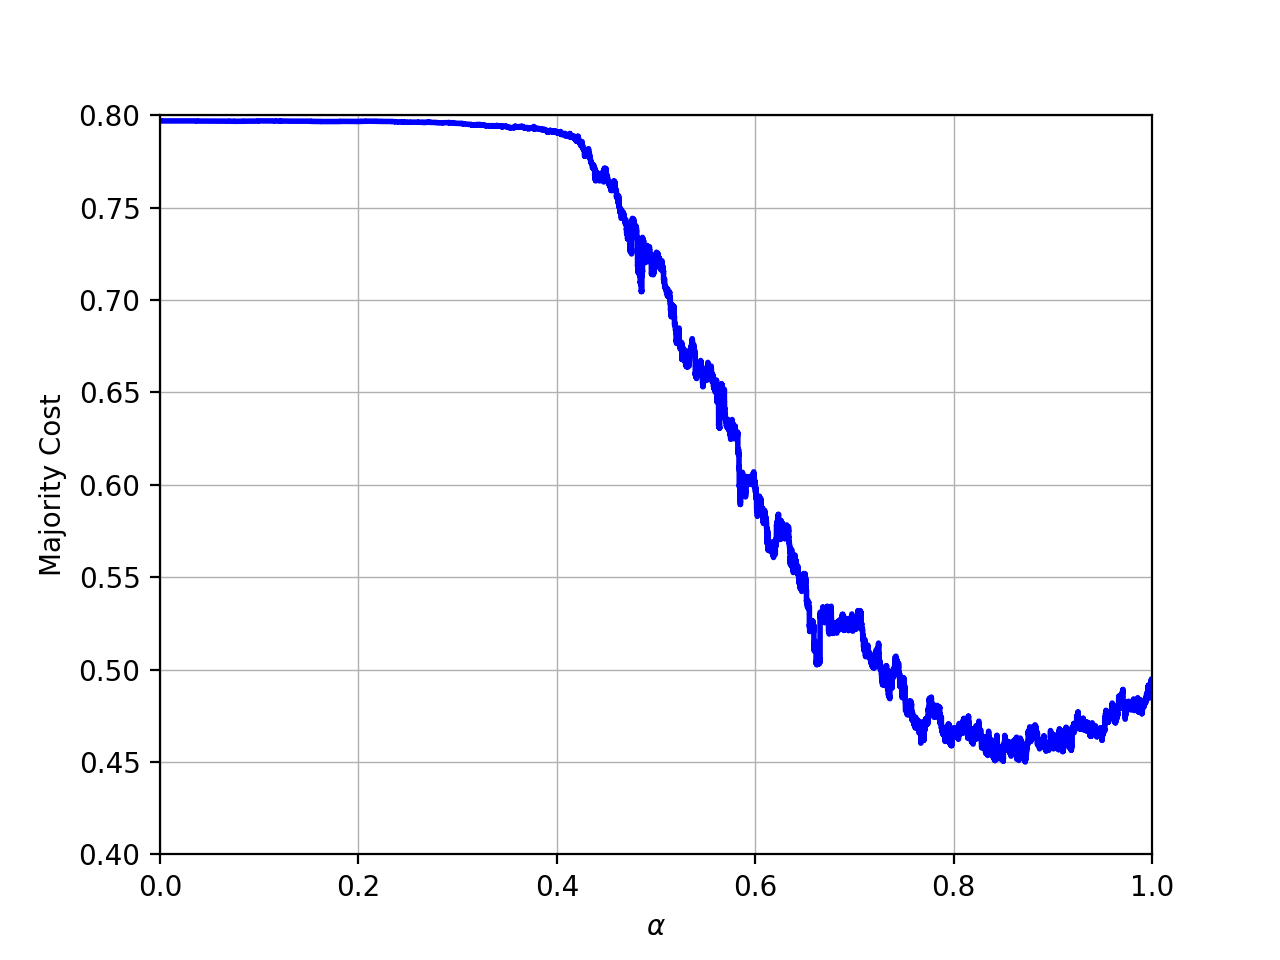
\includegraphics[width=\linewidth]{plots/mnist-sc-0}
\end{minipage}
\begin{minipage}{.3\textwidth}
  \centering
  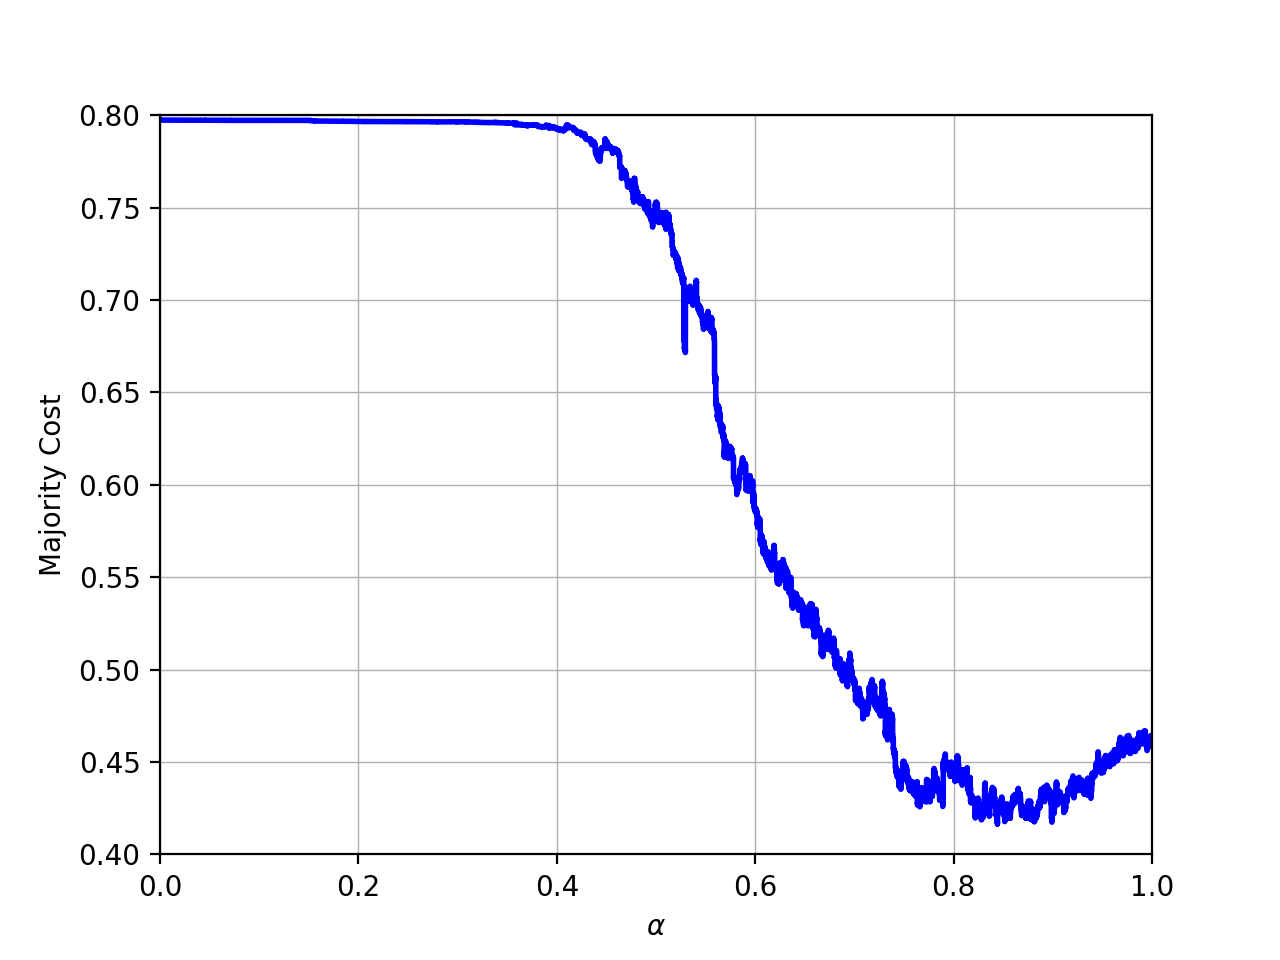
\includegraphics[width=\linewidth]{plots/mnist-sc-1}
\end{minipage}
\begin{minipage}{.3\textwidth}
  \centering
  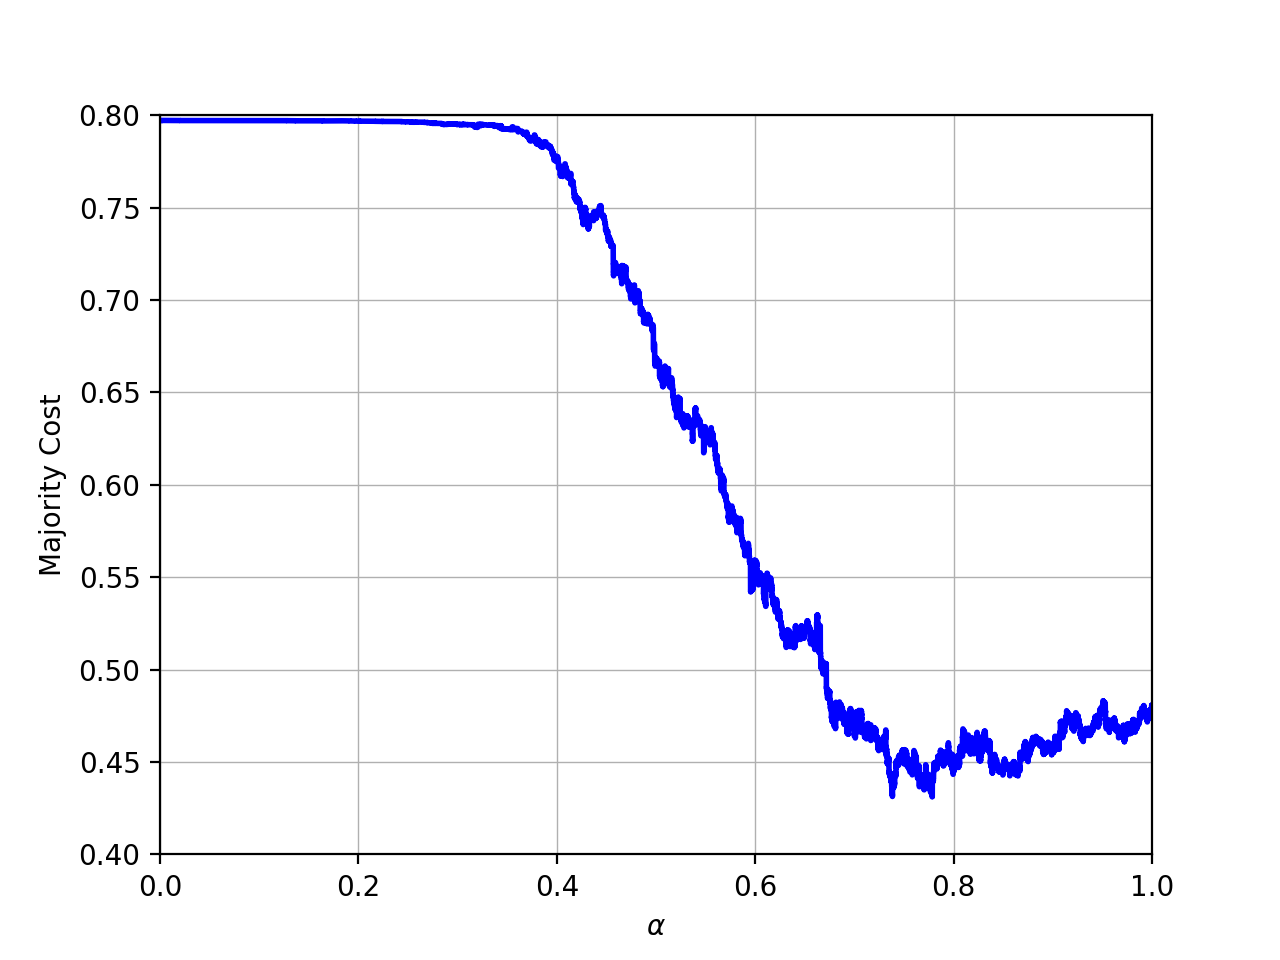
\includegraphics[width=\linewidth]{plots/mnist-sc-2}
\end{minipage}
\begin{minipage}{.3\textwidth}
  \centering
  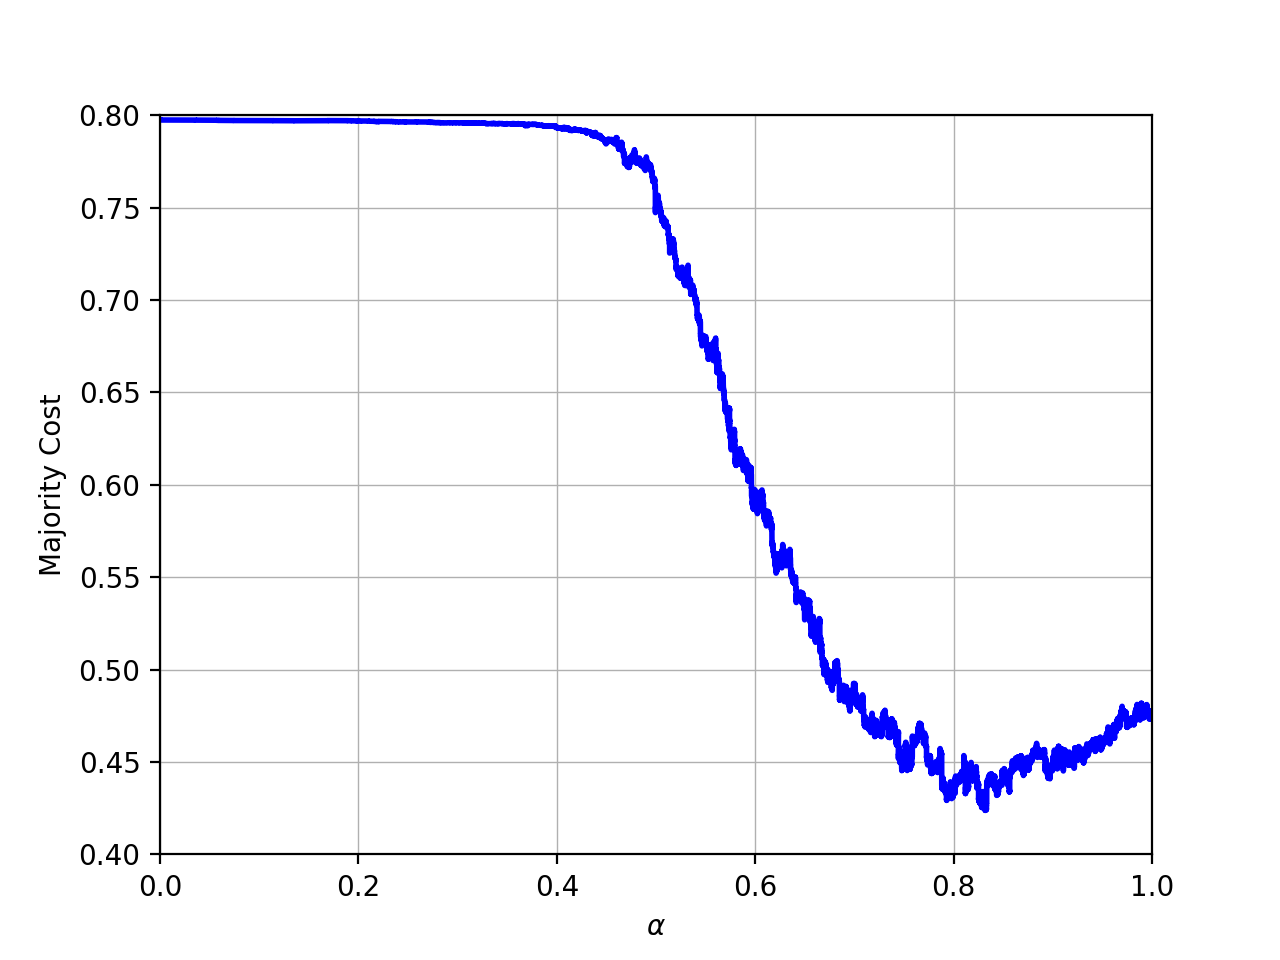
\includegraphics[width=\linewidth]{plots/mnist-sc-3}
\end{minipage}
\begin{minipage}{.3\textwidth}
  \centering
  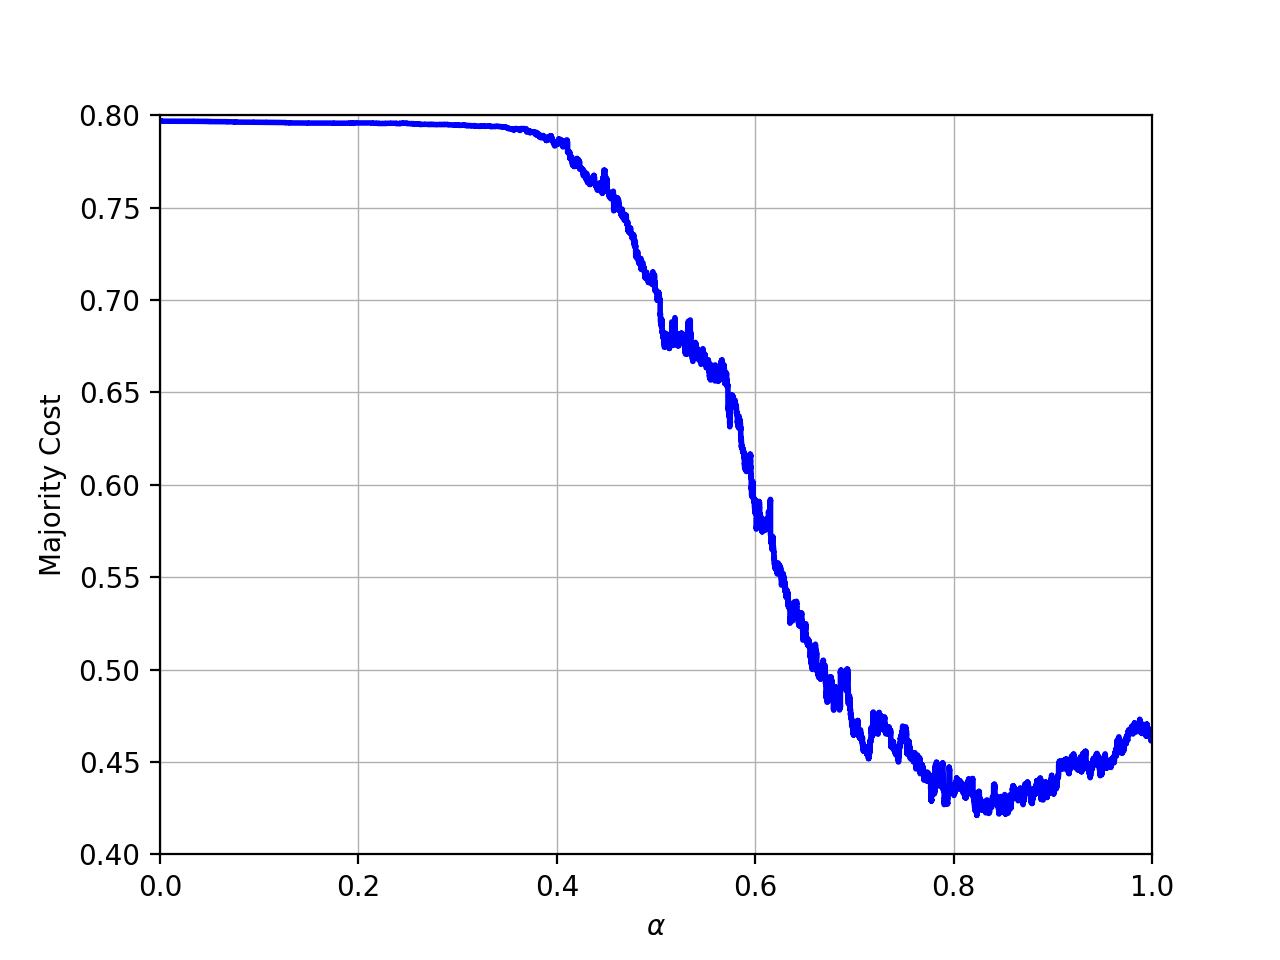
\includegraphics[width=\linewidth]{plots/mnist-sc-4}
\end{minipage}
\begin{minipage}{.3\textwidth}
  \centering
  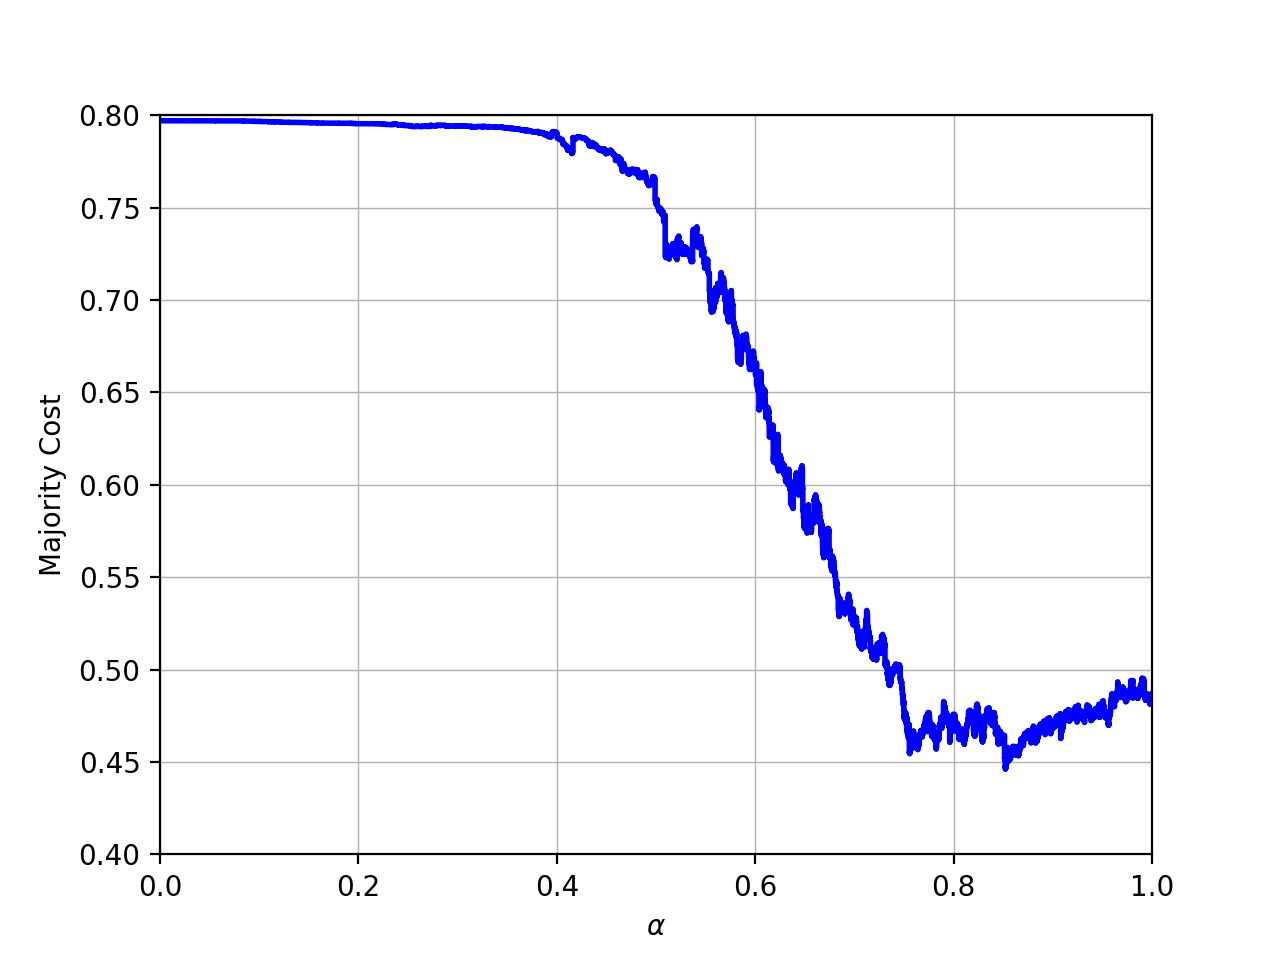
\includegraphics[width=\linewidth]{plots/mnist-sc-5}
\end{minipage}
\caption{Over the first six batches of the MNIST data, interpolating between single and complete linkage shows a similar behavior.}
\label{fig:mnistscbatches}
\end{figure}

As shown in figure \ref{fig:mnistscbatches}, the clustering over the first six batches leads to very similar curves with slightly different errors. Table \ref{table:mnistscbatches} evaluates the results in more detail.

\begin{table}[H]
    \centering
    \begin{tabular}{|l | l l l l l l |}
    \hline
    Strategy & Batch 0 & Batch 1 & Batch 2 & Batch 3 & Batch 4 & Batch 5\\ \hline
    Single Linkage & 0.796901 & 0.797345 & 0.797171 & 0.797405 & 0.796766 & 0.797024\\
    Complete Linkage & 0.490468 & 0.461063 & 0.479825 & 0.475329 & 0.463321 & 0.487111\\
    $\alpha_{opt}$ & 0.87228 & 0.84419 & 0.778498 & 0.83199 & 0.82338 & 0.852251\\
    $cost_{opt}$ & 0.450012 & 0.416433 & 0.431143 & 0.423786 & 0.421103 & 0.446032\\
    $\Delta cost$ & 4.0456\% & 4.463\% & 4.8682\% & 5.1543\% & 4.2218\% & 4.1079\%\\\hline
    \end{tabular}
    \caption{$\alpha$-linkage reduces the cost of the MNIST dataset by up to $\Delta_{max} cost = 5.1543\%$ when interpolating between single and complete linkage.}
    \label{table:mnistscbatches}
\end{table}

Table \ref{table:mnistscbatches} leads to several observations. Clustering points of five classes with a random guess will result in an error of $80\%$. As for all batches single linkage results in an error between $79\%$ and $80\%$, we note that single linkage performs similar than a random guess would. Thus, single linkage is not suitable for the MNIST data. In comparison, complete linkage results in errors below $50\%$ on just using the pixel data. It is not necessarily a great result, but it indicates that grouping high-dimensional pixel features with unsupervised learning can work. Also, we note that the parameter $\alpha_{opt}$ doesn't vary that much and also we notice in figure \ref{fig:mnistscbatches} that for $\alpha \in [0.75,1.0)$ we outperform complete linkage in all cases. As the results are very similar for the used batches, we also average over the batches in figure \ref{fig:mnistscbatchesavg}.

\begin{figure}[h]
    \centering
    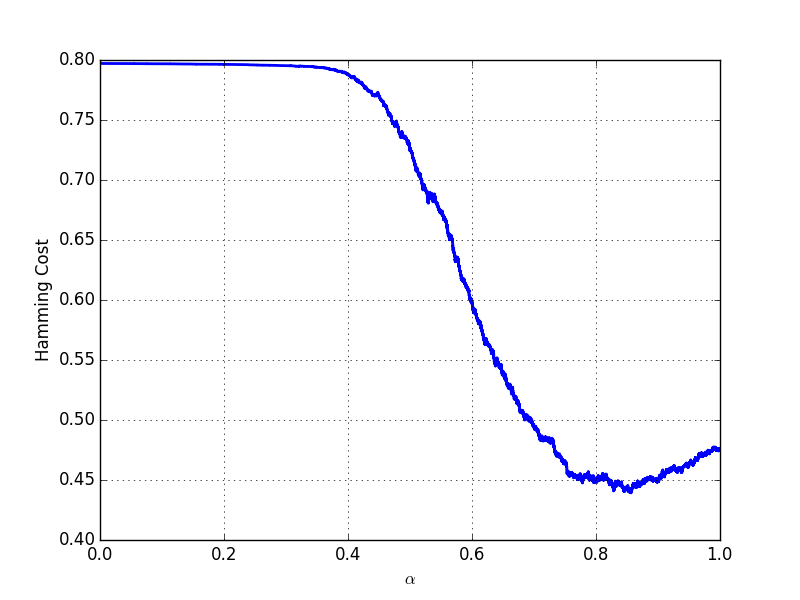
\includegraphics[width=0.5\textwidth]{plots/mnist-sc-averaged.png}
    \caption{Evaluating the first six batches of the MNIST data interpolating between single and complete linkage results in major improvements over both single and complete linkage.}
    \label{fig:mnistscbatchesavg}
\end{figure}

\begin{table}[H]
    \centering
    \begin{tabular}{|l | l |}
    \hline
    Strategy & Hamming Cost\\ \hline
    Single Linkage & 0.797102\\
    Complete Linkage & 0.476186\\
    $\alpha_{opt}$ & 0.857\\
    $cost_{opt}$ & 0.439207\\
    $\Delta cost$ & 3.6979\%\\\hline
    \end{tabular}
    \caption{Over the first 12,000 points of the MNIST dataset interpolating between single and complete linkage improves hamming cost by $3.7\%$ }
    \label{table:mnist1000avgsc}
\end{table}

Figure \ref{fig:mnistscbatchesavg} and table \ref{table:mnist1000avgsc} show that by applying $\alpha$-linkage interpolating between single and complete linkage we improve the hamming cost by $3.7\%$ over the first six data batches, i.e. the first 12,000 points of the dataset. Next, we evaluate the randomized experiments for the same interpolation method, where we average over 512 experiments that are run with random label subsets and randomly selected points for each of the selected labels. Figure \ref{fig:mnistscrandom} shows that in this setting we obtain a very similar curve as in the other setting (figure \ref{fig:mnistscbatchesavg}).

\begin{figure}[h]
    \centering
    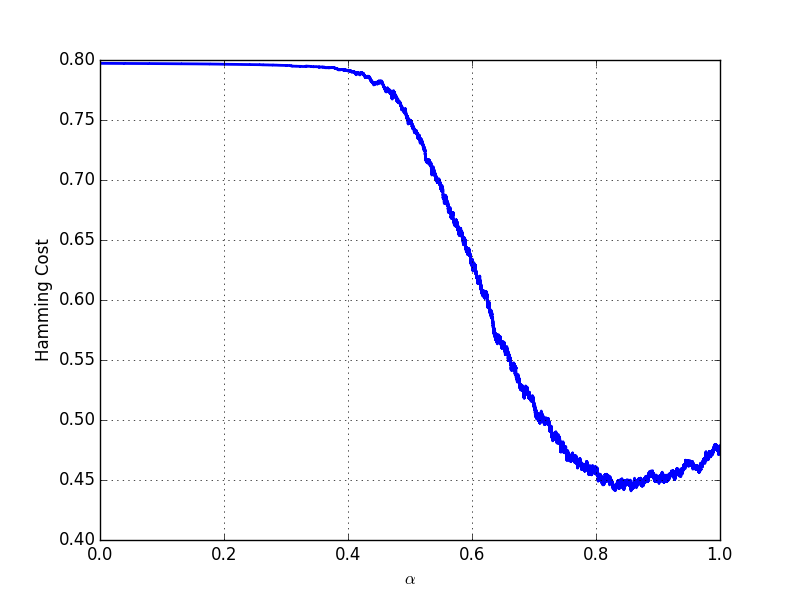
\includegraphics[width=0.5\textwidth]{plots/mnist-sc-random.png}
    \caption{Selecting labels and points randomly leads to a similar curve when interpolating between single and complete linkage using the MNIST data.}
    \label{fig:mnistscrandom}
\end{figure}

\begin{table}[H]
    \centering
    \begin{tabular}{|l | l | l |}
    \hline
    Strategy & Hamming Cost (Batch) & Hamming Cost (Random)\\ \hline
    Single Linkage & 0.797102 & 0.797215\\
    Complete Linkage & 0.476186 & 0.476355\\
    $\alpha_{opt}$ & 0.857 & 0.857\\
    $cost_{opt}$ & 0.439207 & 0.440932\\
    $\Delta cost$ & 3.6979\% & 3.5423\%\\\hline
    \end{tabular}
    \caption{Evaluating the randomized setting leads to exactly the same parameter $\alpha_{opt}$ and a similar cost improvement as in the batch setting for the MNIST data.}
    \label{table:mnist1000randomsc}
\end{table}

Table \ref{table:mnist1000randomsc} compares the results for both settings when interpolating between single and complete linkage. We obtain very similar results for single and complete linkage. Also, the optimal parameter $\alpha_{opt}$ is the same in both settings leading to similar improvements in the hamming cost. This means that $\alpha$-linkage is robust over the entire MNIST distribution and with an improvement of more than $3\%$ towards complete linkage it outperforms both used linkage strategies by a major difference. In addition, we also evaluate the greedy parameter advising for the previous experiments.\\

\begin{figure}[h]
\centering
\begin{minipage}{.45\textwidth}
  \centering
  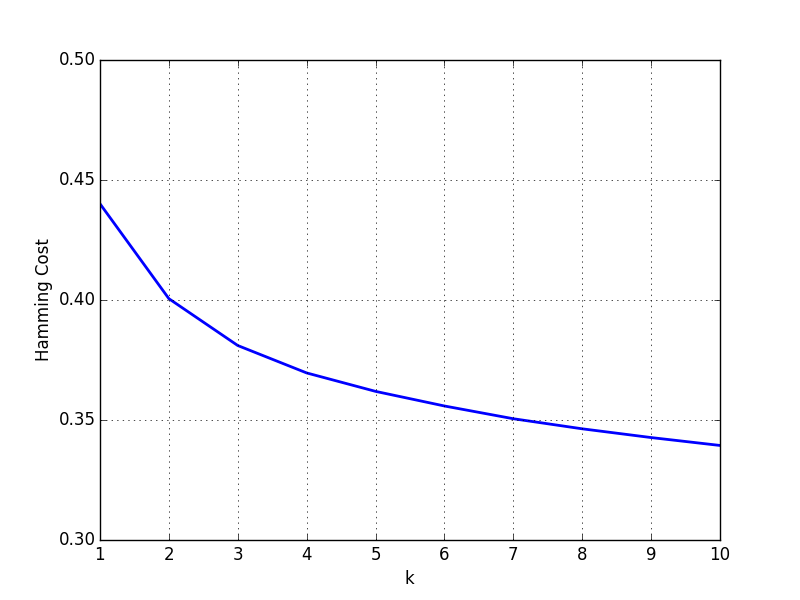
\includegraphics[width=\linewidth]{plots/mnist-sc-top-10}
\end{minipage}
\begin{minipage}{.45\textwidth}
  \centering
  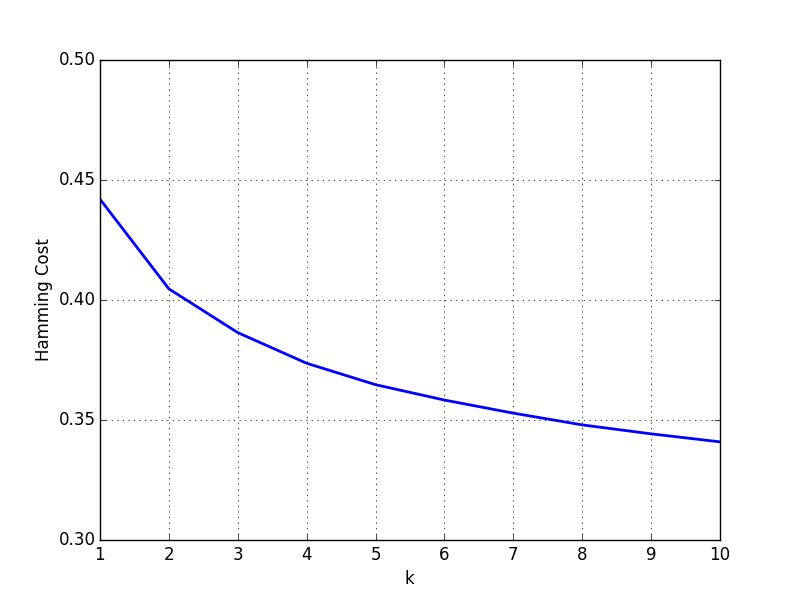
\includegraphics[width=\linewidth]{plots/mnist-sc-random-top-10}
\end{minipage}
\caption{}
\label{fig:mnistsctop10}
\end{figure}

Figure \ref{fig:mnistsctop10} shows that we again obtain very similar results for the batch setting (left) and the random setting (right). By using $k = 3$ parameters $\alpha^*$ the cost drops more than $5\%$ in addition to less than $38\%$. In comparison to the best linkage strategy, i.e. complete linkage, this is an improvement of $\approx 10\%$.\\

Similar to that, we also interpolate between average and complete linkage and evaluate both the batch and the random setting. Figure \ref{fig:mnist1000acbatch} and table \ref{table:mnist1000acbatch} show that the results of the different batches vary much. On the one hand, the parameters $\alpha_{opt}$ have a wider range ($\alpha_{opt} \in [0.53,0.81]$), but on the other hand, we get slightly larger improvements for the hamming cost in comparison to complete linkage.

\begin{figure}[h]
\centering
\begin{minipage}{.3\textwidth}
  \centering
  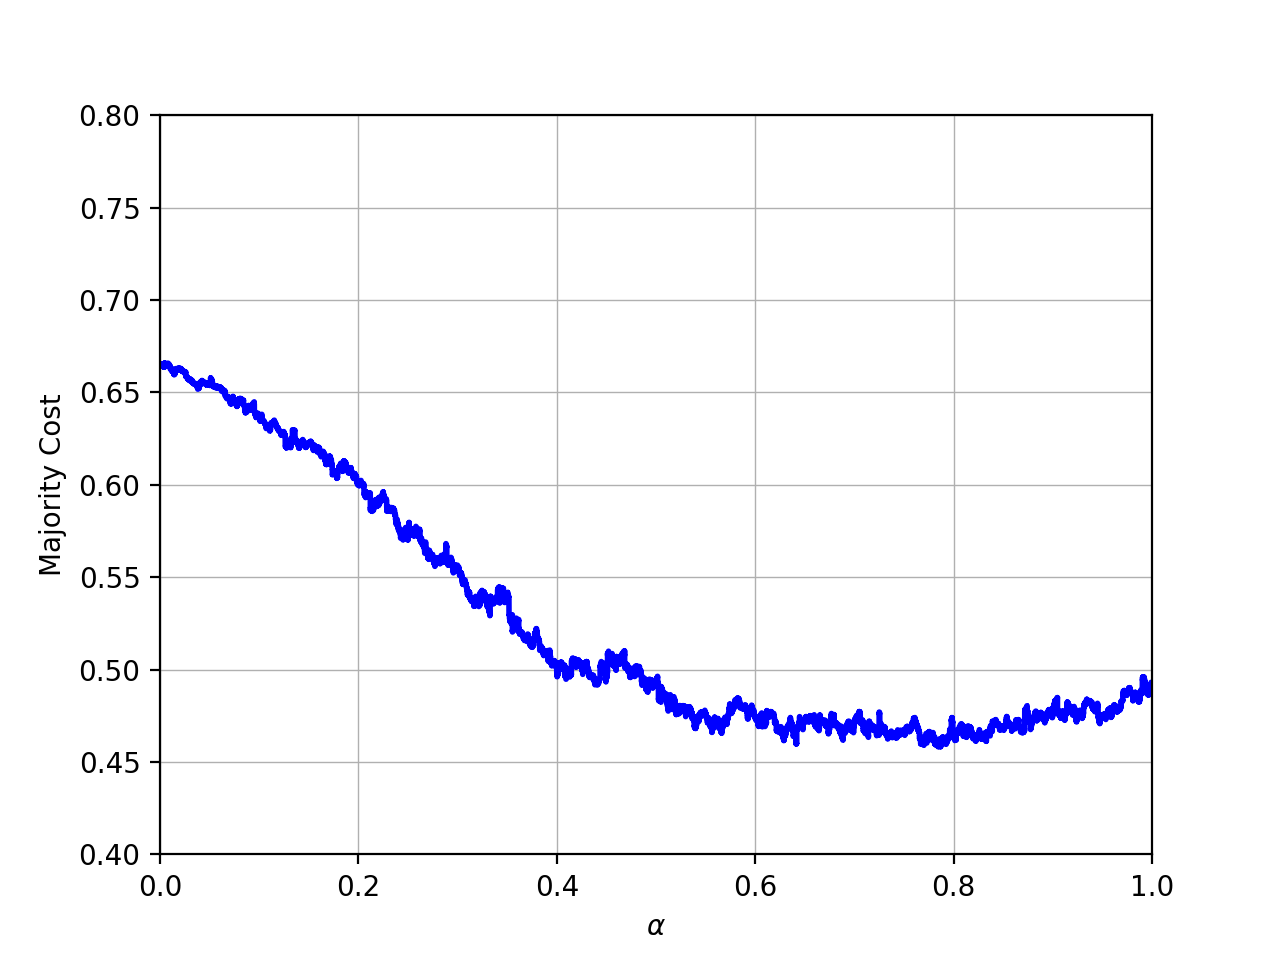
\includegraphics[width=\linewidth]{plots/mnist-ac-0}
\end{minipage}
\begin{minipage}{.3\textwidth}
  \centering
  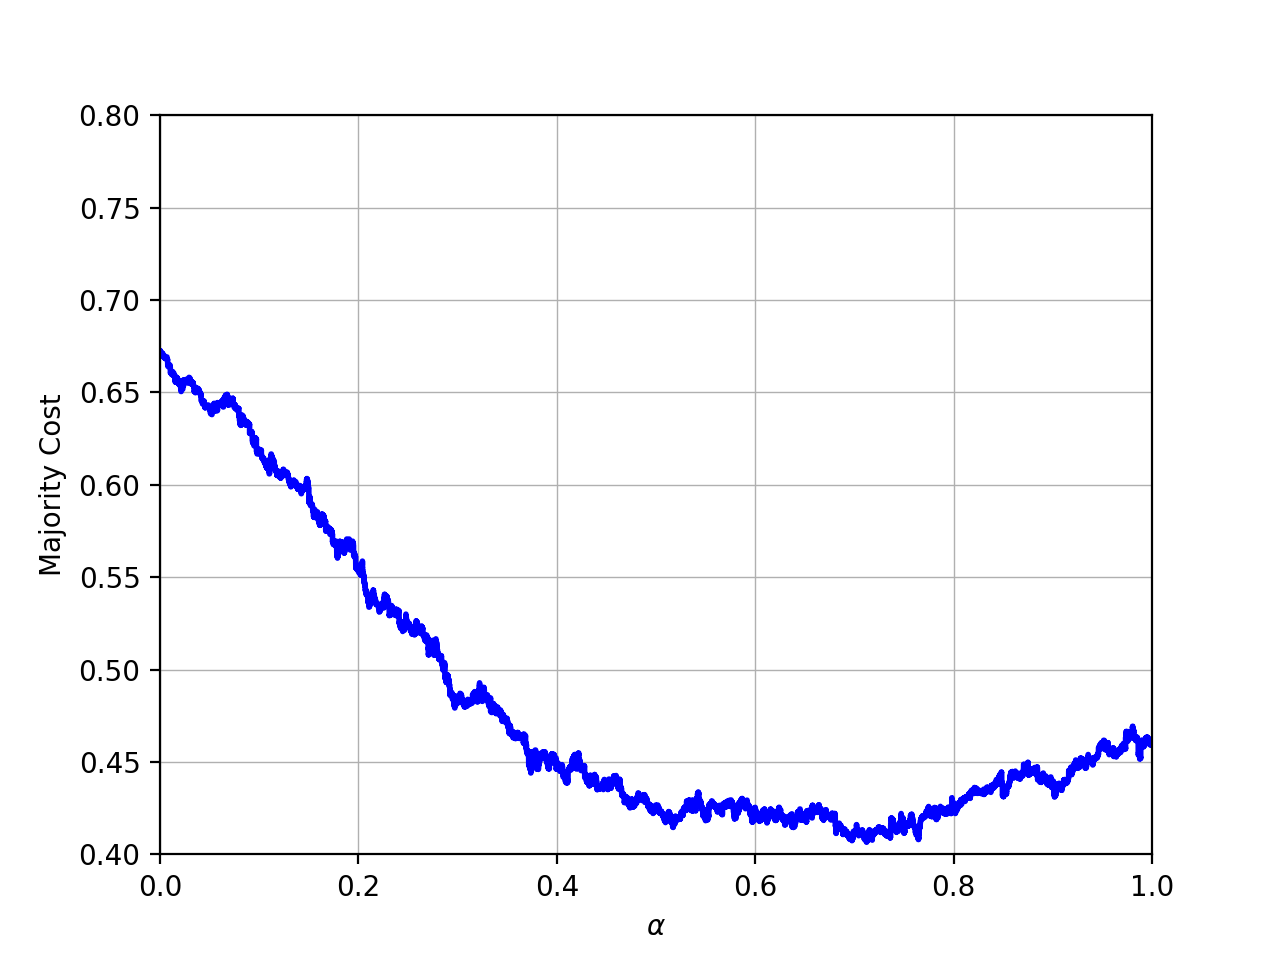
\includegraphics[width=\linewidth]{plots/mnist-ac-1}
\end{minipage}
\begin{minipage}{.3\textwidth}
  \centering
  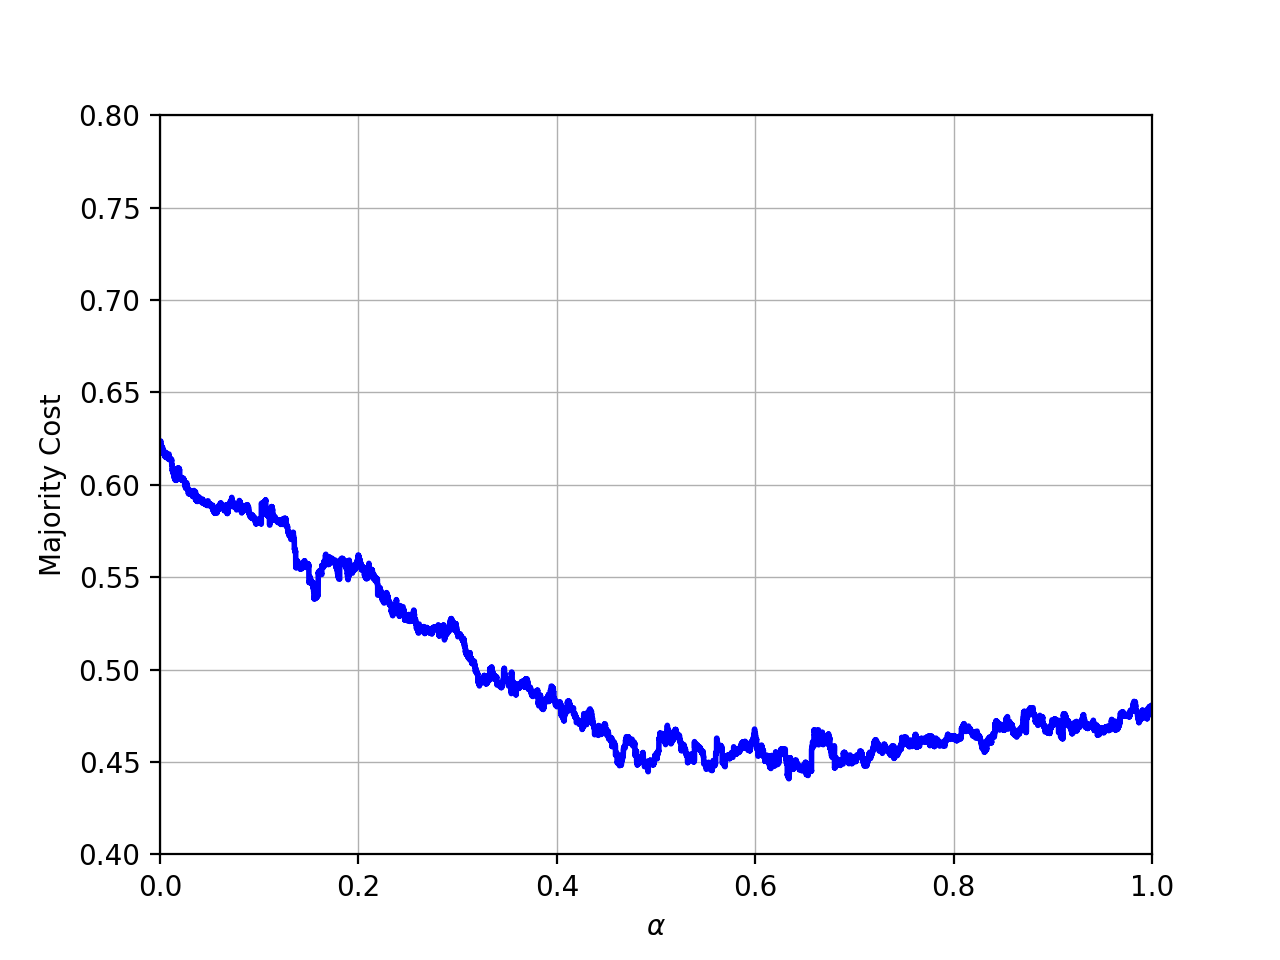
\includegraphics[width=\linewidth]{plots/mnist-ac-2}
\end{minipage}
\begin{minipage}{.3\textwidth}
  \centering
  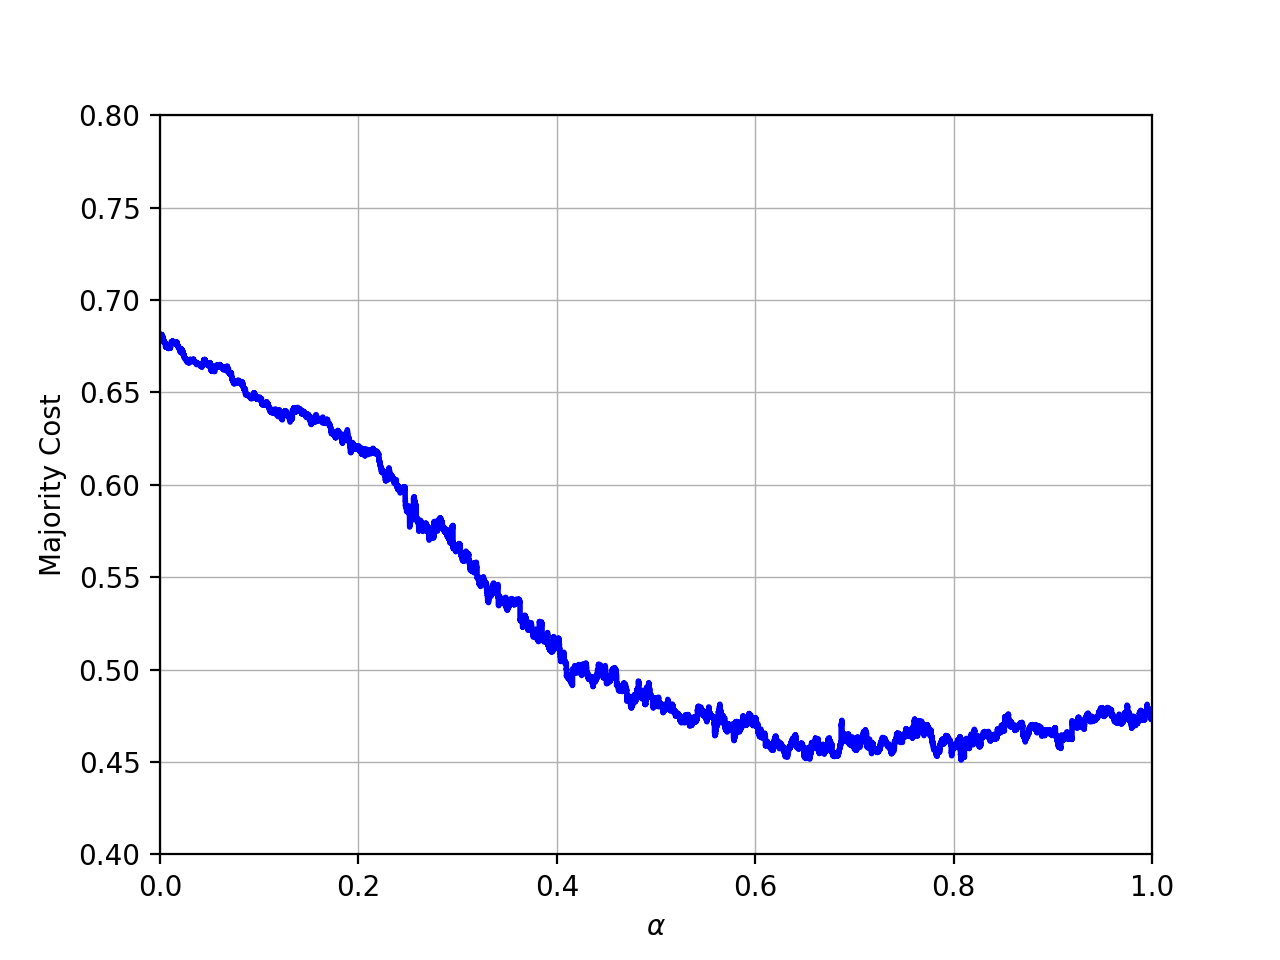
\includegraphics[width=\linewidth]{plots/mnist-ac-3}
\end{minipage}
\begin{minipage}{.3\textwidth}
  \centering
  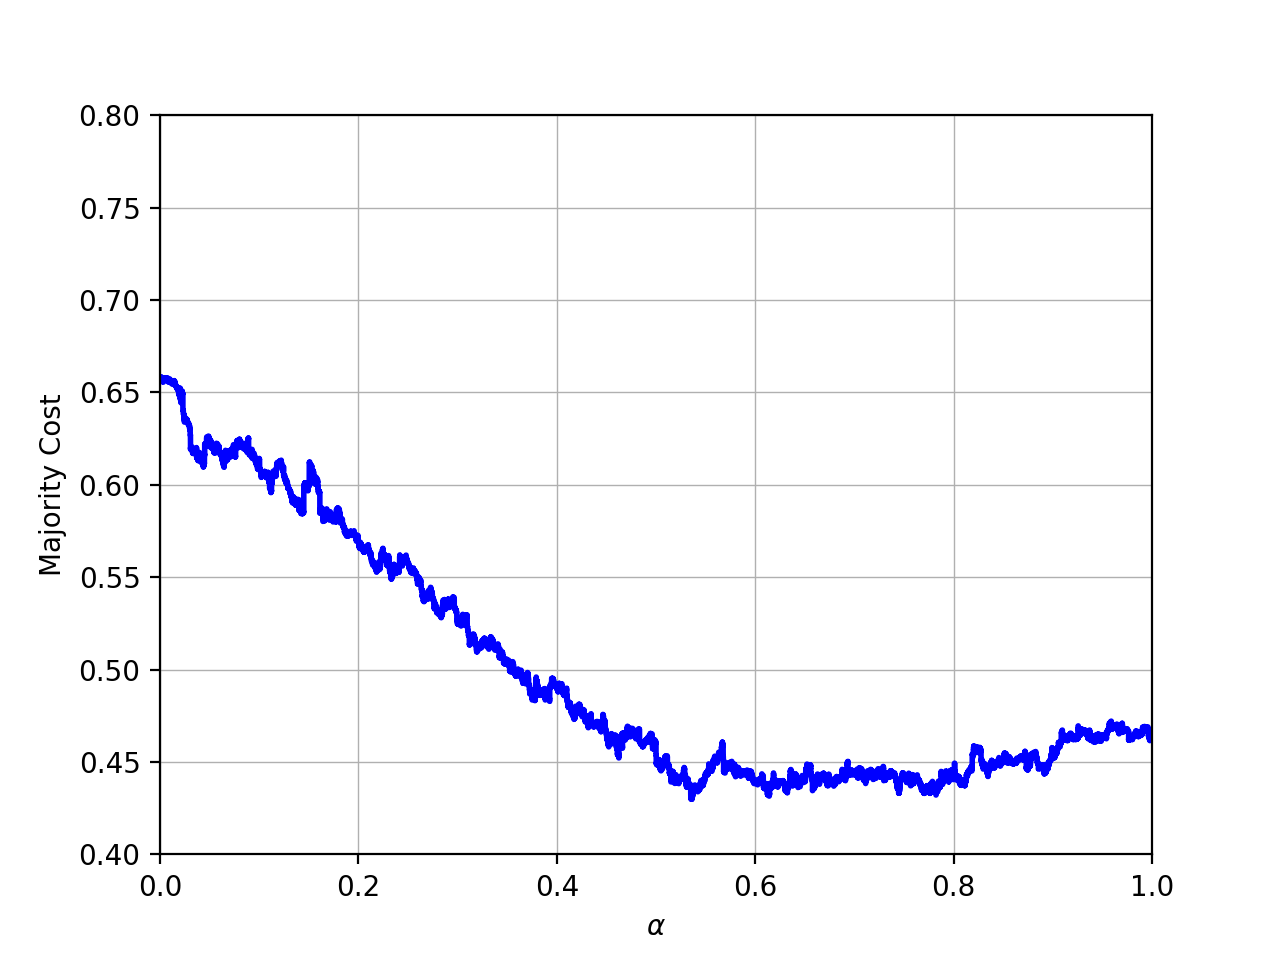
\includegraphics[width=\linewidth]{plots/mnist-ac-4}
\end{minipage}
\begin{minipage}{.3\textwidth}
  \centering
  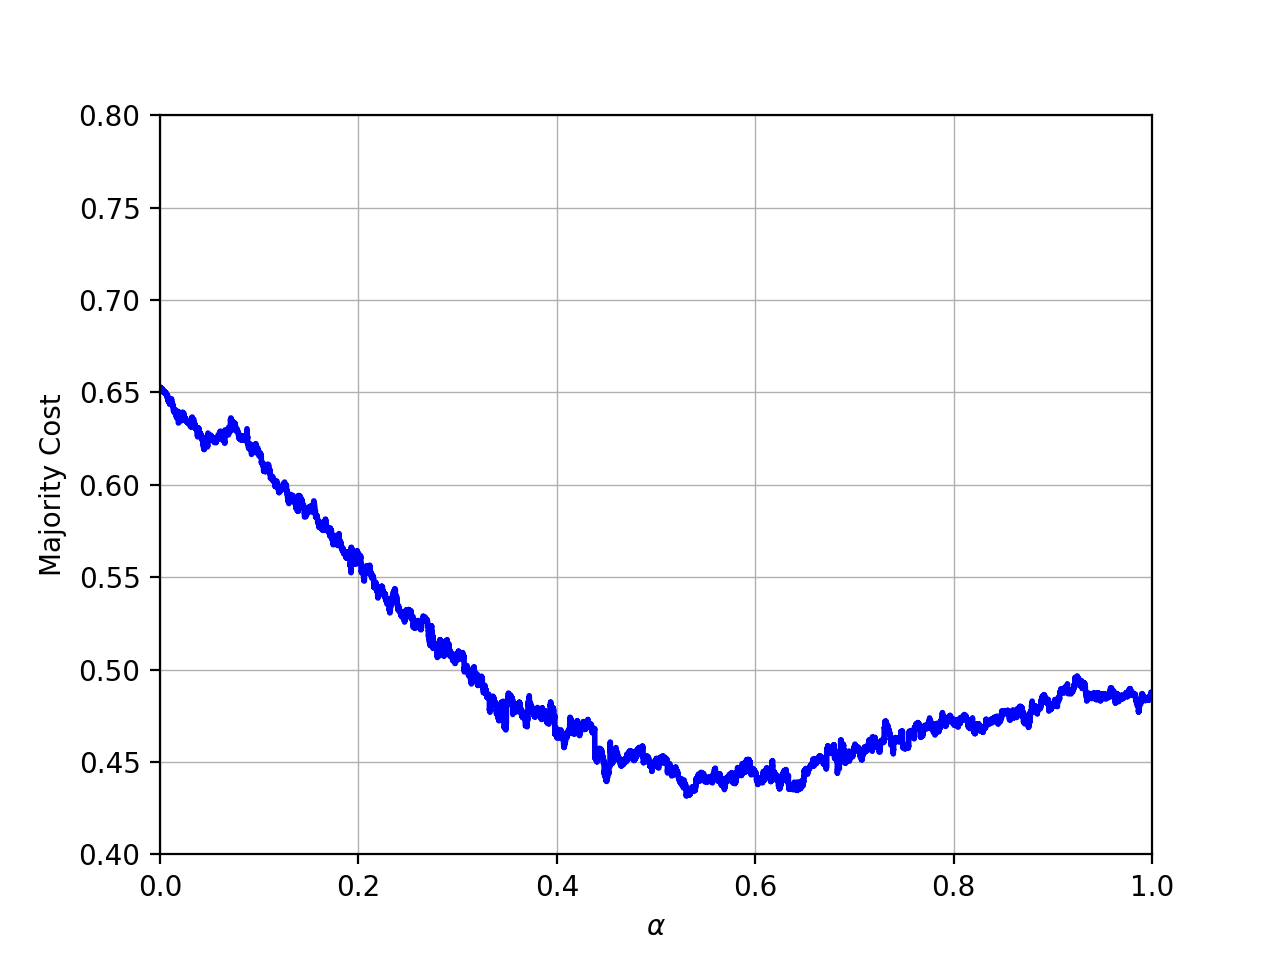
\includegraphics[width=\linewidth]{plots/mnist-ac-5}
\end{minipage}
\caption{Over the first six batches of the MNIST data, interpolating between average and complete linkage shows quite different curves.}
\label{fig:mnist1000acbatch}
\end{figure}

\begin{table}[h]
    \centering
    \begin{tabular}{|l | l l l l l l |}
    \hline
    Strategy & Batch 0 & Batch 1 & Batch 2 & Batch 3 & Batch 4 & Batch 5\\ \hline
    Average Linkage & 0.664952 & 0.672583 & 0.623325 & 0.679929 & 0.657857 & 0.652774\\
    Complete Linkage & 0.490468 & 0.461063 & 0.479825 & 0.475329 & 0.463321 & 0.487111\\
    $\alpha_{opt}$ & 0.7869 & 0.7124 & 0.634 & 0.807697 & 0.536073 & 0.5305\\
    $cost_{opt}$ & 0.458167 & 0.406563 & 0.440964 & 0.451063 & 0.429849 & 0.431631\\
    $\Delta cost$ & 3.2301\% & 5.45\% & 3.8861\% & 2.4266\% & 3.3472\% & 5.548\%\\\hline
    \end{tabular}
    \caption{$\alpha$-linkage reduces the cost of the MNIST dataset by up to $\Delta_{max} cost = 5.548\%$ when interpolating between average and complete linkage.}
    \label{table:mnist1000acbatch}
\end{table}

\begin{figure}[h]
\centering
\begin{minipage}{.45\textwidth}
  \centering
  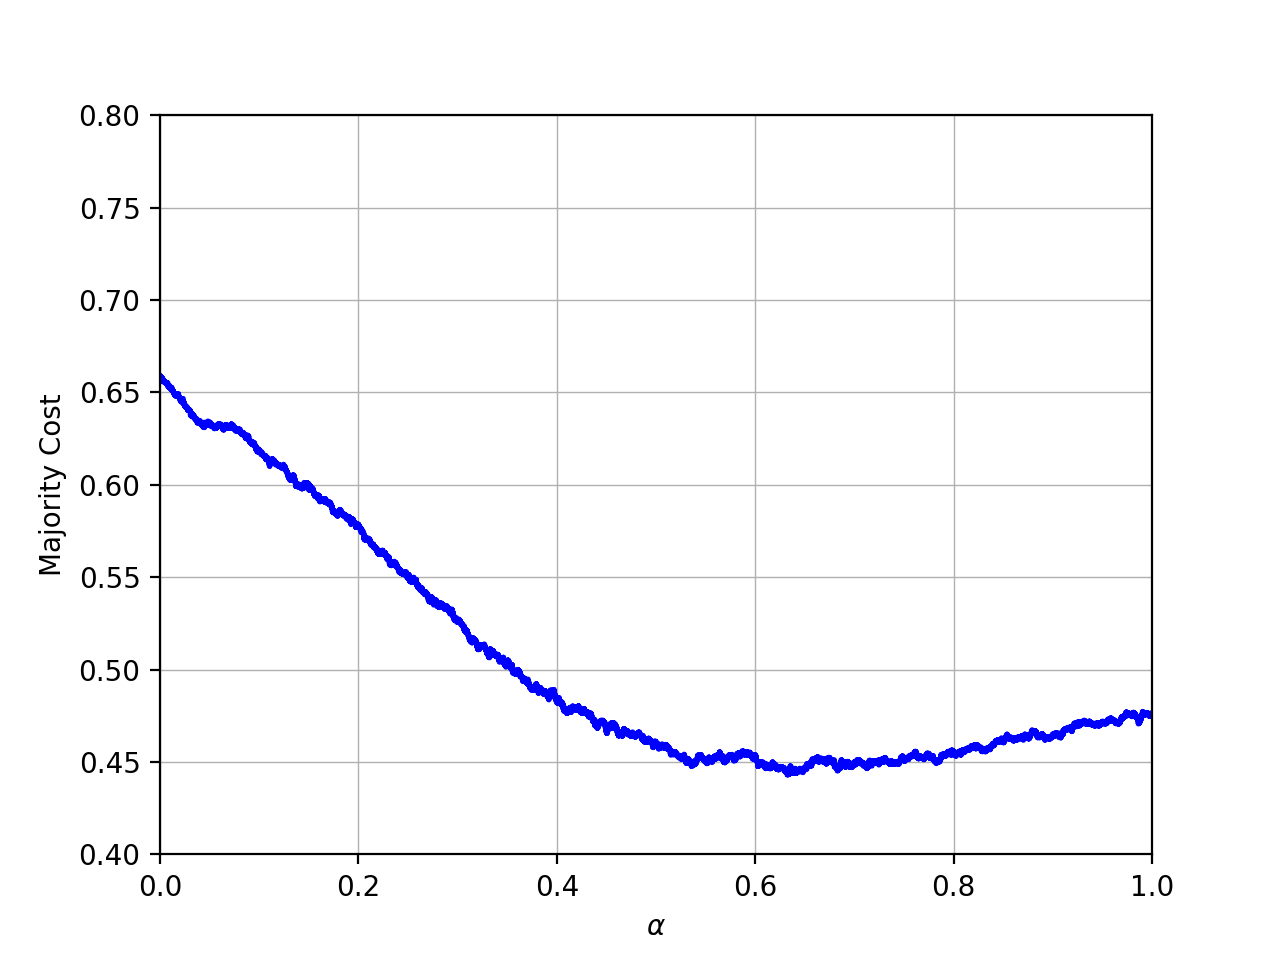
\includegraphics[width=\linewidth]{plots/mnist-ac-averaged}
\end{minipage}
\begin{minipage}{.45\textwidth}
  \centering
  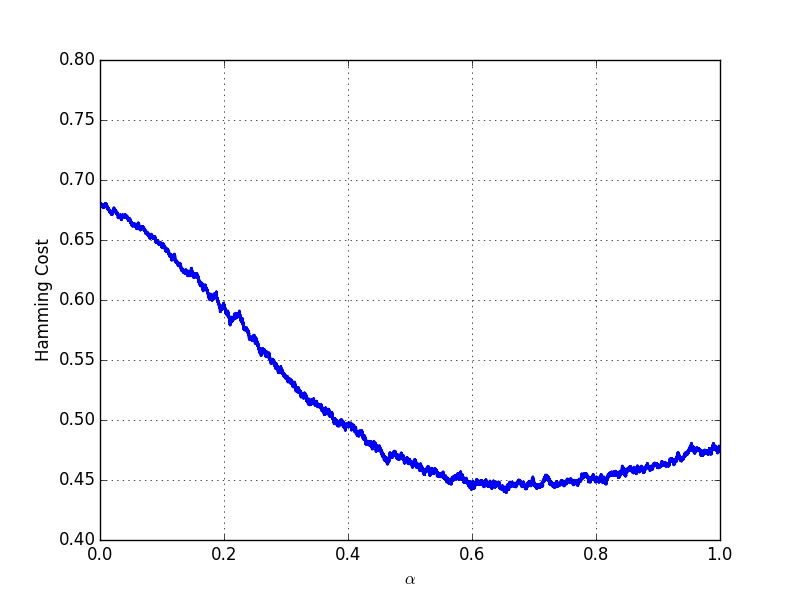
\includegraphics[width=\linewidth]{plots/mnist-ac-random}
\end{minipage}
\begin{minipage}{.45\textwidth}
  \centering
  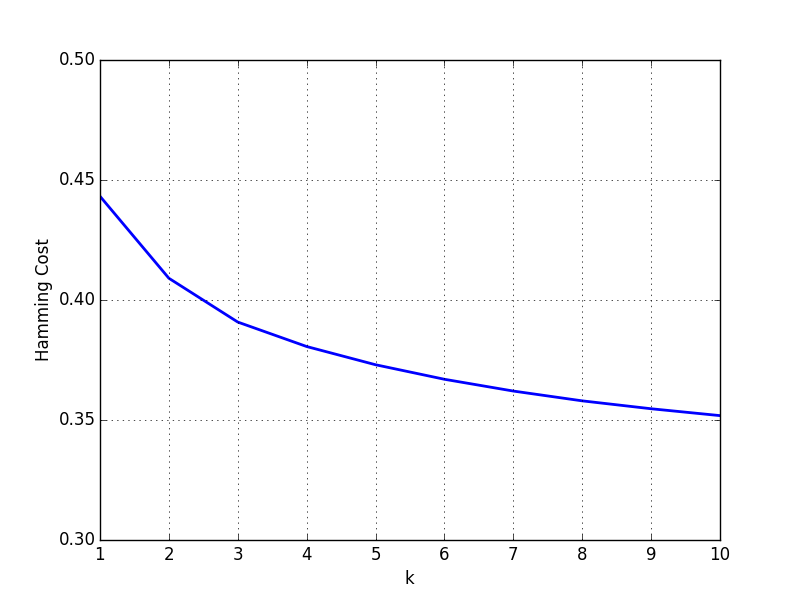
\includegraphics[width=\linewidth]{plots/mnist-ac-top-10}
\end{minipage}
\begin{minipage}{.45\textwidth}
  \centering
  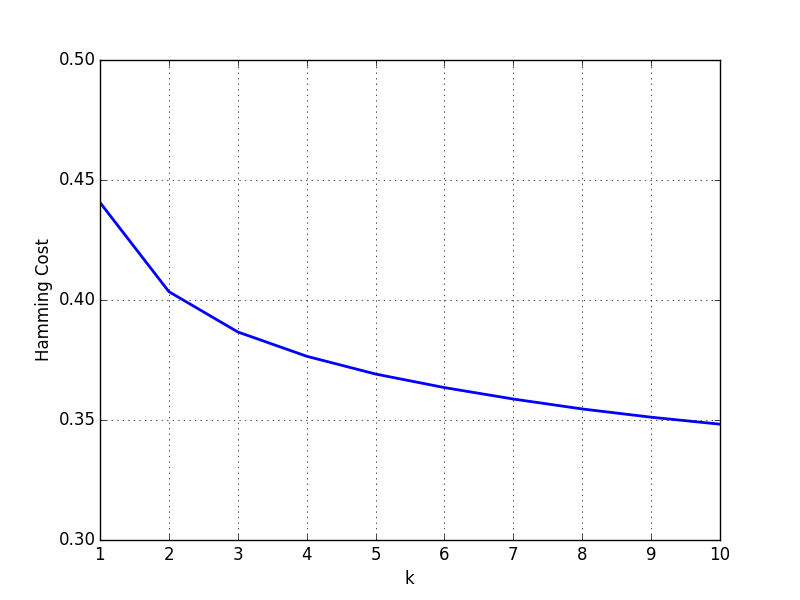
\includegraphics[width=\linewidth]{plots/mnist-ac-random-top-10}
\end{minipage}
\caption{Comparing the batch and the random experients for the MNIST data when interpolating between average and complete linkage leads to similar curves.}
\label{fig:mnistacavg}
\end{figure}

Figure \ref{fig:mnistacavg} shows the comparison between the batch (left) and the random experiments (right). In general, we obtain similarly looking curves, but elaborate the results further in table \ref{table:mnistacavg}.

\begin{table}[h]
    \centering
    \begin{tabular}{|l | l | l |}
    \hline
    Strategy & Hamming Cost (Batch) & Hamming Cost (Random)\\ \hline
    Average Linkage & 0.65857 & 0.679936\\
    Complete Linkage & 0.476187 & 0.476328\\
    $\alpha_{opt}$ & 0.633 & 0.656\\
    $cost_{opt}$ & 0.44314 & 0.439632\\
    $\Delta cost$ & 3.3047\% & 3.6696\%\\\hline
    \end{tabular}
    \caption{}
    \label{table:mnistacavg}
\end{table}

Summarizing, we also obtained very positive results for $d_{AC}$, however the results were not as stable as for $d_{SC}$. In our experiments, we notice that $d_{SC}$ results in more discontinuities (factor $\approx 3$) than $d_{AC}$. This may be because the distance $d(\alpha)$ is wider spread for $d_{SC}$, i.e. $|d_{SC}(\alpha = 1) - d_{SC}(\alpha = 0)| > |d_{AC}(\alpha = 1) - d_{AC}(\alpha = 0)|$. However $d_{AC}$ is dependant on more points, so it may be an indicator for this observation, but not a proof. Figure \ref{fig:mnistactop10} also shows that parameter advising is using with a small value $k$ already and reduces the costs for $k = 3$ by $\approx 5\%$ in addition.

\paragraph{Learning MNIST features.} Differently to just using the raw pixel features, we here apply preprocessing techniques with the intention to generate more accurate clusterings. As in section \ref{sec:imagefeatures} described, we use a Convolutional Neural Network to learn a more robust and lower-dimensional feature representation. Therefore, we use the in appendix \ref{sec:cnnarchitecture} described architecture, train the network with all data and then extract the features by cutting off the last three layers of the network. This then results in a learned 128-dimensional representation for each image.

\begin{figure}[h]
\centering
\begin{minipage}{.45\textwidth}
  \centering
  \subcaptionbox{By evaluating all 252 combinations of five different labels, the average error goes down to $2.6\%$ that makes an improvement of $7.4\%$ compared to complete linkage.}
  {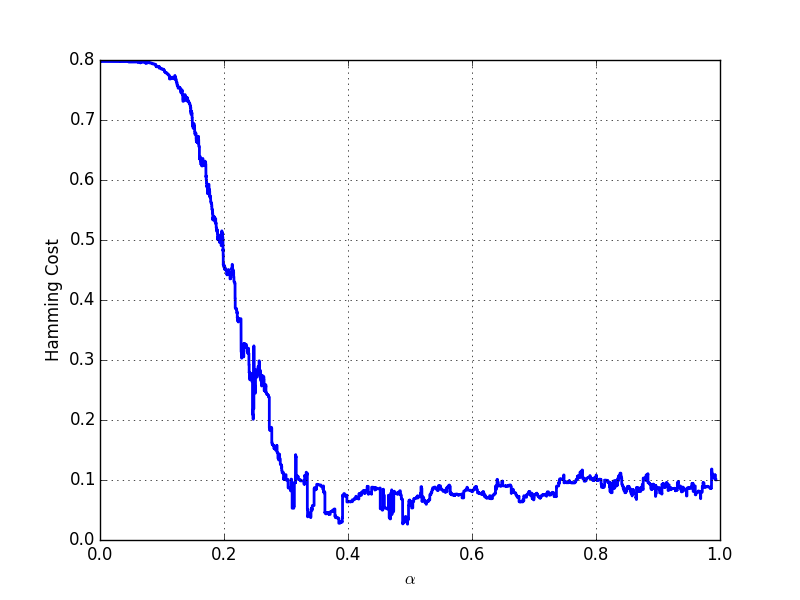
\includegraphics[width=\linewidth]{plots/mnist-cnn-avg}}
\end{minipage}\quad
\begin{minipage}{.45\textwidth}
  \centering
  \subcaptionbox{Evaluating 512 random sets of labels and points gives an eror of $7.1\%$ that is an improvement of $1.9\%$ compared to complete linkage.}
  {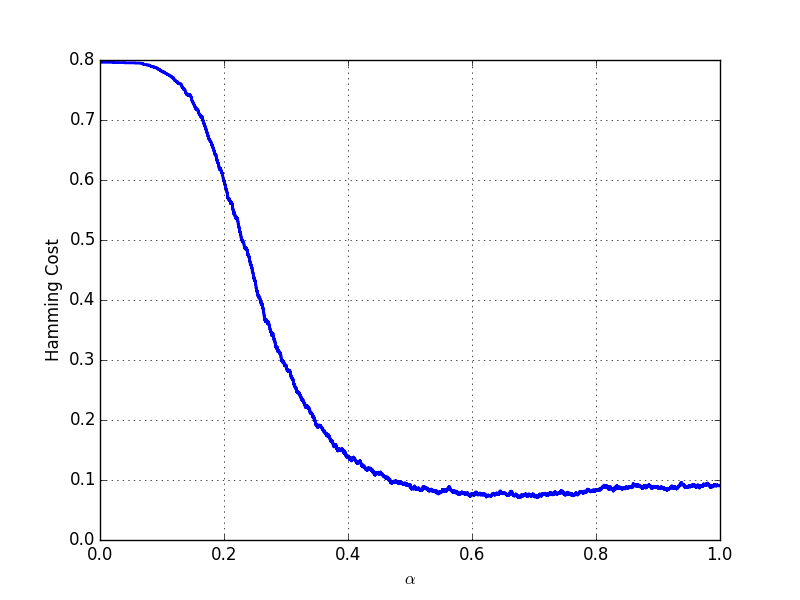
\includegraphics[width=\linewidth]{plots/mnist-cnn-random}}
\end{minipage}
\begin{minipage}{.45\textwidth}
  \centering
  \subcaptionbox{Considerung more than one optimal value to evaluate the experiments results in lower costs, e.g. using two values $\alpha_{opt}$ cuts the cost by $50\%$ and using three values results in a cost below $1\%$.}
  {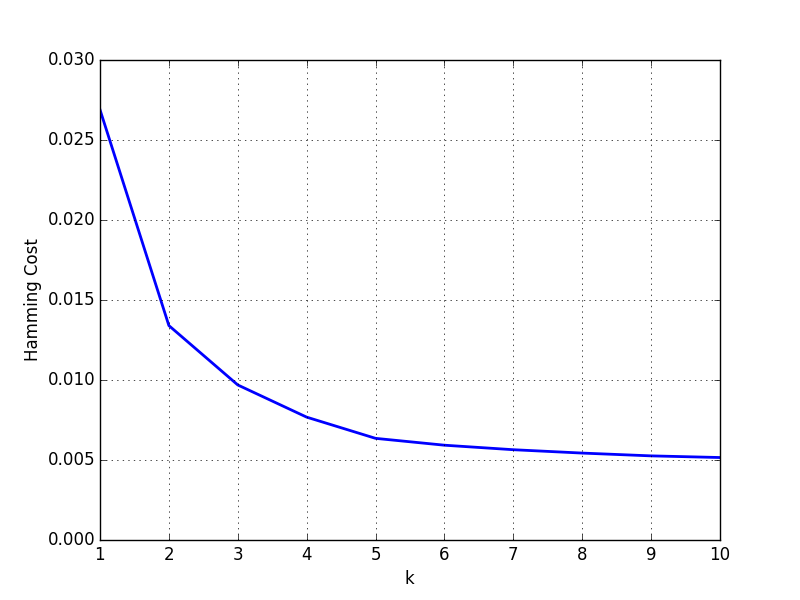
\includegraphics[width=\linewidth]{plots/mnist-cnn-sc-top-10}}
\end{minipage}\quad
\begin{minipage}{.45\textwidth}
  \centering
  \subcaptionbox{On random sets of labels and randomly selected points, taking more than one optimal value $\alpha_{opt}$ also gives major improvements. With three values the cost goes down below $3\%$ that is less than a half of the original optimum.}
  {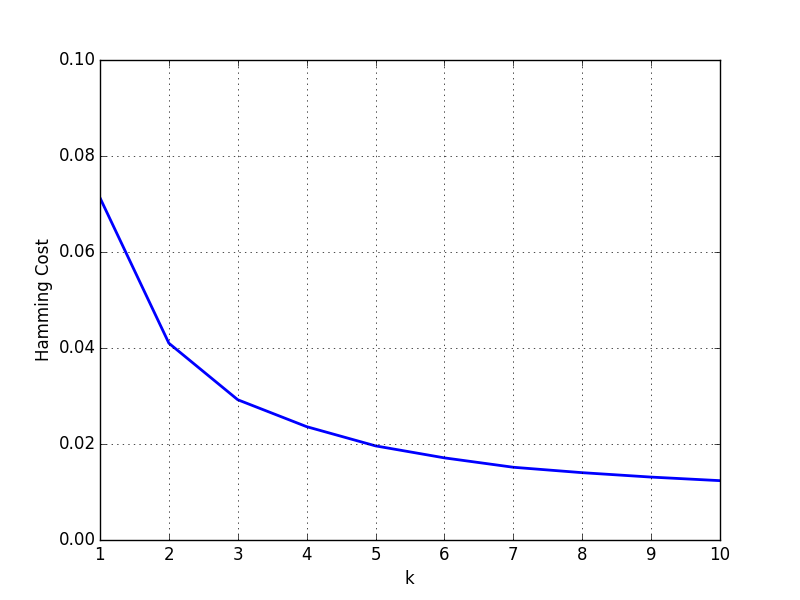
\includegraphics[width=\linewidth]{plots/mnist-cnn-sc-random-top-10}}
\end{minipage}
\caption{By learning feature representations with a Convolutional Neural Network, we can reduce the overall error a lot compared to clustering raw pixel images.}
\label{fig:mnist1000cnn}
\end{figure}

Figure \ref{fig:mnist1000cnn} shows that single linkage still performs poorly, however the error for both complete linkage and the interval in between are much lower. Also, we note that the improvement using $\alpha$-linkage is large over both settings. However, a Convolutional Neural Network aims at recognizing the characters, so training on all images might be the sole cause of our improvements. Thus, it is more relevant for our experiments to either train the network on a subset of the data or to train the network on a different task in order to transfer the knowledge to unseen data or to a different task.

\paragraph{Learning Subsets of the MNIST Data.} As our goal is also to cluster unseen data, we evaluated another setup, where a CNN was trained on a subset of the dataset. In a first attempt, we trained it on the labels $\{0,1,2,3,4\}$ that are represented with 30,000 of the 60,000 points in the dataset. Figure \ref{fig:mnist1000cnnsub} shows that clustering unseen points (i.e. the CNN did not use these points for training) still results in a lower error than using the raw pixel features where combining seen and unseen points leads to results that are comparable to clusterings with features extracted from a neural network that was trained with all digits. In average, complete linkage resulted in an error of $22.1\%$. The cost for $\alpha_{opt} = 0.67$ is $20.7\%$ and makes an improvement of $1.4\%$. Interesting especially in this setting are the different results of seen and unseen data. In machine learning, the task of applying knowledge to unseen data is commonly known as zero-shot learning. While the error was $0.2\%$ for large parts of the seen data (i.e. clustering the digits $\{0,1,2,3,4\}$), the optimal cost for the unseen data (i.e. clustering the digits $\{5,6,7,8,9\}$) was $24.7\%$ for $\alpha_{opt} = 0.76$. \todo[inline]{plot and discuss randomized experiments}

\begin{figure}[h]
\centering
\begin{minipage}{.3\textwidth}
  \centering
  \subcaptionbox{The learned characters (i.e. labels $\{0,1,2,3,4\}$) can be clustered very well. Similar to training on all labels, the error goes down close to $0\%$.}
  {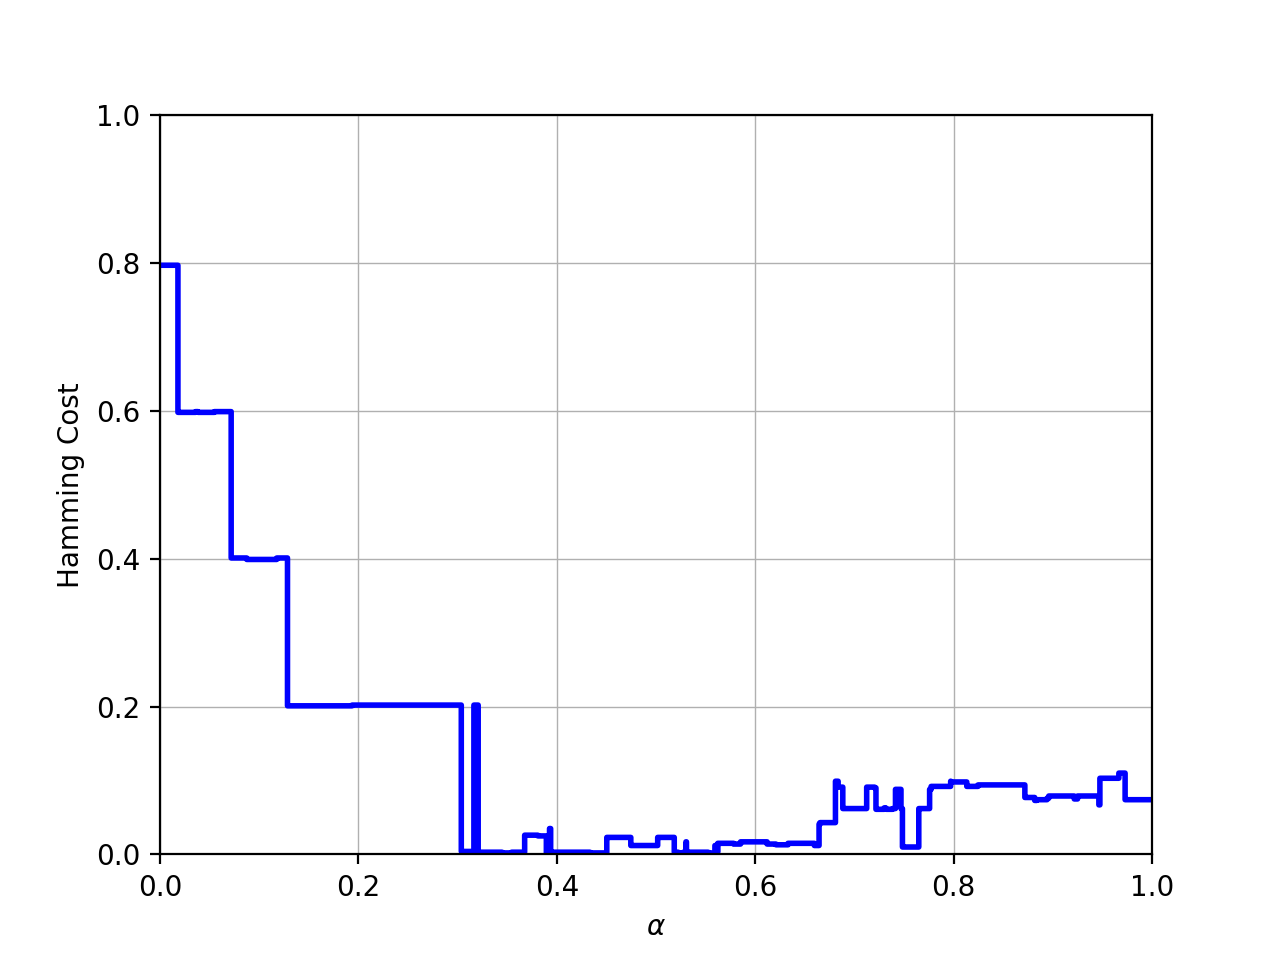
\includegraphics[width=\linewidth]{plots/mnist-cnn-sub-01234}}
\end{minipage}\quad
\begin{minipage}{.3\textwidth}
  \centering
  \subcaptionbox{Combining three trained ($0,2,4$) with two untrained digits ($6,8$) still leads to an optimal error of $2.1\%$ that is $10\%$ below complete linkage.}
  {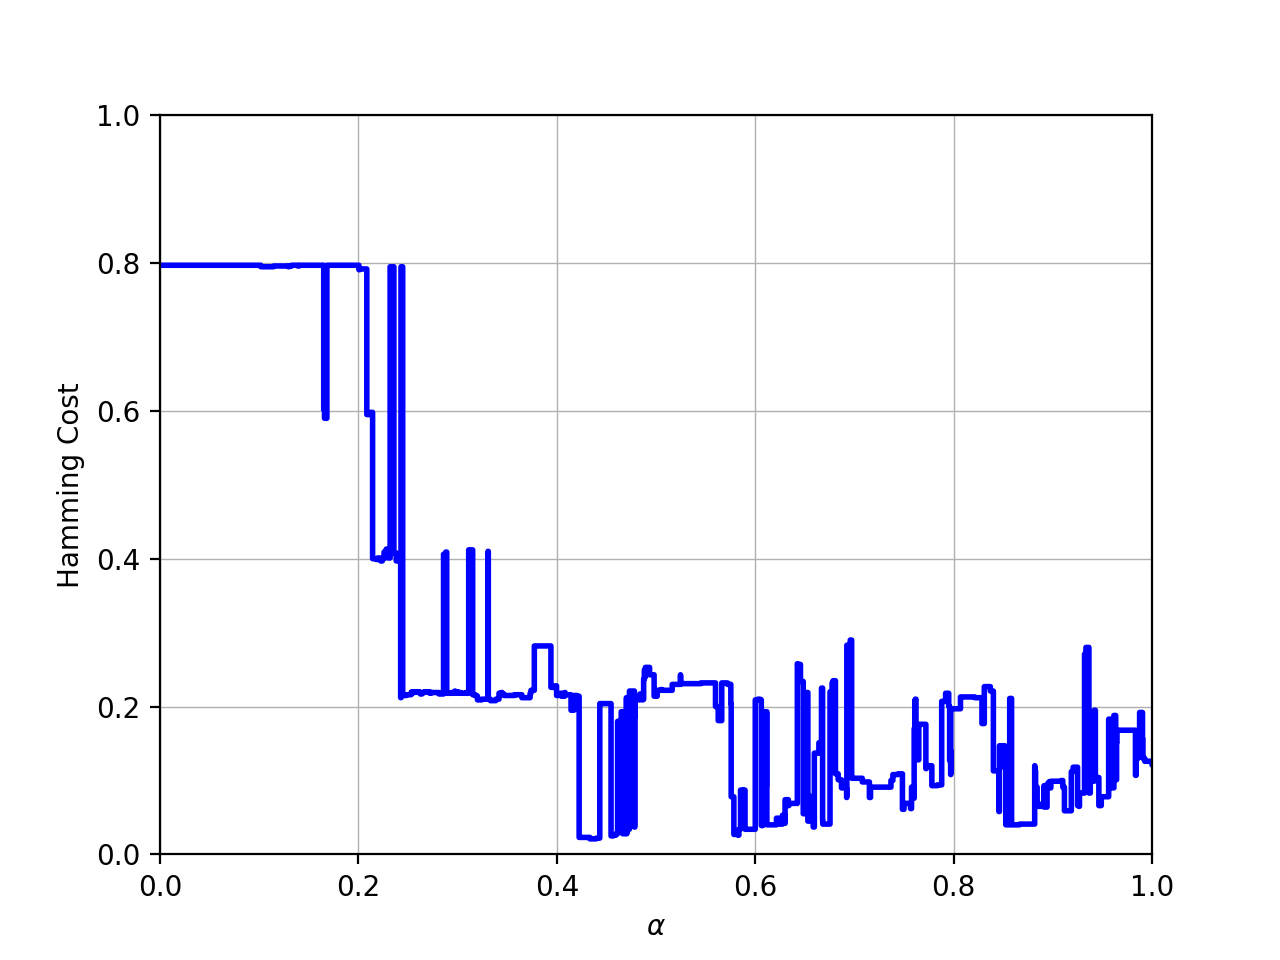
\includegraphics[width=\linewidth]{plots/mnist-cnn-sub-02468}}
\end{minipage}\quad
\begin{minipage}{.3\textwidth}
  \centering
  \subcaptionbox{Clustering three untrained ($5,7,9$) with two trained digits ($1,3$) already leads to larger errors of $15.1\%$.}
  {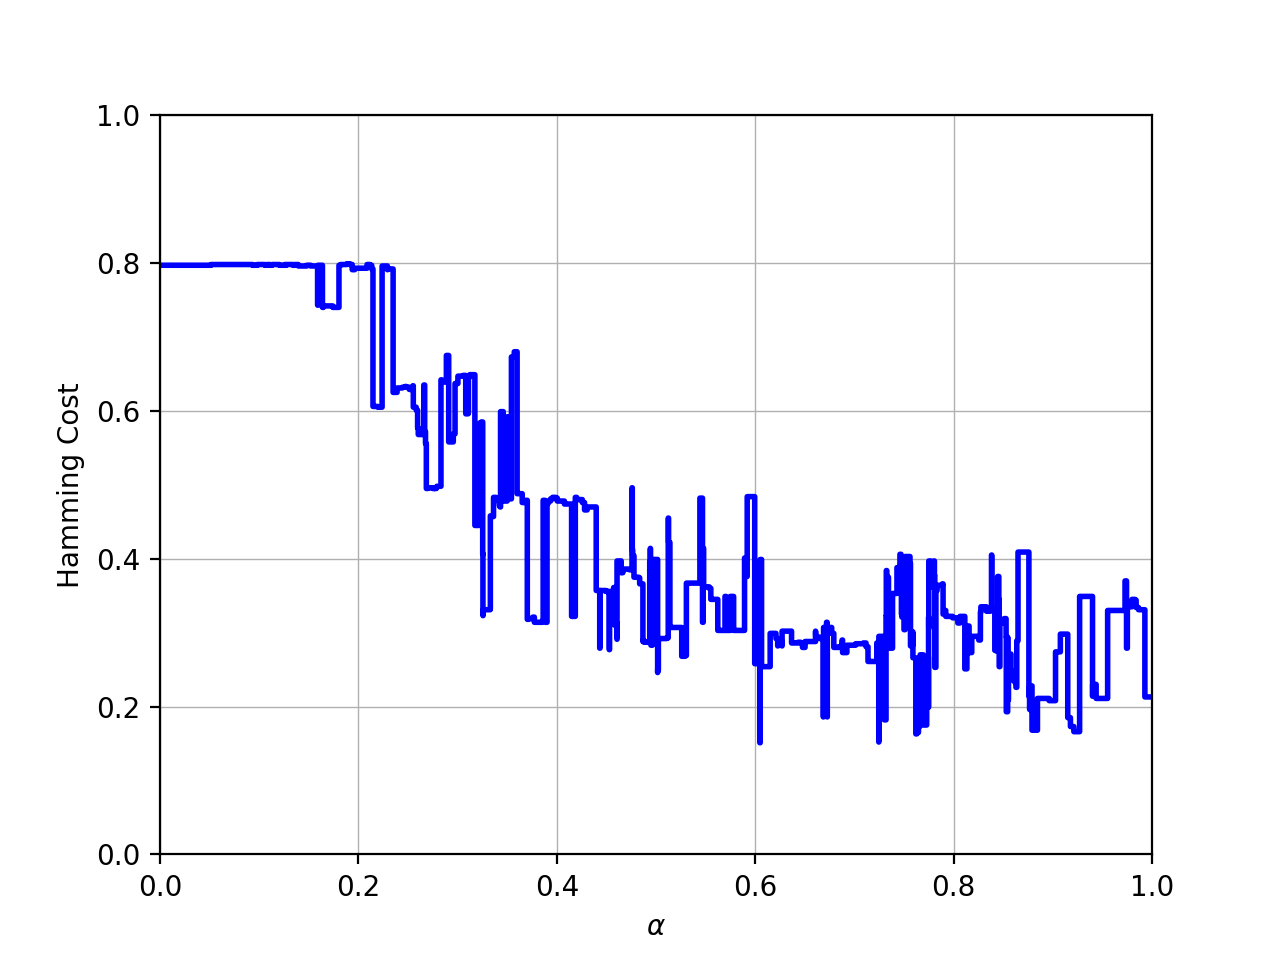
\includegraphics[width=\linewidth]{plots/mnist-cnn-sub-13579}}
\end{minipage}
\begin{minipage}{.3\textwidth}
  \centering
  \subcaptionbox{Even by clustering only untrained characters, the error goes down to $37\%$ that is a major improvement compared to clustering the raw pixel features that resulted in an optimal cost of $44\%$.}
  {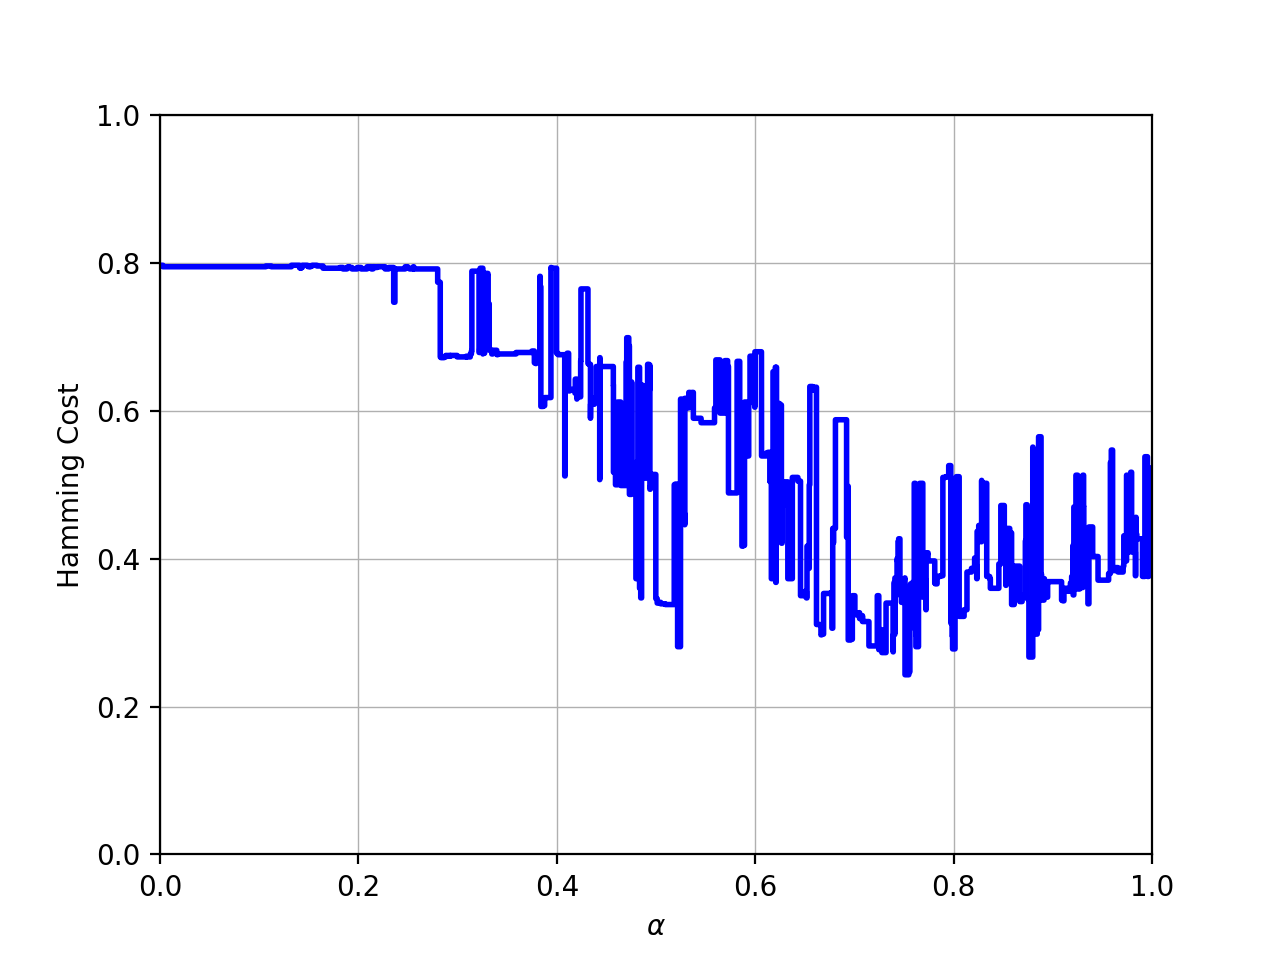
\includegraphics[width=\linewidth]{plots/mnist-cnn-sub-56789}}
\end{minipage}\quad
\begin{minipage}{.3\textwidth}
  \centering
  \subcaptionbox{Averaged over all 252 instances, the error for $\alpha_{opt} = 0.67$ is $20.7\%$ and an improvement of $1.4\%$ compared to complete linkage and $23\%$ compared to the raw pixel features.}
  {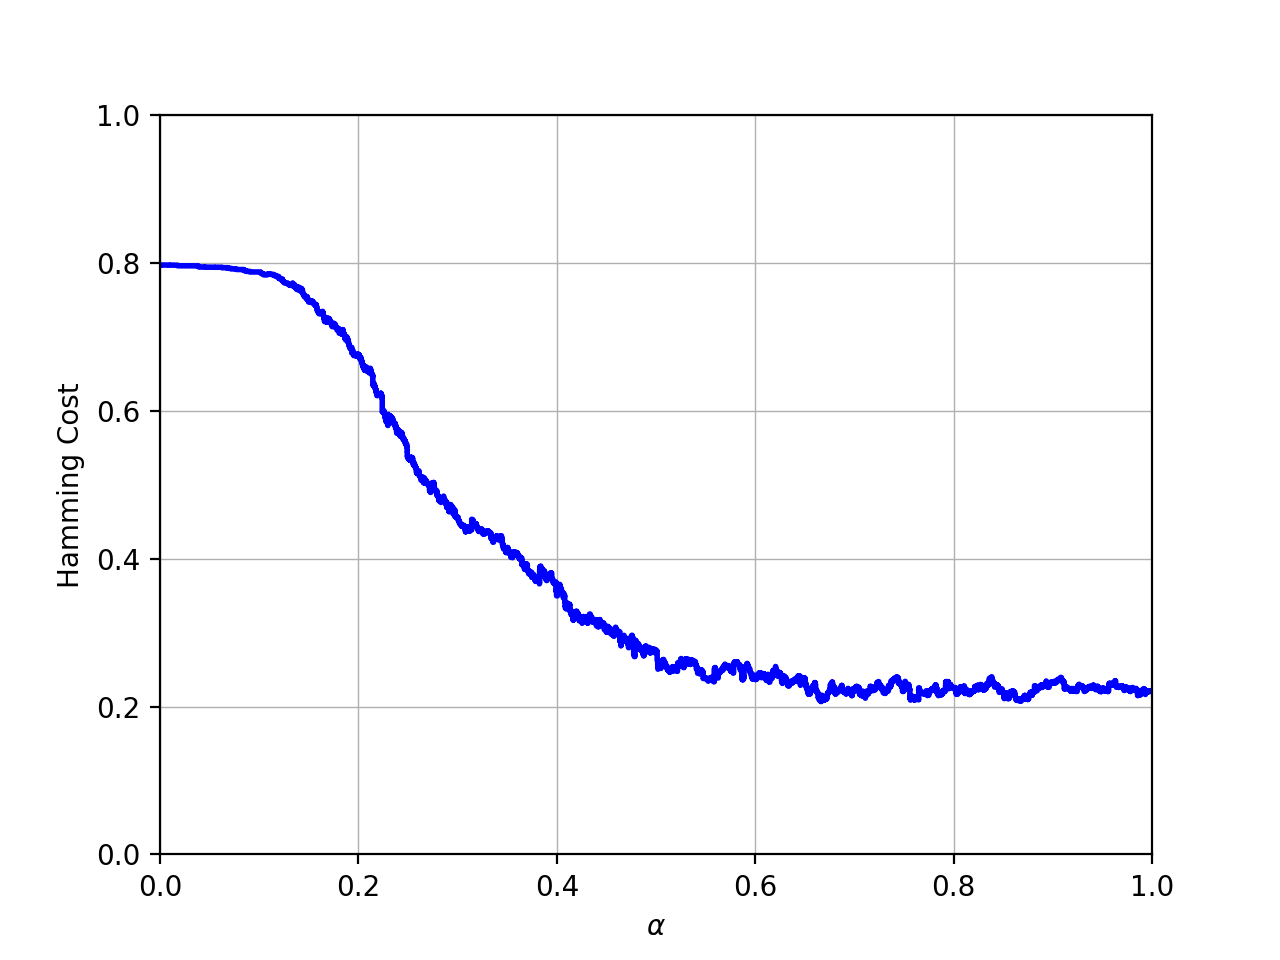
\includegraphics[width=\linewidth]{plots/mnist-cnn-sub-sc}}
\end{minipage}\quad
\begin{minipage}{.3\textwidth}
  \centering
  \subcaptionbox{Parameter advising results in major improvements for this setting. Using three values $\alpha^* \in \{0.86, 0.67, 0.99\}$ reduces the error by additional $5.3\%$ to $15.5\%$.} 
  {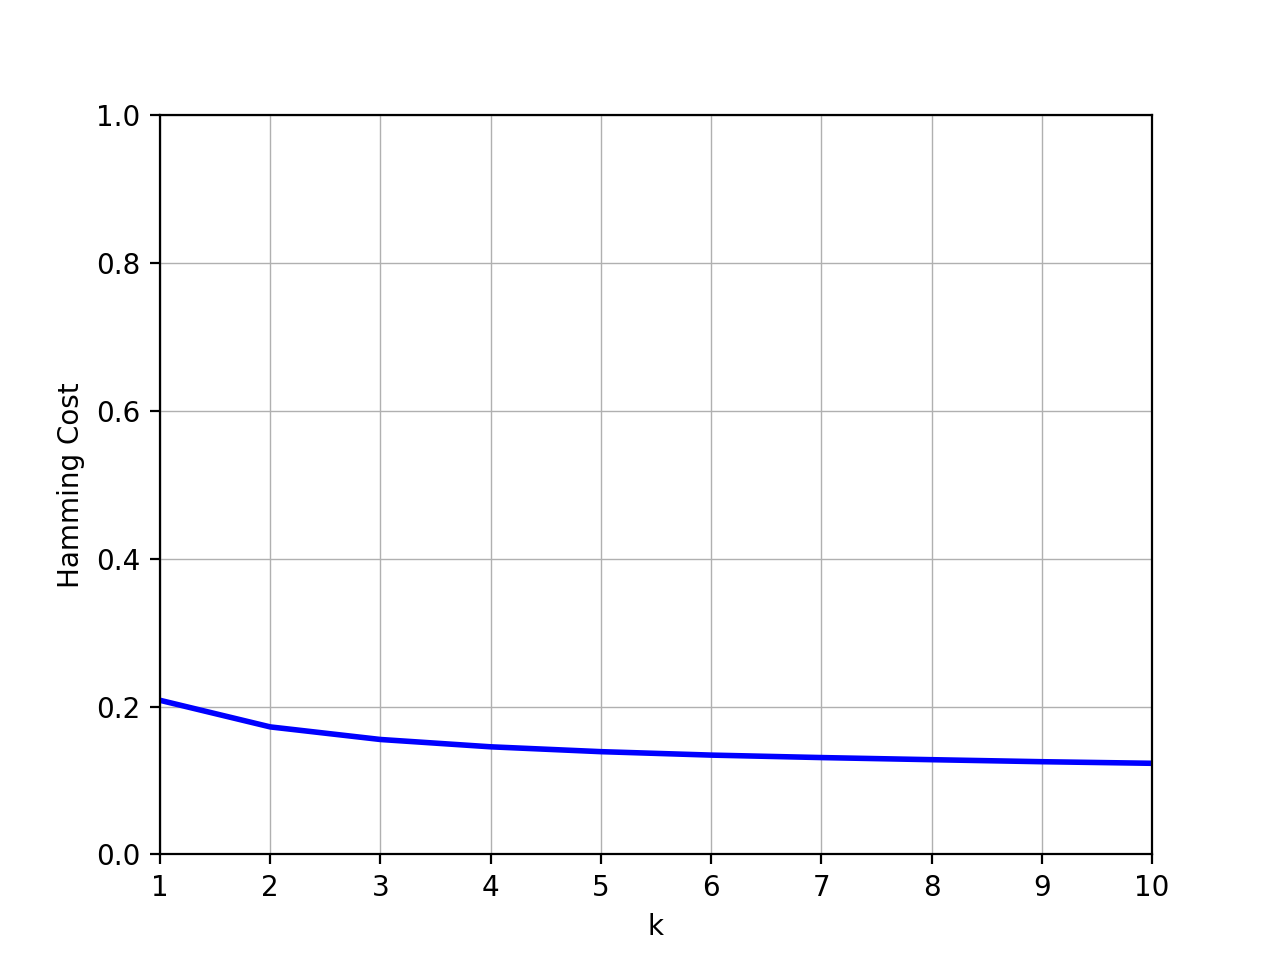
\includegraphics[width=\linewidth]{plots/mnist-cnn-sub-sc-top10}}
\end{minipage}
\caption{Learning features depending on a subset of the represented digits leads to different results. While applying the learned digits still leads to almost perfect clusterings, clustering the unlearned digits leads to worse results that still are much better than applying the raw pixel features.}
\label{fig:mnist1000cnnsub}
\end{figure}

\paragraph{Learning Even and Odd Numbers.} Beside training a neural network on recognizing all digits separately, another learning task to generate feature representations that we used is to learn if an image shows an even or an odd digit. In this setting, we trained the CNN on all images and extracted the feature vectors from the sixth layer. The used network had the same architecture as the one used in the earlier experiments with the only difference of two neurons in the output layer. Figure \ref{fig:mnist_cnn_even_odd} shows that with features trained on a different learning task we still can improve the overall clustering. Complete linkage resulted in a cost of $28.1\%$ for the first data batch, where the optimal alpha $\alpha_{opt} = 0.74$ led to $23.6\%$, an improvement of 4.5\%. The results are only slidely worse than the ones of a network trained to distinguish the digits $\{0,1,2,3,4\}$. Parameter adivising lowers the cost another $5.2\%$ for $n = 3$ values $\alpha^* \in \{0.74, 0.65, 0.76\}$. \todo[inline]{randomized experiments}

\begin{figure}[h]
\centering
\begin{minipage}{.45\textwidth}
  \centering
  \subcaptionbox{Compared to complete linkage, we got an improvement of $4.5\%$ for $\alpha_{opt} = 0.74$.}
  {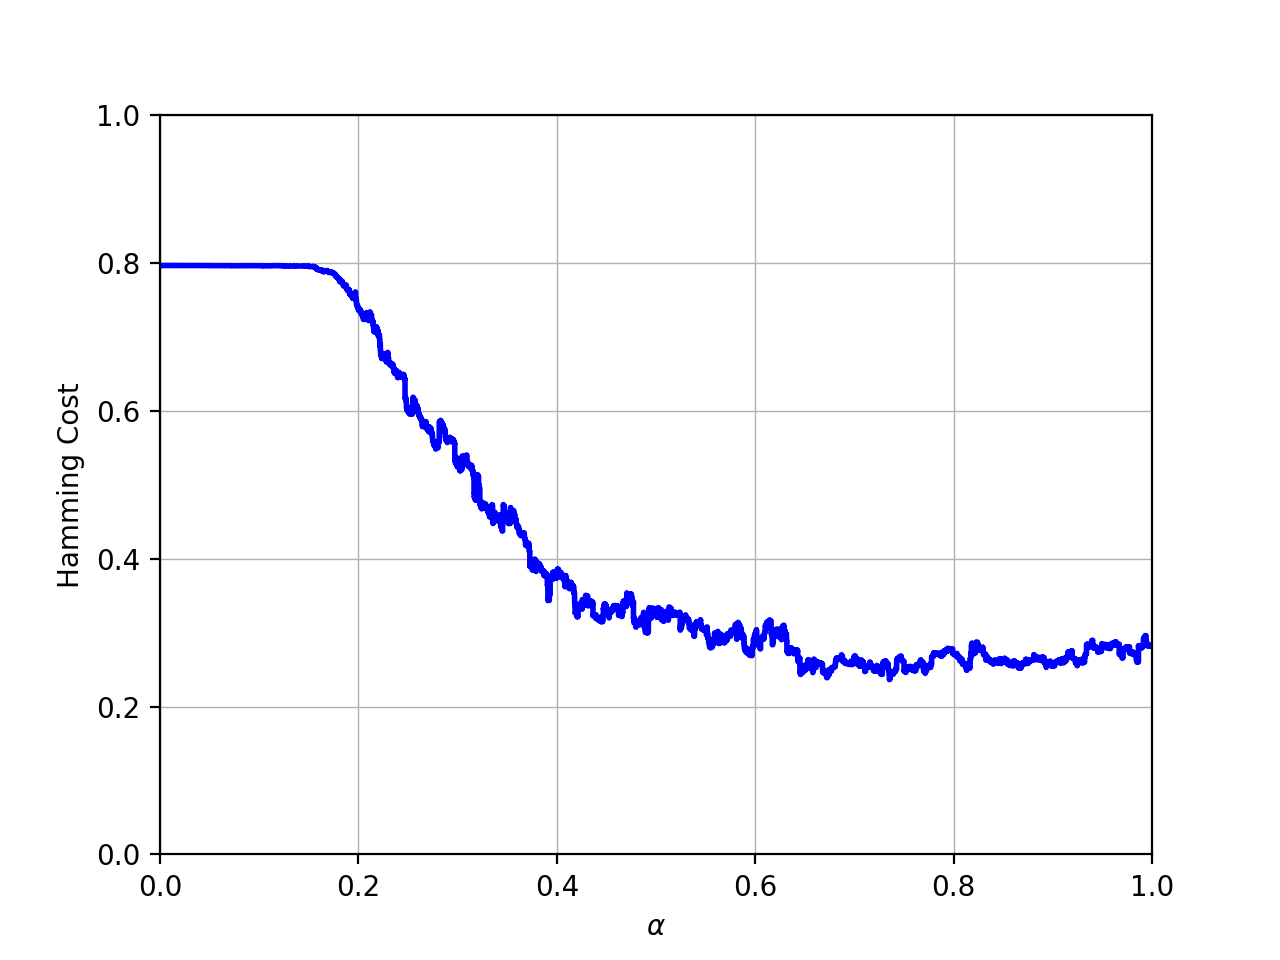
\includegraphics[width=\linewidth]{plots/mnist-cnn-even-odd-sc}}
\end{minipage}\quad
\begin{minipage}{.45\textwidth}
  \centering
  \subcaptionbox{Applying parameter advising shows significant improvements for small numbers of $k$.}
  {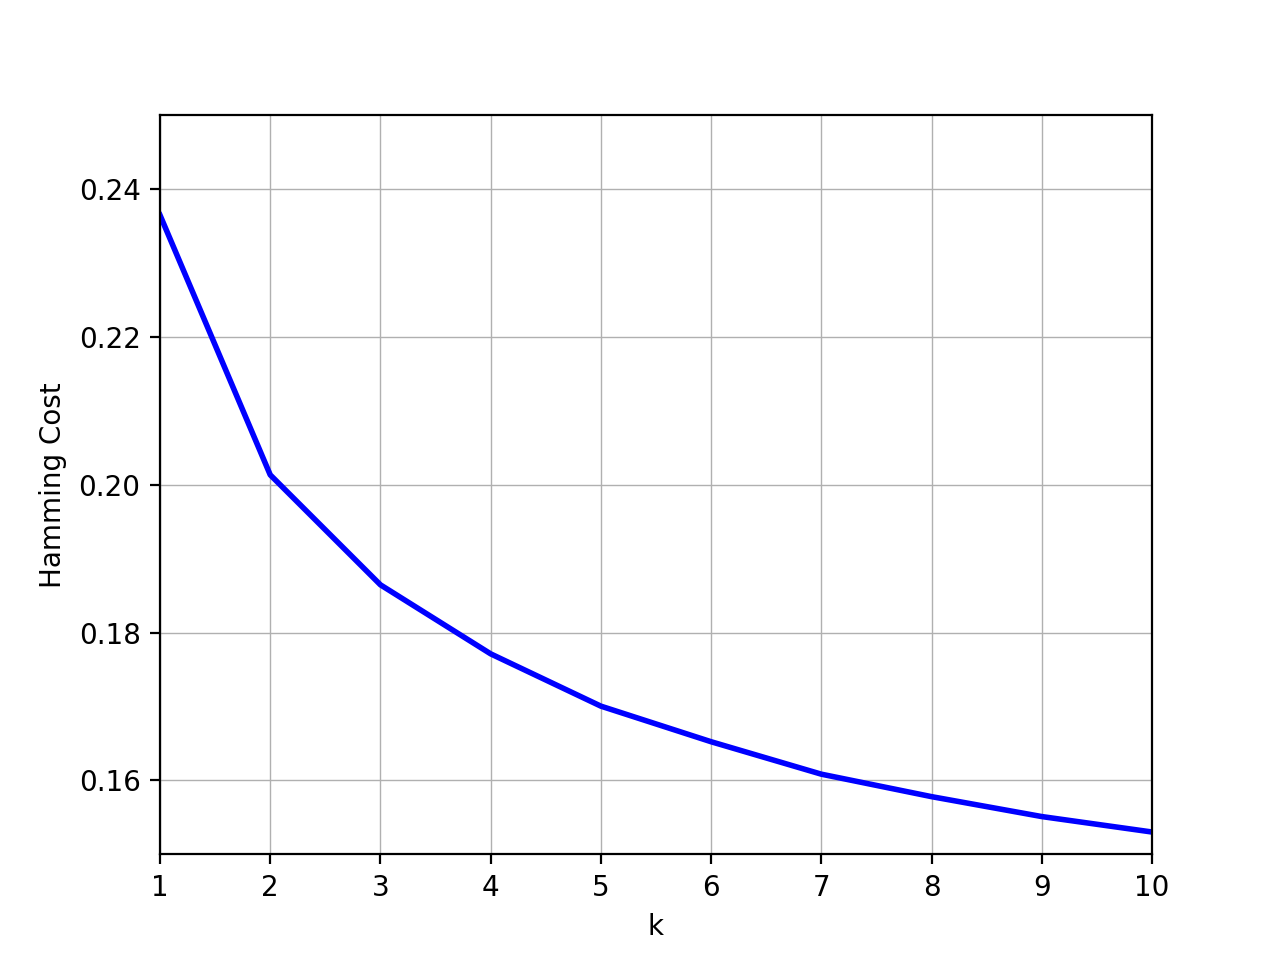
\includegraphics[width=\linewidth]{plots/mnist-cnn-even-odd-sc-top10}}
\end{minipage}
\begin{minipage}{.45\textwidth}
  \centering
  \subcaptionbox{.}
  {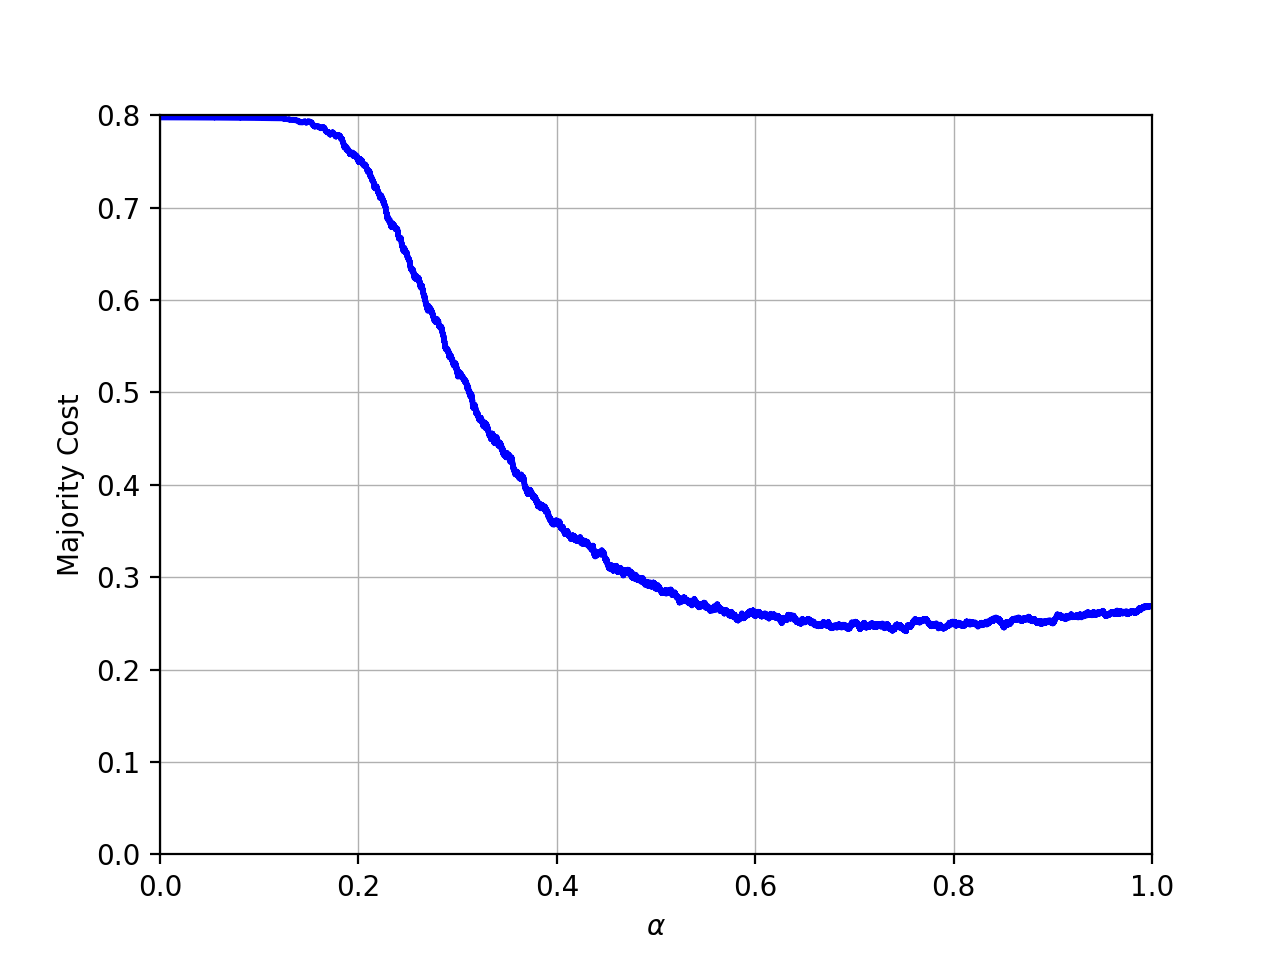
\includegraphics[width=\linewidth]{plots/mnist-cnn-even-odd-random-sc}}
\end{minipage}\quad
\begin{minipage}{.45\textwidth}
  \centering
  \subcaptionbox{.}
  {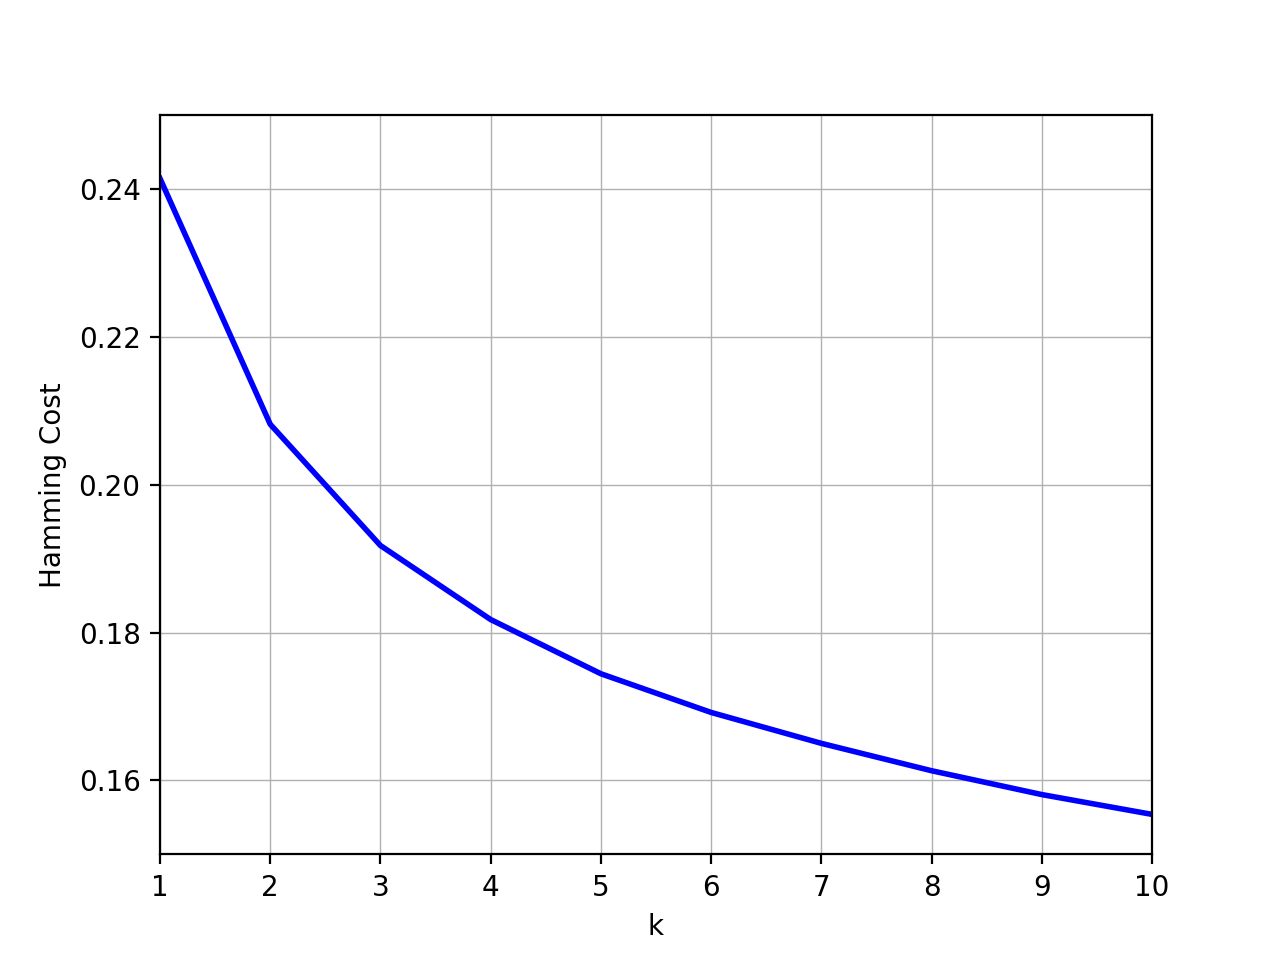
\includegraphics[width=\linewidth]{plots/mnist-cnn-even-odd-random-sc-top10}}
\end{minipage}
\caption{%
  %
  Clustering features extracted from a CNN that learned to distinguish even from odd numbers with all data led to an optimal cost of $23.6\%$ (a). Parameter advising allows us to minimize the cost ether further to $18.4\%$ for the values $\alpha^* \in \{0.74, 0.65, 0.76\}$ (b).}
  %
\label{fig:mnist_cnn_even_odd}
\end{figure}

\paragraph{Summarized MNIST Results.} Different experimental setups were discussed in this section. First, raw pixel features were used for clustering. Later on, features extracted from Convolutional Neural Networks were used. There, we trained a network on all digits and extracted the feature vectors from the 6th layer of the network that represents each image encoded in a 128-dimensional vector. We used the same representation coming from a network trained on a subset of the images. In addition, we extracted feature vectors from the 9216-dimensional 5th layer of the network that was trained on a subset of the characters. Figure \ref{fig:mnist_overview} gives an overview about the results of the different settings for both the 252 experiments evaluating all different combinations of five labels within the first data batch as well as the randomized experiments where we evaluated 512 experiments with radomized digits and points from the entire data. \todo{add table}

\begin{figure}[h]
\centering
\begin{minipage}{.45\textwidth}
  \centering
  \subcaptionbox{Evaluating the experiments of all combinations of five labels within the first batch shows strong discontinuities.}
  {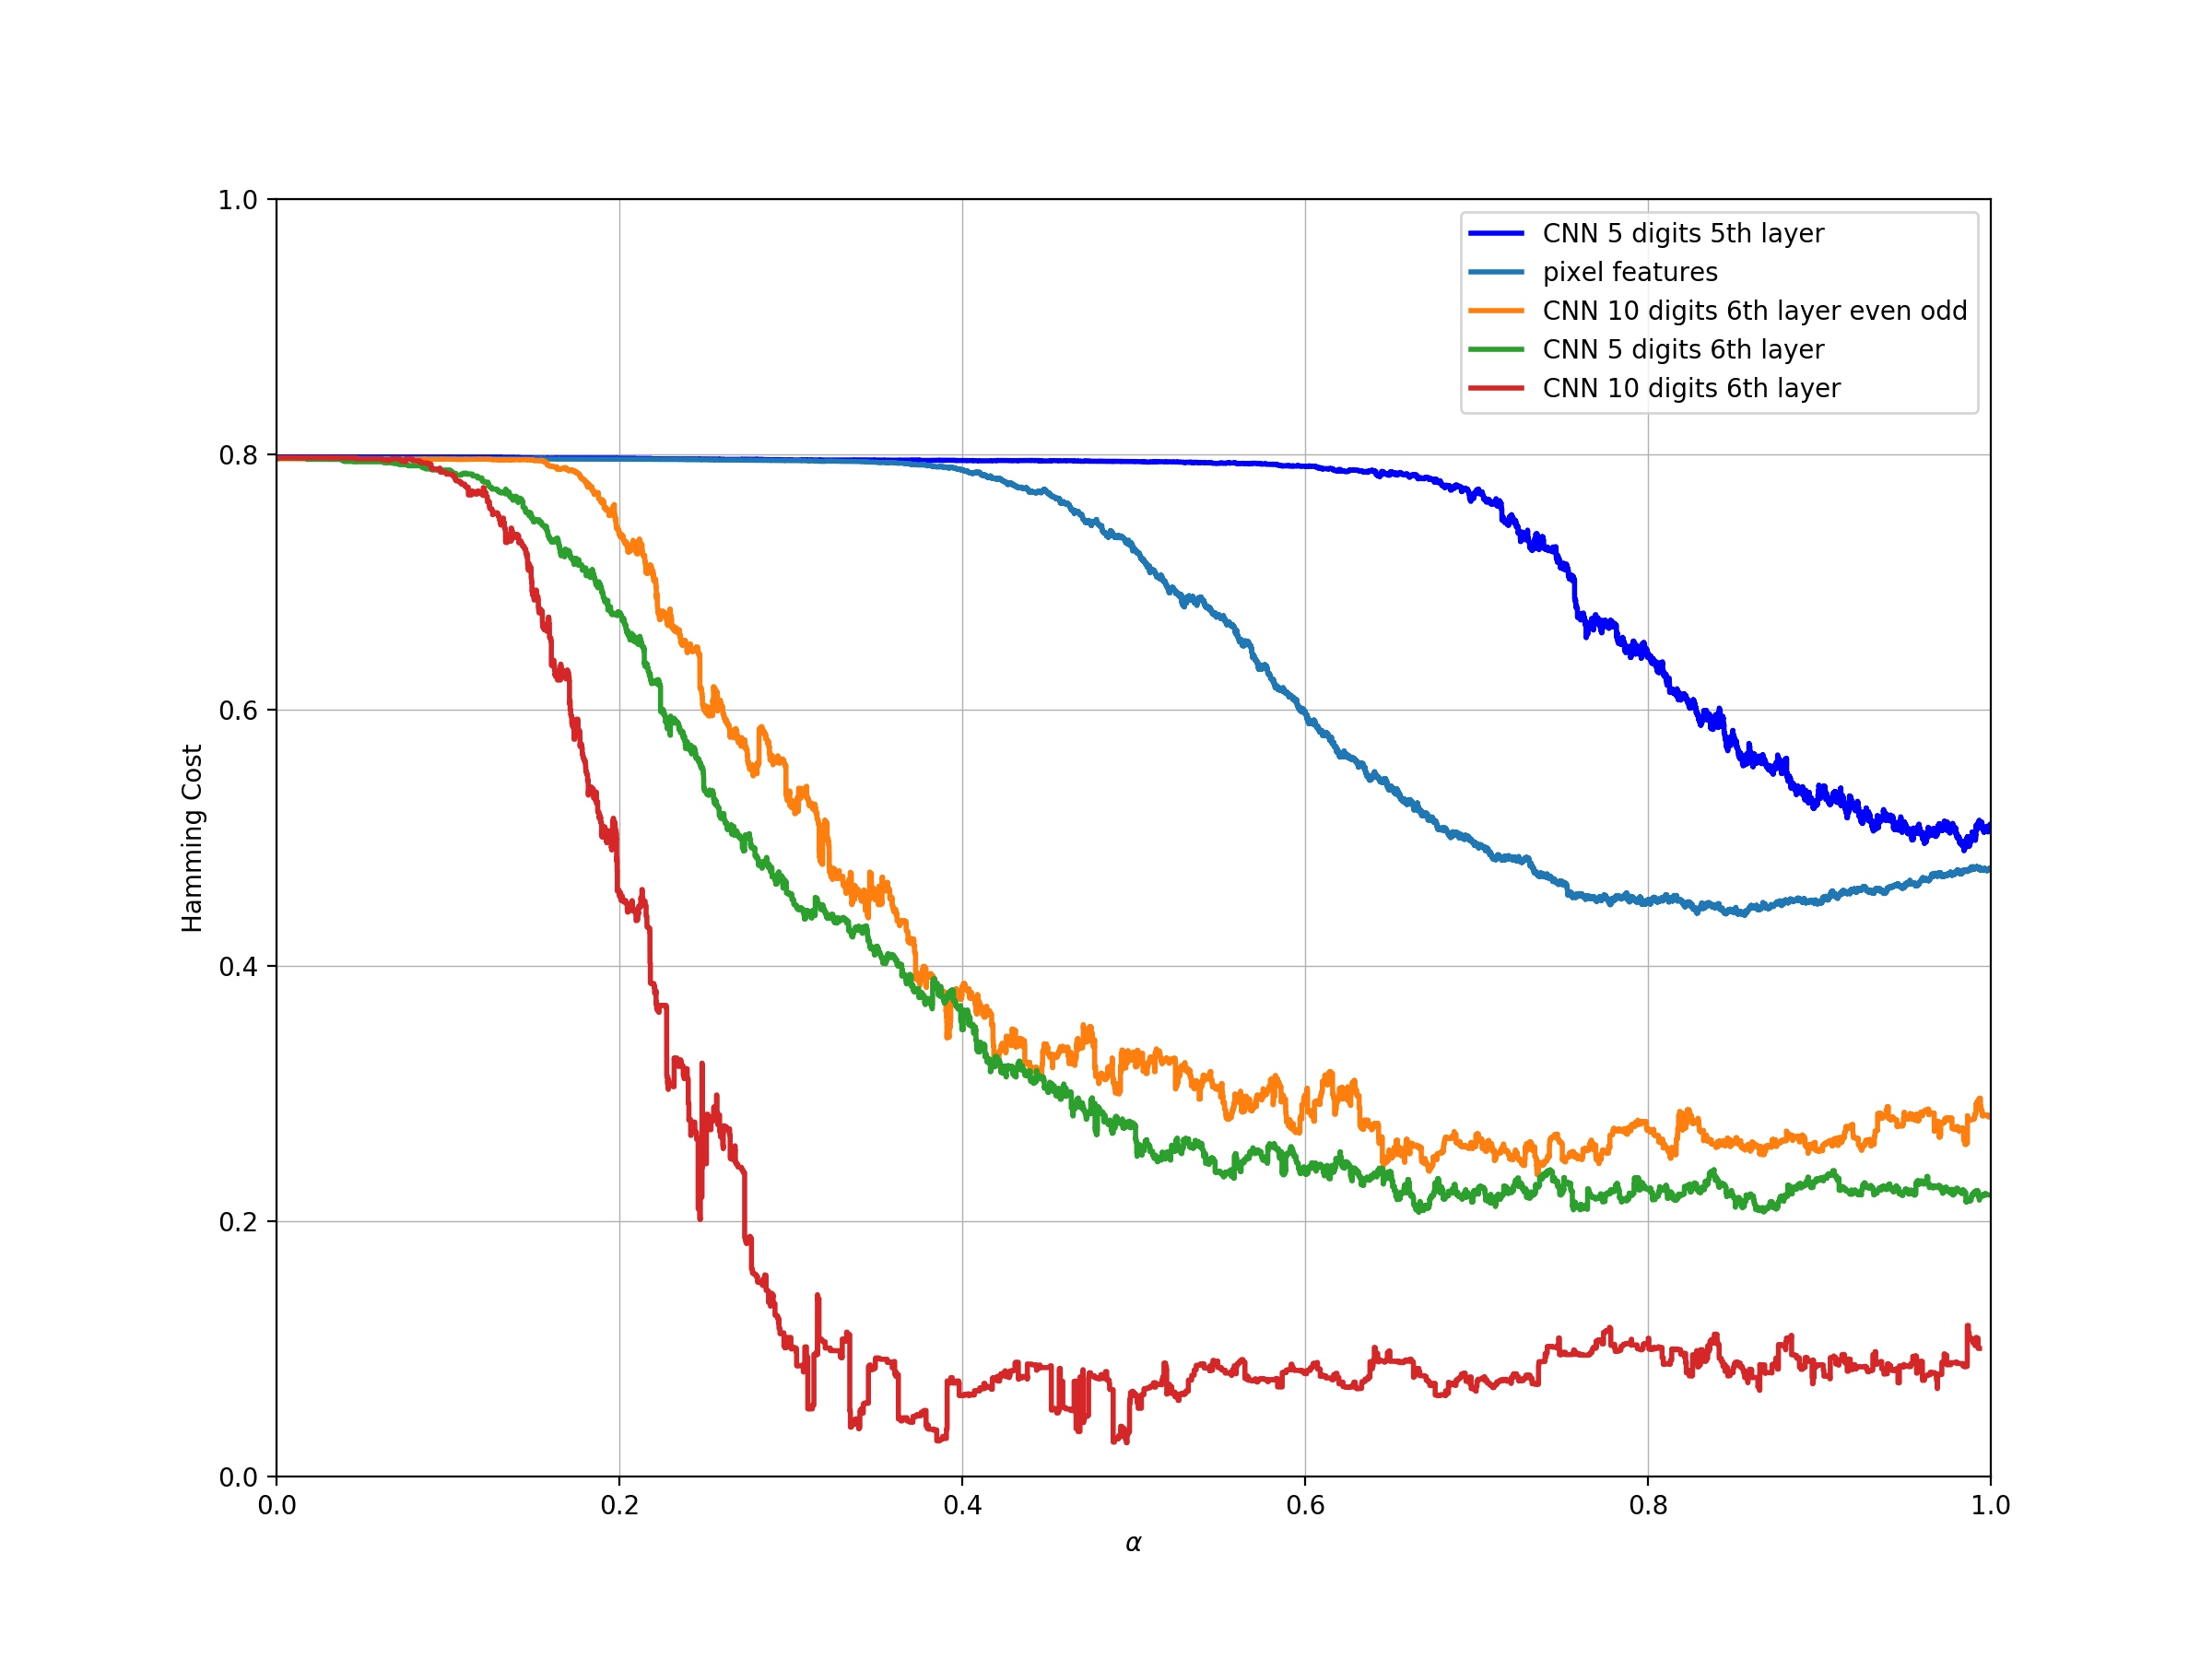
\includegraphics[width=\linewidth]{plots/mnist_overview}}
\end{minipage}\quad
\begin{minipage}{.45\textwidth}
  \centering
  \subcaptionbox{Evaluating 512 experiments with randomized digits and points shows similar results with smoother curves.}
  {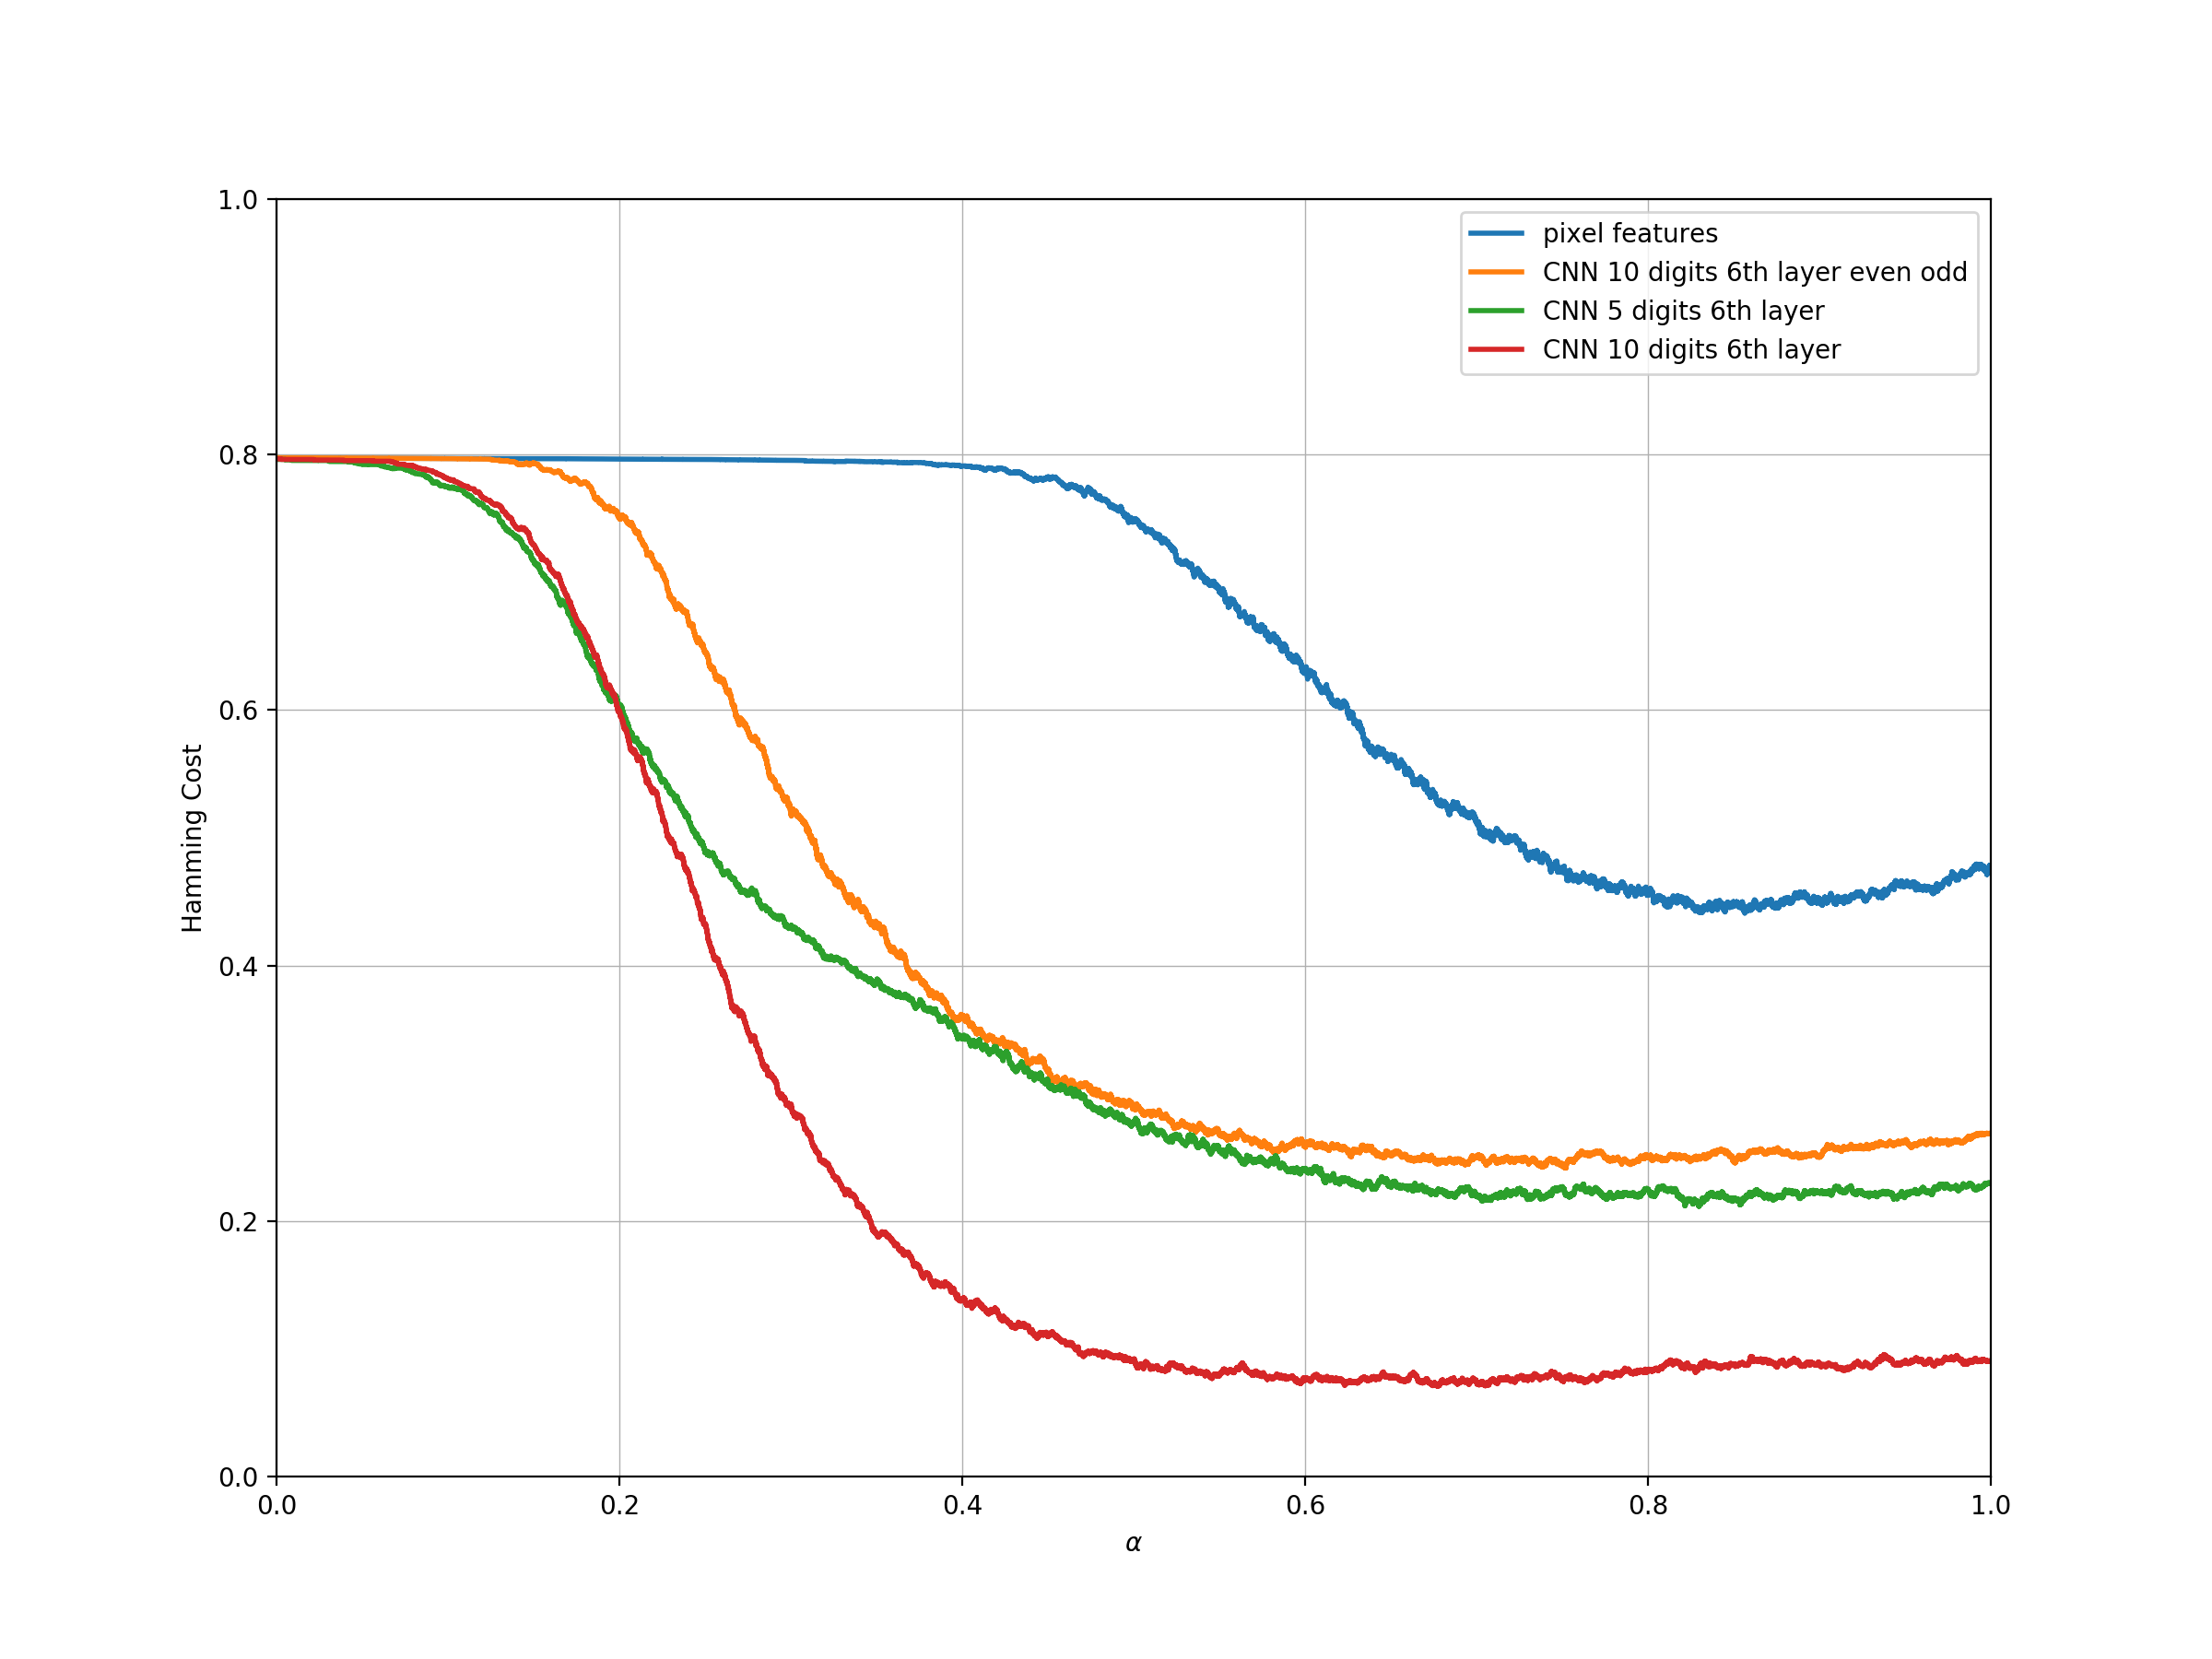
\includegraphics[width=\linewidth]{plots/mnist_overview_random}}
\end{minipage}
\caption{%
  %
  The previously discussed experiments led to different results. While using the features extracted from the fifth layer of the neural network did not lead to good results, features extracted from the sixth layer led to huge improvements. Over all settings, none of the optimal algorithms was one contained in the given $d_{sc}$ family. Depending on the feature representition we improved the clusterings by up to $7.4\%$ compared to complete linkage that outperformed single linkage in all settings.}
  %
\label{fig:mnist_overview}
\end{figure}

\paragraph{Omniglot Experiments.} The omniglot dataset contains 30 different alphabets that clustered independently. We cluster all alphabets independently and average over all clustering instances. To see the results for specific alphabets, please see appendix \ref{app:omniglot}. Here, we average the results over all alphabets for $\dsc$ and $\dac$. Figure \ref{fig:omniglotintra} shows ...

\begin{figure}[h]
\centering
\begin{minipage}{.45\textwidth}
  \centering
  \subcaptionbox{AC.}
  {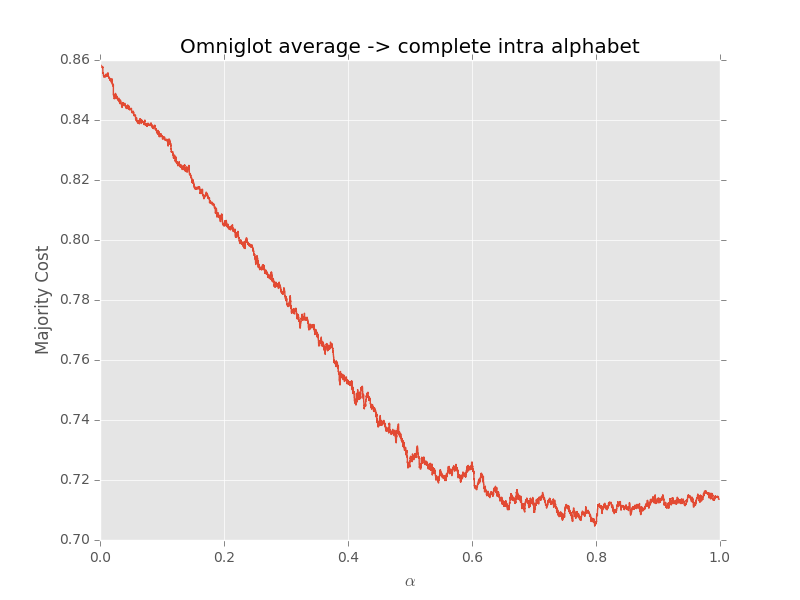
\includegraphics[width=\linewidth]{plots/omniglot-ac-average.png}}
\end{minipage}\quad
\begin{minipage}{.45\textwidth}
  \centering
  \subcaptionbox{SC.}
  {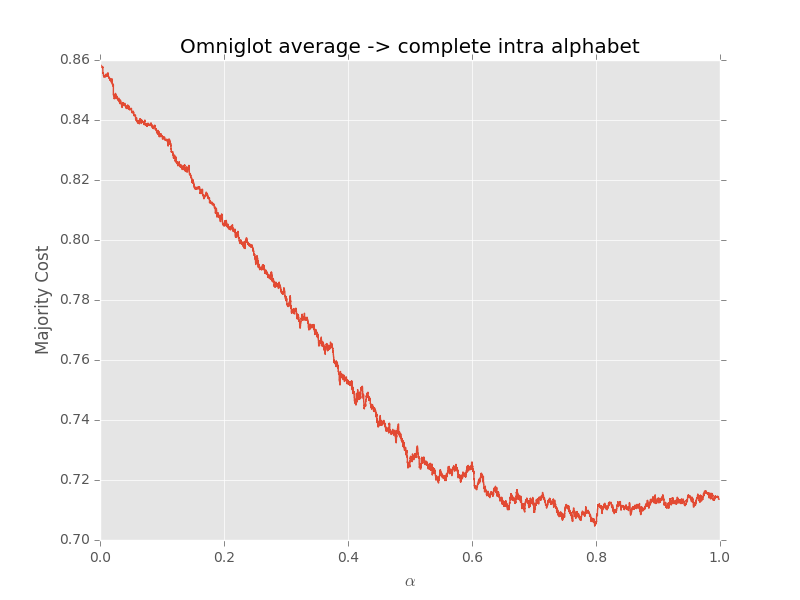
\includegraphics[width=\linewidth]{plots/omniglot-ac-average.png}}
\end{minipage}
\caption{%
  %
  Omniglot Intra.}
  %
\label{fig:omniglotintra}
\end{figure}

\todo[inline]{Update and evaluate plot.}

\paragraph{CNN Features.} In addition to clustering the raw pixels, we also used the previously discussed CNN architecture trained on all MNIST images to create a better feature representation. We again clustered all alphabets seperately, where we show the results for all alphabets in appendix \ref{app:omniglot}. Figure \ref{fig:omniglotintracnn} shows ...

\begin{figure}[h]
\centering
\begin{minipage}{.45\textwidth}
  \centering
  \subcaptionbox{AC.}
  {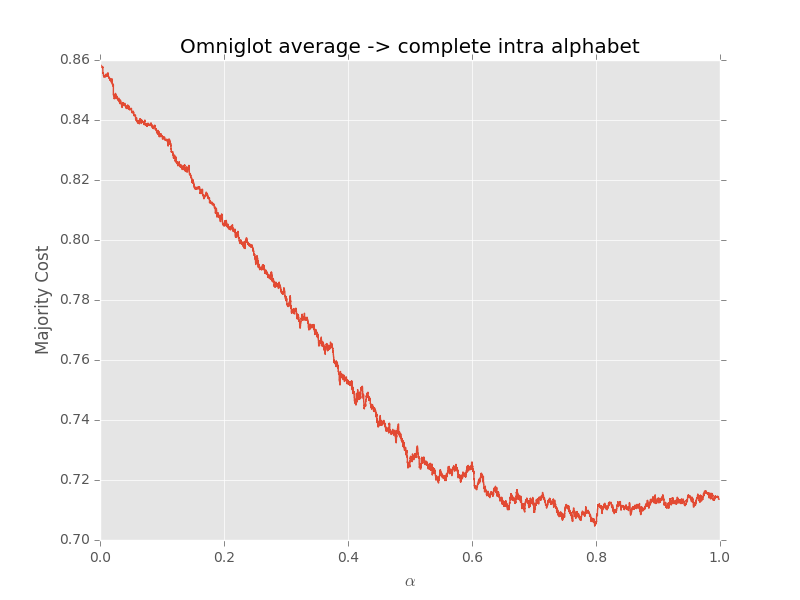
\includegraphics[width=\linewidth]{plots/omniglot-ac-average.png}}
\end{minipage}\quad
\begin{minipage}{.45\textwidth}
  \centering
  \subcaptionbox{SC.}
  {\includegraphics[width=\linewidth]{plots/omniglot-ac-average.png}}
\end{minipage}
\caption{%
  %
  Omniglot Intra CNN.}
  %
\label{fig:omniglotintracnn}
\end{figure}

\todo[inline]{Update and evaluate plot.}

\paragraph{Inter-Alphabet Experiments.} In addition, we tried to cluster characters taken from different alphabets. In our setting, we selected one character from each alphabet randomly and ran multiple repetitions of this setting where each run contains 30 classes, i.e. 600 points. One advantage of this setting is that each run has the same amount of target cluster that made it easier to average the results over all experiments. Figure \ref{fig:omniglotinter} shows that also for clustering characters of different alphabets the improvements are rather small. Averaged over 250 runs the improvement shown above was $1.0\%$.

\begin{figure}[h]
\centering
\begin{minipage}{.45\textwidth}
  \centering
  \includegraphics[width=\textwidth]{plots/omniglot-sc-average-inter}
\end{minipage}
\begin{minipage}{.45\textwidth}
  \centering
  \includegraphics[width=\textwidth]{plots/omniglot-ac-average-inter}
\end{minipage}
\caption{Clustering character of different alphabets only gives a small improvement for using the $\alpha$-linkage algorithm.}
\label{fig:omniglotinter}
\end{figure}

\paragraph{CIFAR Experiments.} In addition to these experiments, we will try to cluster as diverse as possible superclasses of the CIFAR100 dataset by manually picking the five superclasses fish, flowers, household furniture, people and vehicles 1. For each superclass we pick one subclass and evaluate the results for all $5 *$ $5 \choose 1$ $= 25$ different combinations of subclasses. In addition to the experiments with $k = 5$ clusters, we compare these results to the results for picking two different subclasses of each superclass ($5 *$ $5 \choose 2$ $= 50$ different experiments) resulting in $k = 10$ clusters and also for picking three different subclasses ($5 *$ $5 \choose 3$ $= 50$ different experiments) resulting in $k = 15$ clusters.\\

In comparison to picking as diverse as possible superclasses, we also evaluate the performance for as similar as possible subclasses. Similar subclasses are already given in the dataset through the subclasses within one superclass. We then evaluate the majority and the hamming cost for each superclass and again average the cost over all 20 superclasses to evaluate an optimal value for the parameter $\alpha$.

\section{Metric Learning}

\medskip\noindent\textbf{Omniglot.} First we present results on the omniglot
dataset \cite{Lake1332}.

\paragraph{Instance distributions.} We conduct experiments for two distributions
over clustering instances on the Omniglot dataset, both inspired by prior work
on few-shot meta-learning. Following \cite{NIPS2016_6385} and
\cite{pmlr-v70-finn17a}, our first instance distribution selects $k = 5$ random
characters (independently of their alphabet) and takes the 20 examples of those
5 characters resulting in a dataset with $n = 100$ examples. The target
clustering is given by the $5$ character labels. We refer to this instance
distribution as the MN/MAML distribution. Second, following
\cite{DBLP:journals/corr/abs-1903-03096}, our second instance distribution generates
clustering instances that have a variable number of target clusters and each
clustering task involves related characters. Specifically, to generate an
instance, we pick one alphabet from Omniglot uniformly at random, choose the
number of classes $k$ uniformly between $5$ and $10$, and then choose $k$
characters from that alphabet uniformly at random. As before, the clustering
instance consists of all $20k$ examples for the chosen characters, and the
target clustering is given by the $k$ character labels. We refer to this
instance distribution as the MD distribution.

\paragraph{Distance metrics.} We present results for mixing three different
distance metrics on the Omniglot data. This dataset provides two different
representations for each example: a $105 \times 105$ black and white image of
the character, and stroke data describing the path that the pen took when
writing that character (i.e., a time series of $(x,y)$ coordinates). We use a
hand-designed distance metric based on the stroke data, as well as features
derived from a convolutional neural network trained on MNIST.
%
\begin{itemize}
  %
  \item (Stroke distance) Given two pen stroke trajectories $s = (x_t,
  y_t)_{t=1}^T$ and $s' = (x'_t, y'_t)_{t=1}^T$, we define the distance between
  them by
  %
  \[
    d(s,s') = \frac{1}{T + T'} \left(
      \sum_{t=1}^T d\bigl((x_t, y_t), s'\bigr)
      +
      \sum_{t=1}^{T'} d\bigl((x'_t, y'_t), s\bigr)
    \right),
  \]
  %
  where $d\bigl((x_t, y_t), s'\bigr)$ denotes the Euclidean distance from the
  point $(x_t, y_t)$ to the closest point in $s'$. This is the average distance
  from any point from either trajectory to the nearest point on the other
  trajectory.
  %
  \item (CNN-C) Next we construct a distance metric using the image
  representation of each example. In particular, we train a convolutional neural
  network for classifying the 10 digits of MNIST. Then we use this network to
  obtain embeddings of each omniglot digit. Finally, to measure the distance
  between two examples, we use the cosine-distance between them (that is, the
  angle between the two feature embeddings).
  %
  \item (CNN-E) The final metric uses the same neural network embedding as
  above, except measures distances between two examples using the Euclidean
  distance.
  %
\end{itemize}

\paragraph{Results.} Figure \ref{fig:dl-omniglot} shows our empirical results for
learning the best combinations of the above metrics on both instance
distributions over the Omniglot dataset. For each pair of metrics and each
instance distribution, we plot the average Hamming error of the cluster tree
produced by the algorithm as a function of the mixing parameter $\beta$ averaged
over $N = 2000$ clustering instances sampled from the underlying distribution.
For both distributions, the best mixture of two metrics performs better than the
best fixed single metric. On the MN/MAML distribution, the best average
performance is obtained when mixing the Euclidean and cosine distances for the
MNIST CNN features with $\beta = 0.727$ achieving an average Hamming error of
$0.263$. In contrast, using the cosine distance on the MNIST CNN features is the
best single metric and has an average Hamming error of $0.289$, yielding an
improvement of $0.026$. For the MD instance distribution, the stroke distance
appears to be more useful. The best performance is achieved when mixing the
stroke distance and the cosine distance on the MNIST CNN features with $\beta =
0.514$ and achieves error $0.33$, while the best fixed metric has error $0.42$,
leading to an improvement of $0.09$.


\begin{figure}[H]
  \begin{subfigure}[b]{0.5\textwidth}
    \centering
    \includegraphics[width=0.9\textwidth]{plots/omniglot_MAML_results}
    \caption{MN/MAML Instance Distribution}
    \label{fig:dl-omniglot-maml}
  \end{subfigure}
  ~
  \begin{subfigure}[b]{0.5\textwidth}
    \centering
    \includegraphics[width=0.9\textwidth]{plots/omniglot_MD2_results}
    \caption{MD Instance Distribution}
    \label{fig:dl-omniglot-md}
  \end{subfigure}
  \caption{Learning the best distance metric for Omniglot.}
  \label{fig:dl-omniglot}
\end{figure}
